\documentclass[12pt, a4paper, oneside]{book}


\usepackage[italian]{babel}
\usepackage[T1]{fontenc}
\usepackage{amsthm}
\usepackage{amsmath}%
\usepackage{amsfonts}%
\usepackage{amssymb}%
\usepackage{graphicx}
\usepackage[utf8]{inputenc}
\usepackage{float}
\usepackage{url}
\usepackage{cite}


\usepackage{algorithm}
\usepackage{algpseudocode}

\usepackage{tkz-graph}  
\usepackage{tikz}
\usetikzlibrary{shapes.geometric, arrows}
\usetikzlibrary{arrows.meta}
\usetikzlibrary{decorations.pathreplacing}
\linespread{1.3}

\newtheorem{mydef}{Definition}
\newtheorem{theorem}{Theorem}
\newtheorem{observation}{Observation}
\newtheorem{corollary}{Corollary}
\newtheorem{proposition}{Preposition}
\newtheorem{lemma}{Lemma}
\newtheorem{example}{Example}


\usepackage[top=3.5cm, bottom=3.5cm, left=4cm, right=3.5cm]{geometry}


\renewcommand{\vec}{\bm}
\begin{document}

\tableofcontents
\pagenumbering{arabic}

\newpage
\thispagestyle{empty}
\listoffigures

\newpage
\thispagestyle{empty}
\section*{abstract}
Questa tesi si occupa di presentare le metodologie e GLI strumenti applicati nella realizzazione di una etichettatrice di flaconi ad alta velocità, progettata e sviluppata per l'area farmaceutica.
Verranno presentati i processi necessari allo sviluppo software, sia per quanto riguarda la parte PLC sia la parte SCADA/HMI, nonché quella relativa allo sviluppo del sistema di visione e controllo.
Si analizzeranno i vari dispositivi che compongono il macchinario, il loro funzionamento ed in particolar modo i protocolli di comunicazione che ci permettono di dialogare con essi. 
Verrà affrontata inoltre la tematica dell'Industria 4.0 spiegando come poter sviluppare un sistema software che rispetti i criteri del nuovo standard nell'automazione Industriale.
 

\newpage
\thispagestyle{empty}
\section*{Introduzione al progetto}
Questa tesi si propone di presentare gli step necessari per lo sviluppo di una Etichettatrice ad alta velocità. Come noto, queste rappresentano componenti fondamentali nelle linee di produzione e richiedono qualità ed affidabilità. 
\\La tesi è stata sviluppata durante un periodo di tirocinio di cinque mesi presso la SPH, azienda specializzata nella realizzazione ex novo di macchine automatizzate per le industrie, in particolare quella farmaceutica. Durante lo sviluppo della tesi sono stato perciò affiancato da svariate figure professionali come ingegneri meccanici ed informatici, elettricisti, meccanici nonchè clienti di svariate aziende italiane ed estere. Il mio ruolo, ovvero quello di ingegnere informatico,  consiste nella progettazione e sviluppo di tutti i sistemi software necessari all'automatizzazione della macchina. 
\\Lavorare in SPH è tuttora un'esperienza altamente formativa e stimolante, perché non solo mi permette di approfondire le mie conoscenze nell'ambito della programmazione, ma propone ogni giorno nuove sfide e problematiche multidisciplinari da risolvere in team. Il contatto con il cliente, la stima del capo e il confronto con validi colleghi sono infine piacevoli aspetti del lavoro in SPH, un'azienda all'avanguardia in crescita e affermazione nel mercato dell'automazione industriale.   
\\Nel primo capitolo verrà presentata la struttura della Etichettatrice LabelTech, presentandone una descrizione sulla struttura meccanica, sui dispositivi elettrici ed elettronici che la compongono ed infine illustrandone il funzionamento.
\\Nel secondo capitolo viene descritto il processo di sviluppo software che è stato seguito nella realizzazione del progetto: in particolare verranno illustrate le tecniche ed i passi da seguire, insieme con le best practice per un corretto design del software. Infine verranno presentati le Camme Digitali e Shift-Register necessari nei Sistemi di Contollo.
\\Nel Capitolo 3 verranno presentati i protocolli di comunicazione di norma utilizzati nell'ambito dell'automazione industriale, con particolare attenzione sui BUS Profinet, sulla Pila Protocollare TCP/IP e sull'Open Platform Communication, il nuovo standard utilizzato in ambito industriale.
\\Nel Capitolo 4 si parlerà dei Sistemi di Visione, in particolare dei sistemi Datalogic e del loro sviluppo: il sistema di visione è infatti un controllore necessario ed efficace nella verifica di tutti i pezzi e di tutta la produzione continua, assicurando che nessuna parte di questa sia non conforme alle specifiche prestabilite.
\\Nel Capitolo 5 descriveremo le Tipologie di Human Machine Interface, ovvero lo strato che separa un essere umano che sta usando una macchina dalla macchina stessa. Si parlerà nel dettaglio di come progettare un'interfaccia HMI/SCADA, come permettere la comunicazione tra questa ed il PLC, e le normative in vigore nell'ambito del settore Farmaceutico e più in generale dell'Industria 4.0.
\\Infine nel Capitolo 6 verranno estratte le conclusioni sul progetto e sull'esperienza maturata durante il periodo di tirocinio in SPH, accennando brevemente gli sviluppi futuri del lavoro.

\chapter{Etichettatrice LabelTech}
In questo capitolo spiegheremo il funzionamento dell'Etichettatrice. A tal scopo è necessario presentare una breve descrizione sulla struttura meccanica, per poi passare ad una dettagliata analisi dei dispositivi Elettrici ed Elettronici che la compongono.
\section{Struttura Meccanica}
In questa sezione descriviamo la struttura meccanica analizzando i vari elementi che la compongono.
La meccanica base dell'Etichettarice è relativamente semplice. Come si può ben vedere nella figura \ref{mec1} essa è composta da tre stelle trasportatrici: la prima è quella di ingresso (1) che si occupa di agganciare i flaconi dal nastro di ingresso. La seconda, ovvero quella centrale (2) più grande, è la stella principale che trasporta i flaconi sull'unità di etichettaggio. L'ultima è la stella di uscita (3) che si occupa di trasportare i flaconi verso l'uscita e di scartare eventuali flaconi che non hanno superato i controlli di qualità. Quest'ultima, per gestire lo scarto, ha in ogni incavo una ventosa che serve a catturare il flacone scartato per evitare che venga rilasciato sul nastro di uscita. Il meccanismo di scarto verrà descritto in dettaglio nel capitolo 2.
\\Un altro elemento della struttura meccanica base è il massaggiatore (4) che si occupa di assicurare l'adesione dell'etichetta nella fase appena successiva all'applicazione sul flacone. Esso è costituito da una cinghia gommata messa in moto da un sistema di rulli dentati, alimentati da un motore brushless.

\begin{figure}[H]
	\centering
	\includegraphics[width=12cm]{Immagini/MEC1}
	\label{mec1}
	\caption{ Vista dall'alto della struttura della macchina}
\end{figure}

Nella figura \ref{mec2} si possono osservare chiaramente i tre ingranaggi delle tre stelle, il motore con il riduttore collegato alla stella principale, la stella di uscita ed il sistema pneumatico necessari a gestire lo scarto dei flaconi.

\begin{figure}[H]
	\centering
	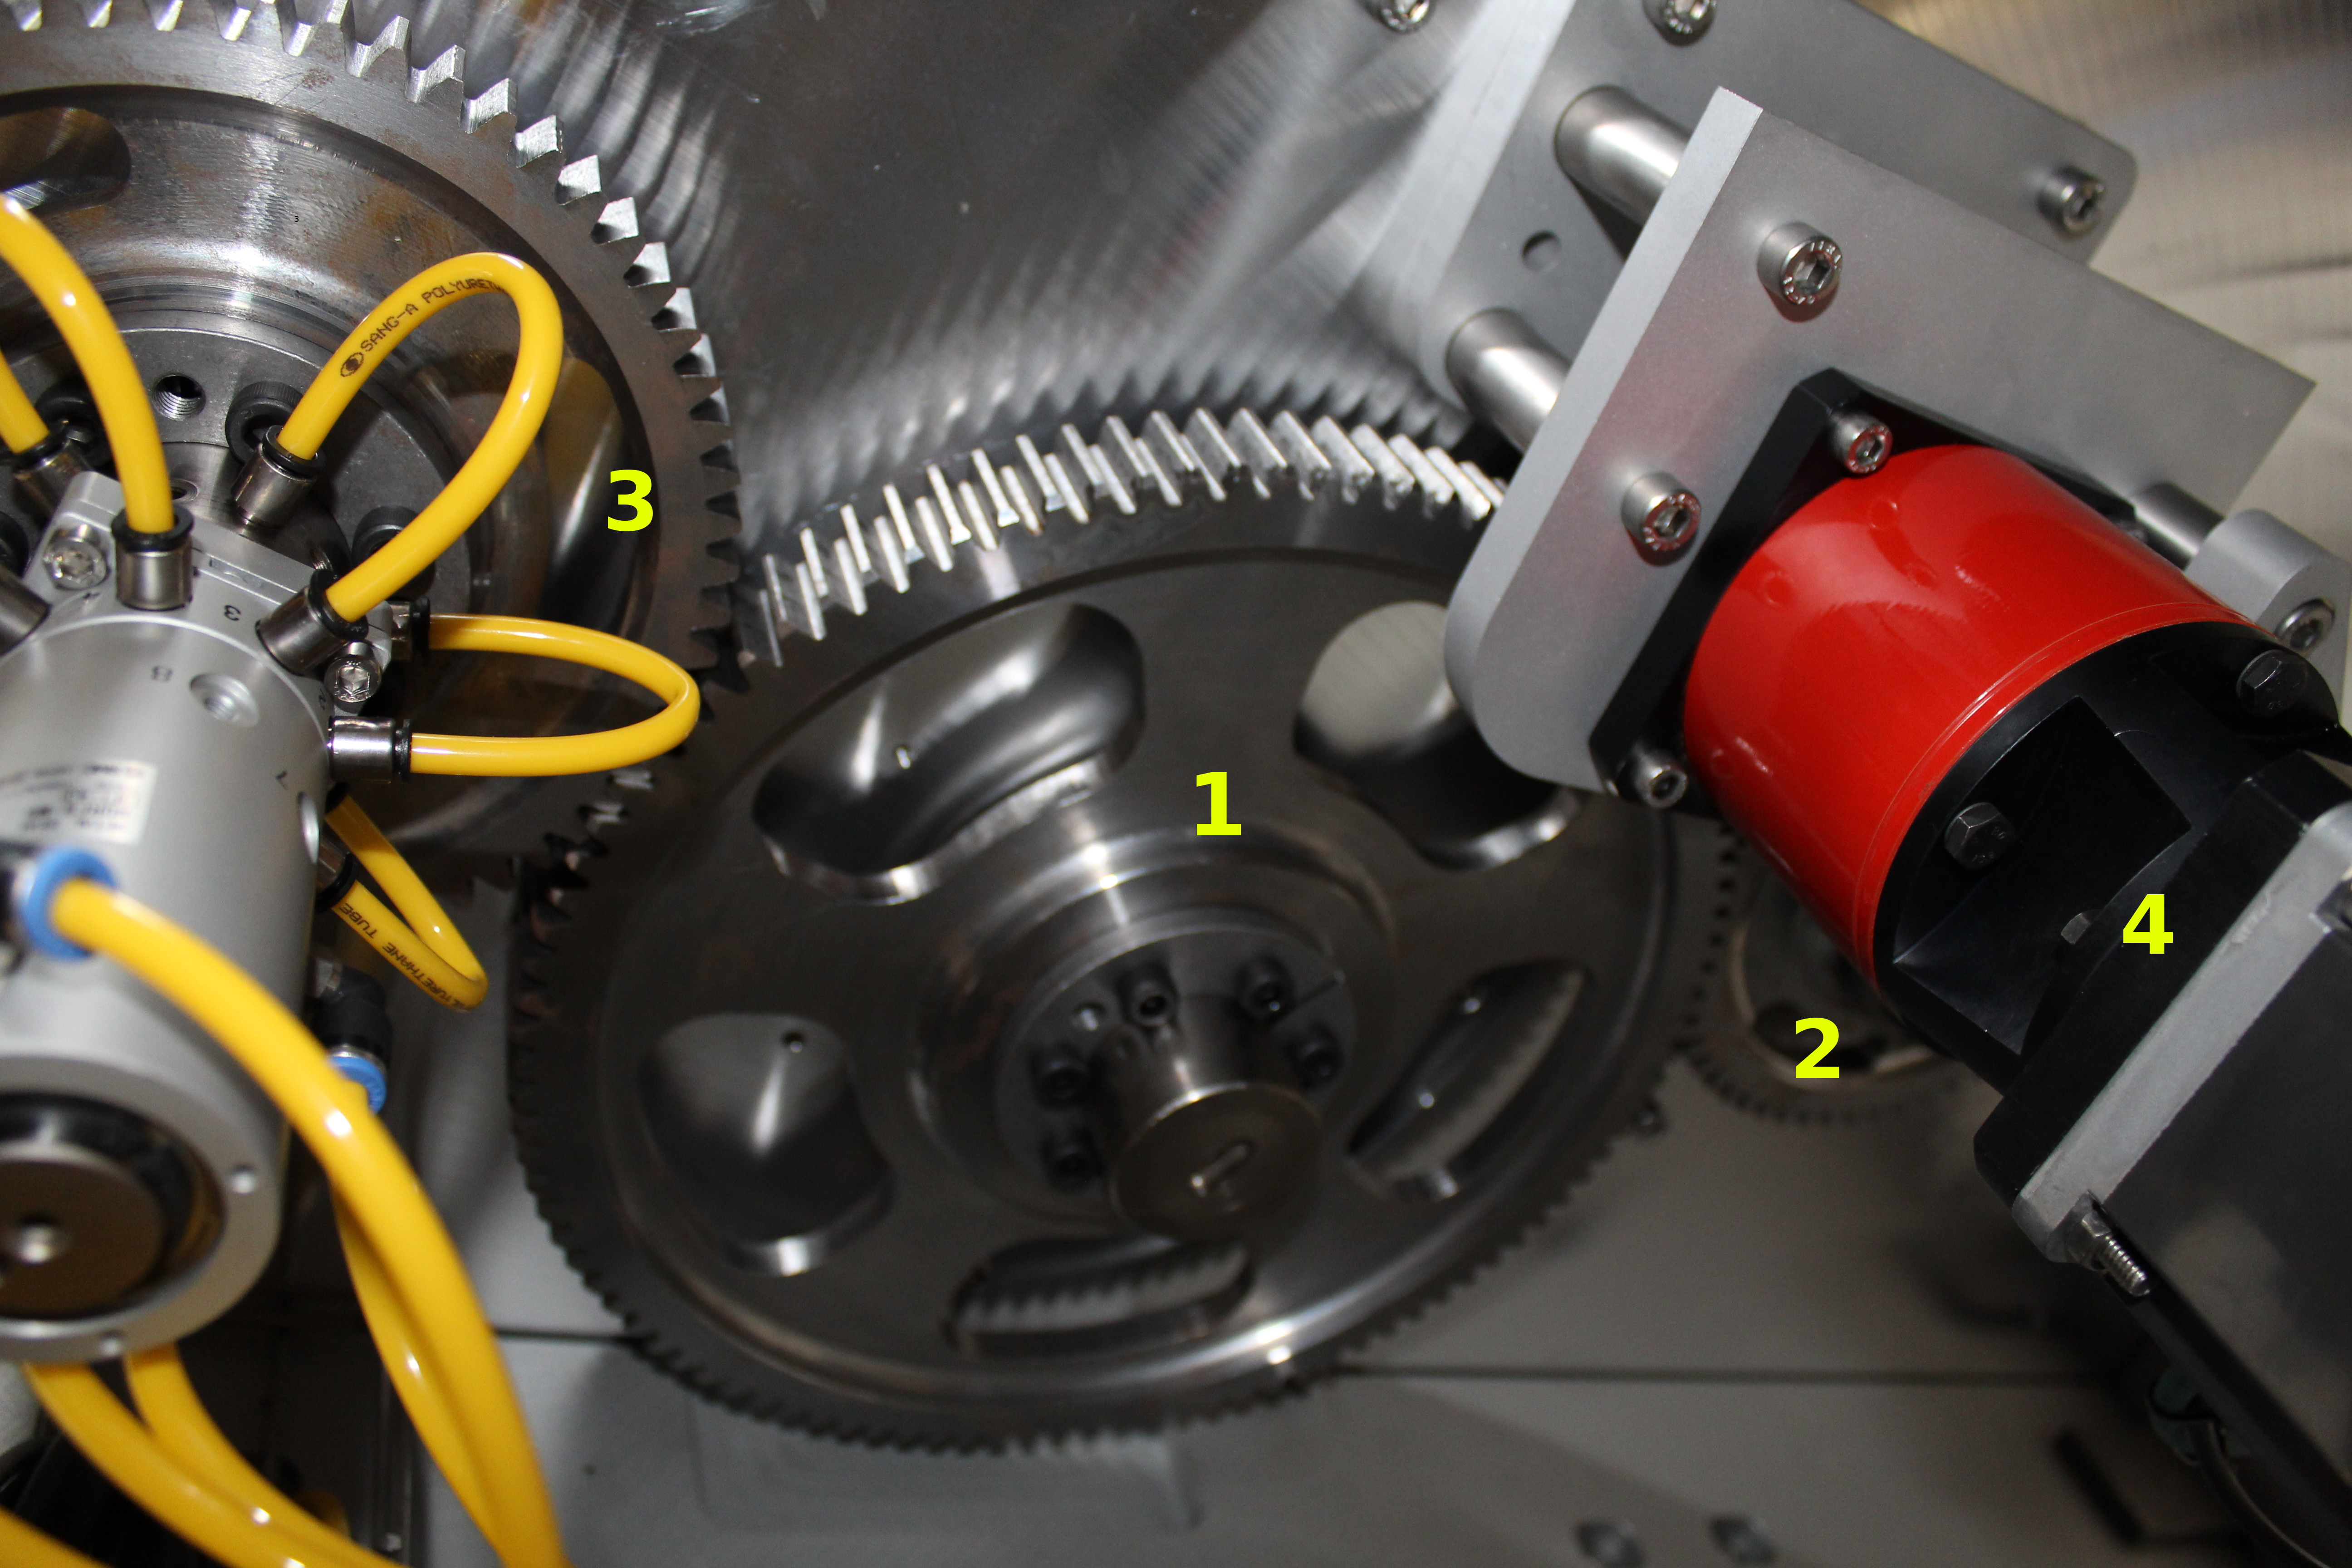
\includegraphics[width=12cm]{Immagini/MEC2}
	\label{mec2}
	\caption{ Vista sotto scocca della struttura della macchina}
\end{figure}


\section{Dispositivi Elettrici ed Elettronici}
I dispostivi elettrici ed elettronici che compongono l'etichettatrice sono molteplici. Essi rappresentano l'anima della macchina stessa in quanto permettono a tutto il processo di prendere vita.
Di seguito sono elencati i vari dispositivi dell'etichettatrice.

\begin{itemize}
	
	\item \textit{HERMA 400 Labeling Machine}	
	L'elemento più importante di tutta la macchina è proprio il gruppo di etichettatura che, sebbene risulti essere un ibrido tra meccanica ed elettronica, è presentato in questa sezione perchè è completamente gestito da una scheda interna, presentando vari sensori e dispositivi necessari al proprio funzionamento.
	

	
	\begin{figure}[H]
		\centering
		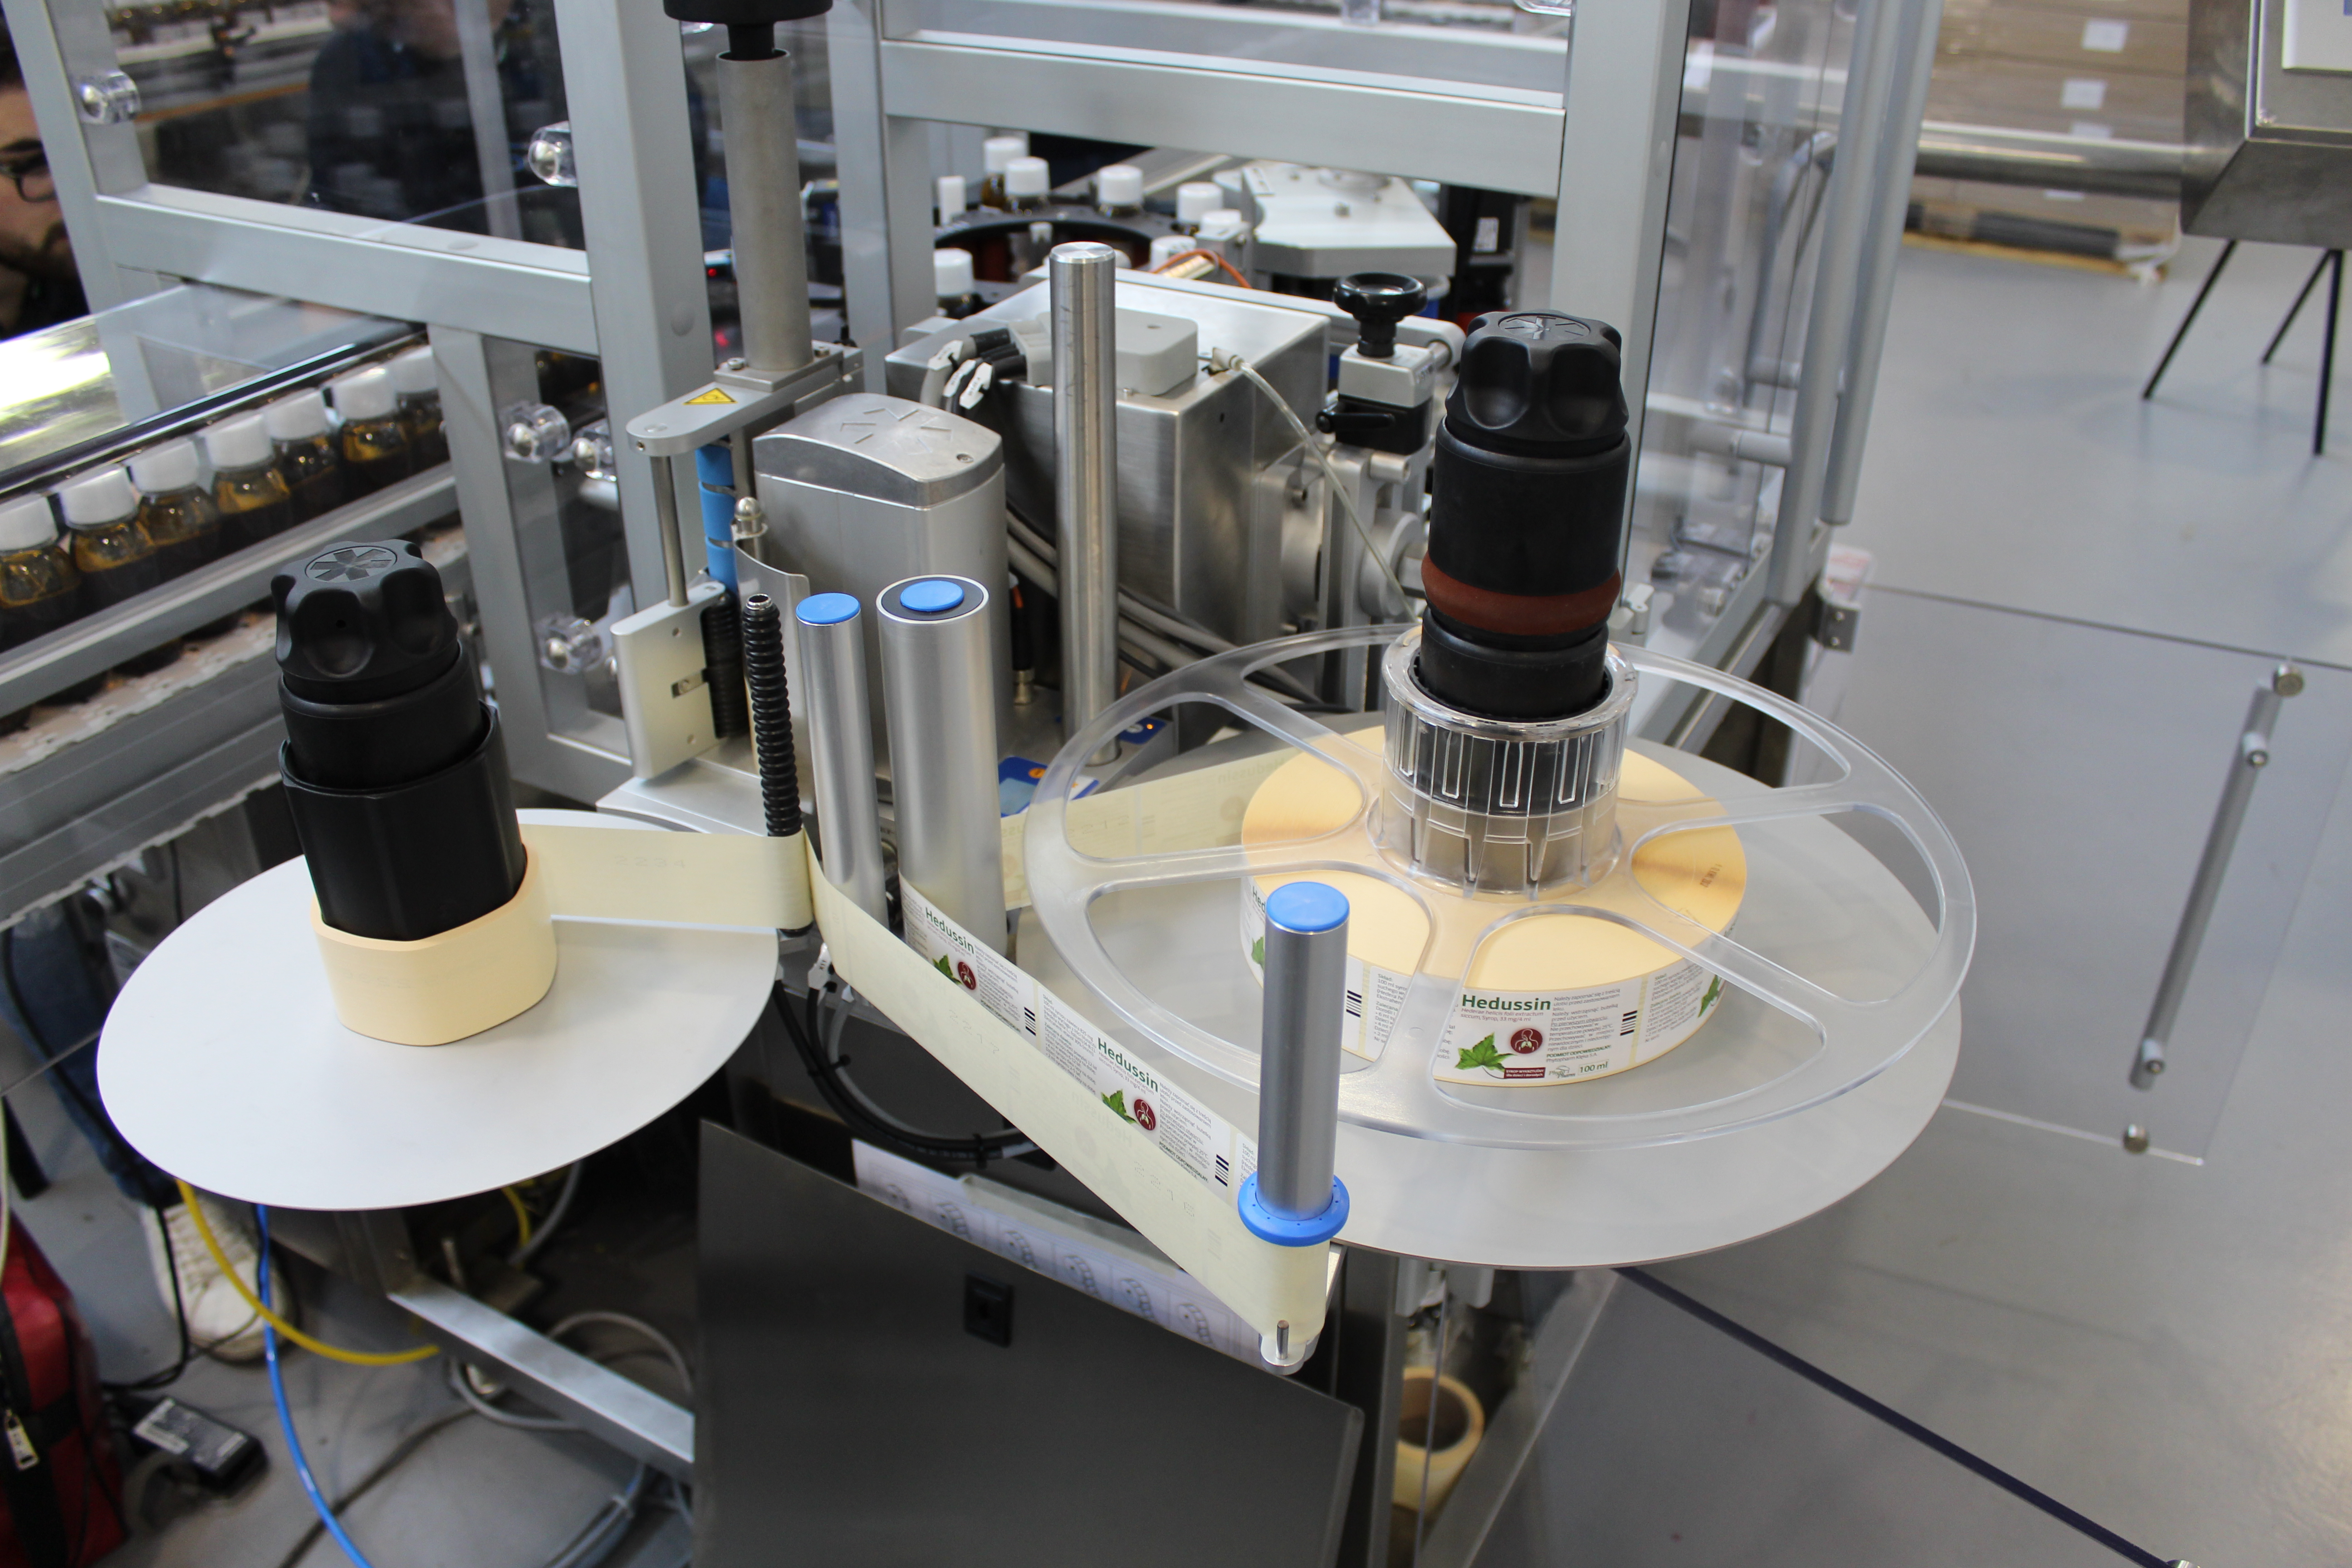
\includegraphics[width=12cm]{Immagini/ELE1}
		\label{ele1}
		\caption{HERMA 400}
	\end{figure}
	
	
	Il gruppo di etichettatura della Herma è un dispositivo molto efficiente e complesso. Ha una velocità di etichettatura che può andare ben oltre i 400 pz/min ed è facilmente integrabile in qualsiasi sistema, poiché richiede pochissimi accorgimenti esterni. Non è inoltre necessario riconfigurare i vari formati di etichetta poiché essa dispone di un sensore di autoapprendimento che determina la lunghezza dell'etichetta \ref{ele2}.
	
		\begin{figure}[H]
		\centering
		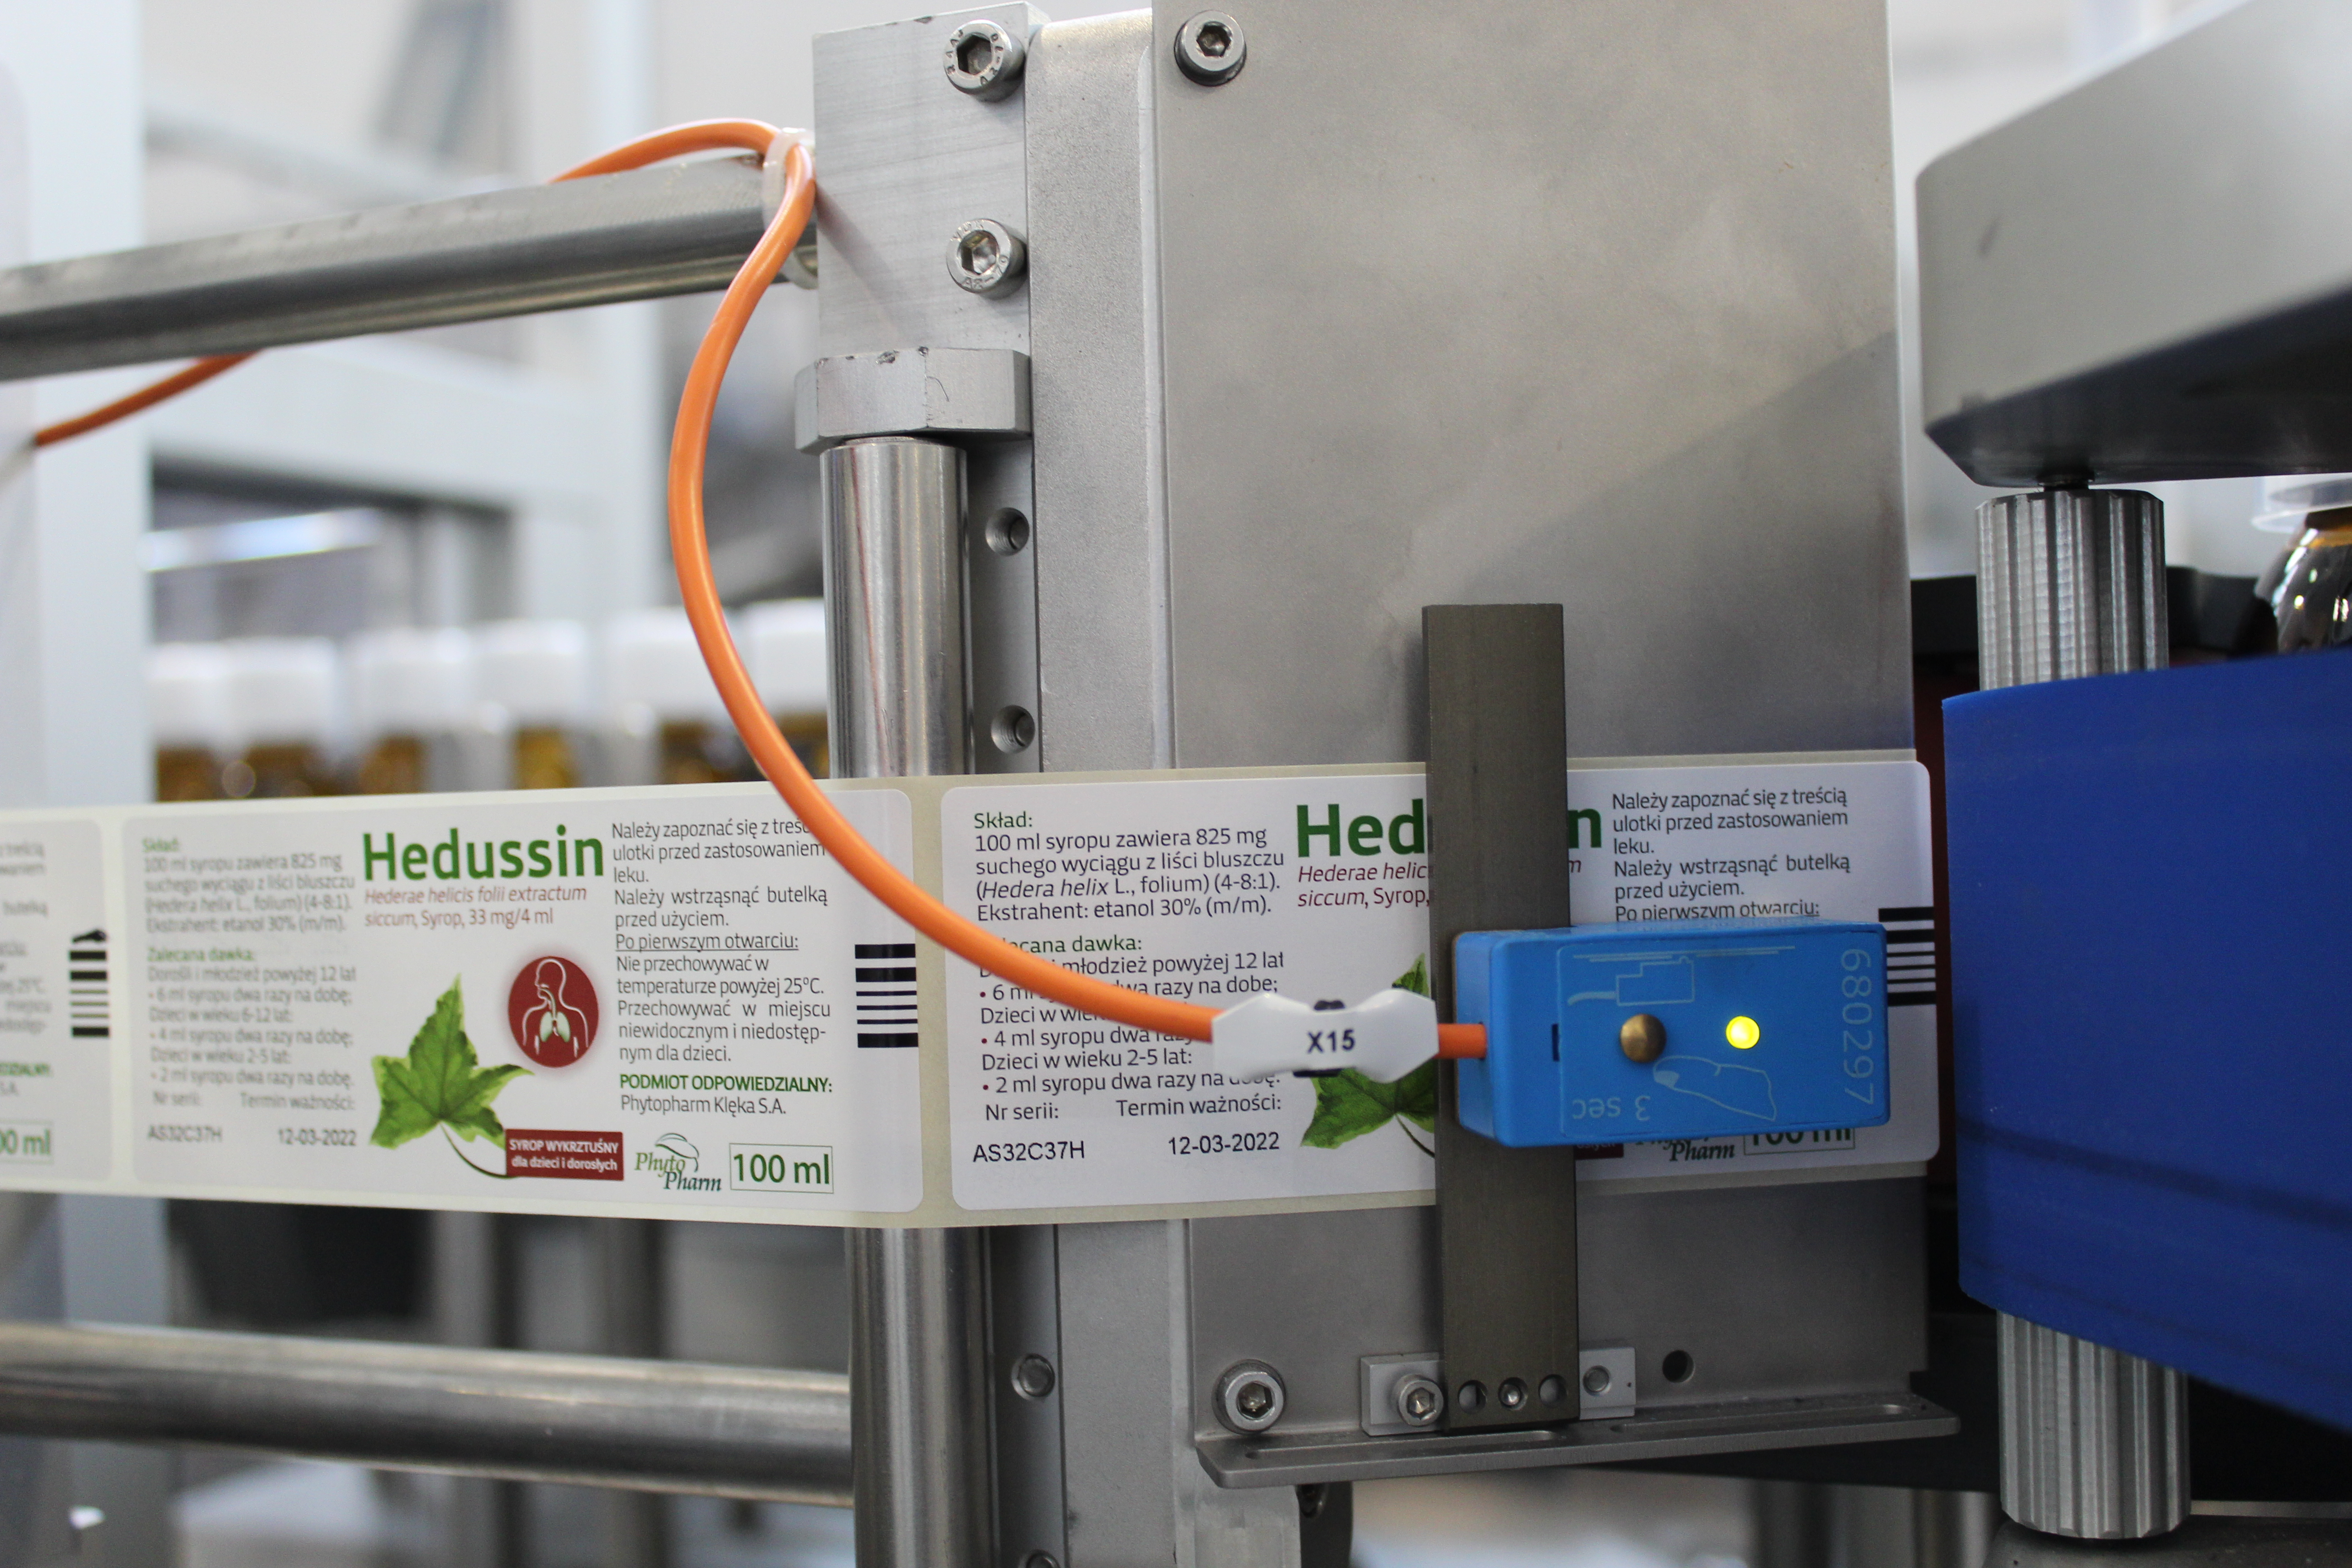
\includegraphics[width=12cm]{Immagini/ELE2}
		\label{ele2}
		\caption{HERMA 400 Sensore Autoapprendimento}
	\end{figure}
	
	 Per ottimizzare l'etichettatura la Herma mette a disposizione un particolare encoder da collegare al massaggiatore della macchina. Grazie ad esso essa regola automaticamente la velocità con la quale espellere l'etichetta. L'unico comando necessario all'etichettatrice per poter funzionare è un trigger digitale che comanda l'espulsione di una etichetta. Naturalmente è difficile determinare se e quando dare il comando. Ma questo è un problema che analizzeremo nei capitoli relativi alla programmazione del software plc ed al controllo mediante sistema di visione.  
	
	\item \textit{Mitsubishi HG-Series Motors}
	Sono i motori utilizzati sia dal motore principale che dal massaggiatore. Sono dei motori brushless ad elevatissime prestazioni ed estremamente compatti. Posso essere utilizzati standalone oppure, come nel nostro caso, mediante degli specifici azionamenti che ne consentono un pieno controllo. 
	
	\begin{figure}[H]
		\centering
		\includegraphics[width=8cm]{Immagini/ELE3}
		\label{ele3}
		\caption{Motore Brushless Mitsibishi HG-Series}
	\end{figure}
	
	\item \textit{Mitsubishi MR-J4-TM Servo}
	Si riferisce agli azionamenti utilizzati per la gestione e controllo dei servo motori Mitsubishi. Esistono in vari modelli in base alla comunicazione necessaria. Nel nostro caso abbiamo optato per la versione con il Profinet poiché lavoriamo con un PLC Siemens. Questo consente di inviare comandi dal PLC all'azionamento e pertanto comandare il motore. Le specifiche metodologie di comunicazione verranno descritte nel capitolo 3.
	
		\begin{figure}[H]
		\centering
		\includegraphics[width=5cm]{Immagini/ELE4}
		\label{ele4}
		\caption{Azionamento Profinet Mitsubishi MR-J4-TM}
	\end{figure}
	
	\item \textit{Mitsubishi FR-D700SC}
	È un particolare inverter Mitsubishi che permette di comandare la velocità di un qualsiasi motore agendo sulla frequenza. Essa permette il controllo della velocità mediante un segnale analogico in tensione che va dai 0 ai 10V. Questo segnale può essere inviato da qualunque sorgente, nel nostro caso il PLC (in particolare dal modulo di uscita Analogica). Essa dispone inoltre di un comando digitale a contatto pulito che ne consente lo start and stop. Questo Inverter è stato utilizzato per poter gestire la velocità del nastro trasportatore pricipale di ingresso e uscita.
	
	\begin{figure}[H]
		\centering
		\includegraphics[width=6cm]{Immagini/ELE6}
		\label{ele6}
		\caption{Inverter di Frequenza Mitsubishi FR-D700SC}
	\end{figure}
	
	\item \textit{Datalogic P-Series}
	Sono le telecamere di Visione che si occupano di tutto il controllo qualità della macchina. Esse sono delle telecamere estremamente performanti con risoluzione di 1.3MP a Colori, compatibile con vari sistemi di comunicazione tra cui TCP-EtherCat-Profinet. Sono programmabili con oltre 30 tool di ispezione mediante il software proprietario Impact. Nell'etichettatrice ne sono stati applicati due: una prima telecamera per il controllo validità delle stampe dell'etichette (prima che esse vengano applicate sul flacone) e una seconda per verificare l'eventuale presenza ed allineamento dell'etichetta (successivamente all'applicazione).
	
	\begin{figure}[H]
		\centering
		\includegraphics[width=8cm]{Immagini/ELE5}
		\label{ele5}
		\caption{Inverter di Frequenza Mitsubishi FR-D700SC}
	\end{figure}
	
	\item \textit{VideoJet DataFlex 6530}
	È una stampante termica per utilizzo in applicazioni industrial ad alta velocità. Essa riesce a stampare con una freqenza oltre le 300 stampe per minuto. Dispone di un server web integrato per la configurazione oppure di un pannello LCD esterno. La comunicazione avviene tramite uno standard I/O e tramite TCP. Questa stampante viene utilizzata per stampare sull'etichetta i dati relativi al lotto attivo (quali nome e scadenza) ed anche a stampare il pharmacode (un particolare datamatrix utilizzato nel campo pharmaceutico)
	
		\begin{figure}[H]
	\centering
	\includegraphics[width=8cm]{Immagini/ELE8}
	\label{ele8}
	\caption{Stampante Termica VideoJet DataFlex 6530}
	\end{figure}
	
	\item \textit{Sick Encoder AFM60 PROFINET}
	Si tratta di un encoder assoluto a 30 bit di alta risoluzione.
	Possiede un'interfaccia profinet il che lo rende estremamente compatibile e semplice da gestire con il PLC siemens. Ha un tempo di aggiornamento dati inferiore a 5 ms e tramite profinet è capace di comunicare allarmi, avvertenze e funzioni di diagnosi per velocità, posizione, temperatura, durata del funzionamento ecc. Questo encoder è stato montato sul meccanismo della stella in ingresso in modo da tener traccia della posizione della macchina in tempo reale e pertanto gestire le varie camme della macchina.

		\begin{figure}[H]
	\centering
	\includegraphics[width=8cm]{Immagini/ELE7}
	\label{ele7}
	\caption{Encoder Profinet Sick AFM60}
	\end{figure}

	\item \textit{Siemens Simatic ET200S e Moduli I/0}	
	PLC controller con CPU-1510SP-SIMATIC-DP(1) è una unità centrale con 100kb di memoria lavoro e 750KB per i dati. Dispone di un'interfaccia Profinet ed ha una performance di bit di 72NS. Necessita di una memory card Simatic Siemens per il programma.
	La sua programmazione avviene tramite la suite Siemens WinCC conosciuta ora come tiaPortal. 
	Si ricorda che questa unità centrale non dispone di ingressi ed uscite pertanto necessita di moduli aggiuntivi. Nello specifico caso sono stati aggiunti ben 6 moduli di cui:
	\begin{itemize}
		\item \textit{3 Moduli di 16 Ingressi Digitali(2)}
		\item \textit{2 Moduli di 16 Uscite Digitali(3)}
		\item \textit{1 Modulo di 4 Uscite Analogiche(4)}
	\end{itemize}

	\begin{figure}[H]
	\centering
	\includegraphics[width=8cm]{Immagini/ELE11}
	\label{ele11}
	\caption{Siemens Simatic ET200S}
	\end{figure}

	\item \textit{ASEM HMI Panel HT2150}
	Panel PC da 12 pollici basata con processore Celeron J1900 quad core 2GHz a 64 bit.	La motherboard include due porte Ethernet 10/100/1000Mbps con supporto alle funzionalità 'Jumbo Frame' e 'Wake on Lan', una porta USB 2.0, una porta USB 3.0 ed uno slot per CFast SATA II ad accesso esterno posteriore, un connettore mSATA per l'installazione di una SSD SATA II, RAM fino a 8 GB con un modulo SODIMM DDR3 e un connettore interno per l'installazione di interfacce seriali e USB aggiuntive.
	Sistema Operativo Microsoft Windows Embedded 7.0
	
	\begin{figure}[H]
		\centering
		\includegraphics[width=8cm]{Immagini/ELE9}
		\label{ele9}
		\caption{ASEM HMI Panel HT2150}
	\end{figure}
	
	\end{itemize}

	\begin{figure}[H]
	\centering
	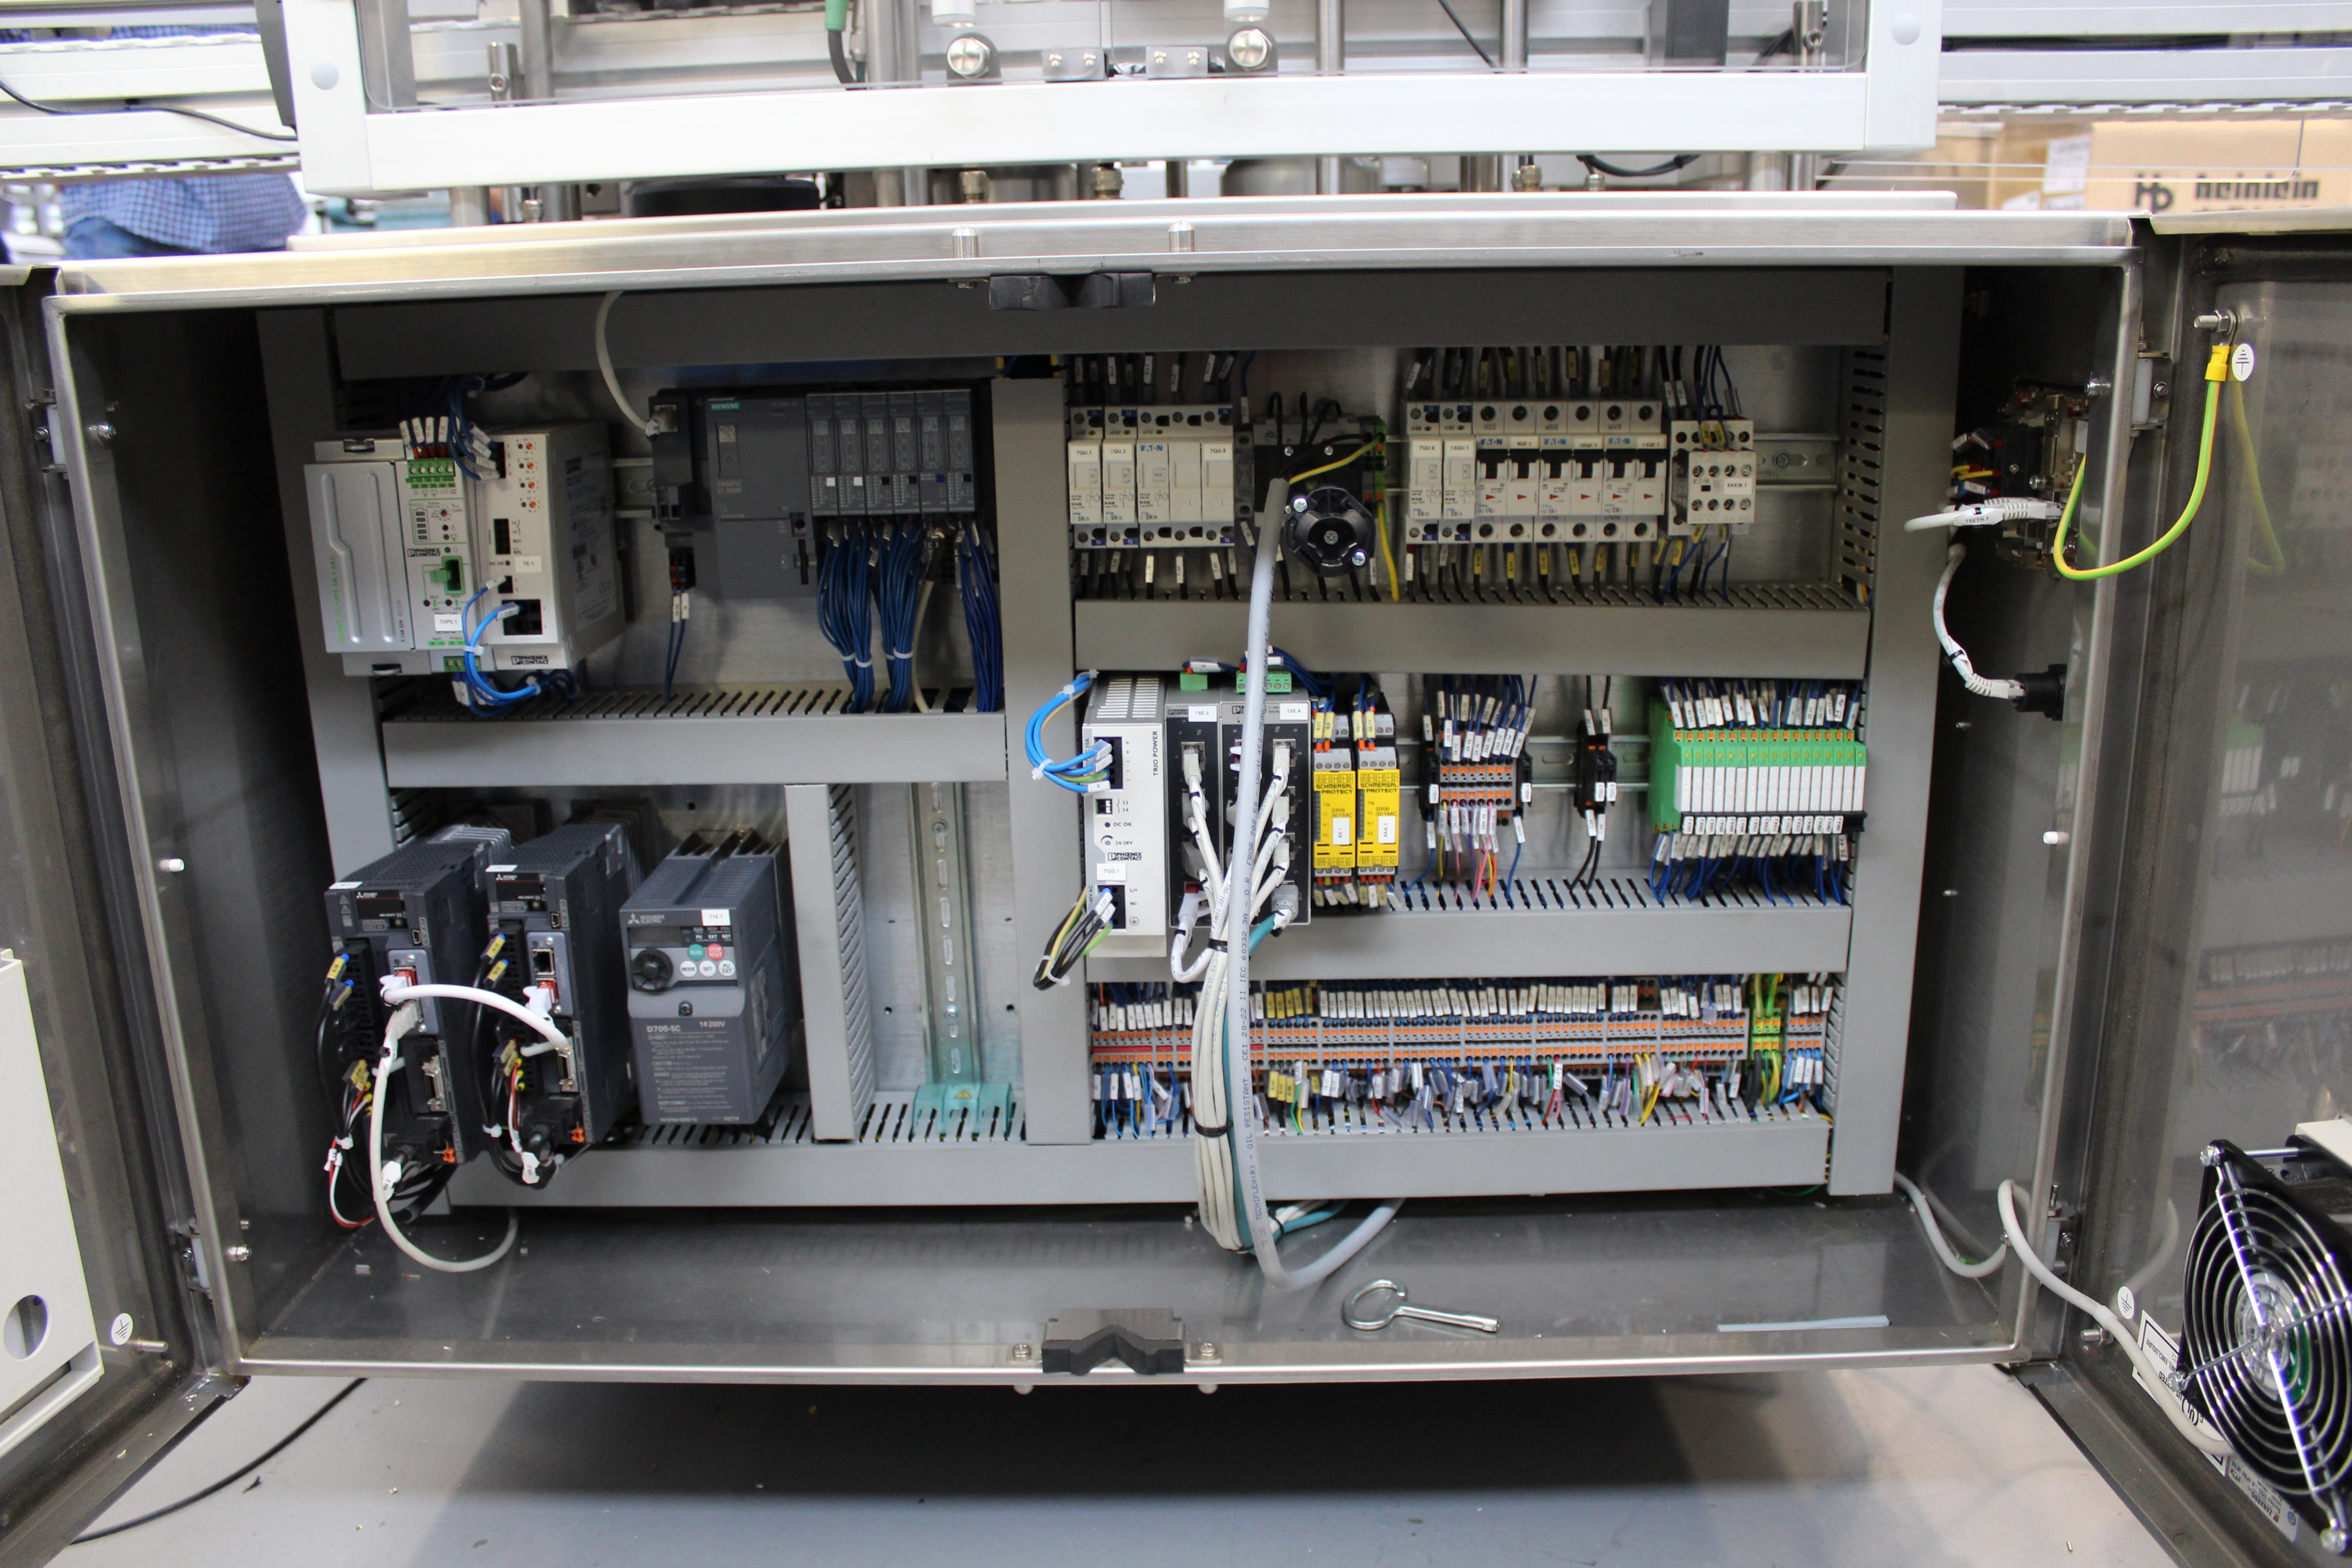
\includegraphics[width=12cm]{Immagini/ELE10}
	\label{ele10}
	\caption{Quadro Elettrico Completo}
	\end{figure}

\section{Funzionamento del Macchinario}
Prima di spiegare il funzionamento dettagliato del macchinario, conviene introdurre brevemente il suo funzionamento base. Per maggiore chiarezza il processo di etichettaggio verrà descritto a fasi.
\\
Il funzionamento base del macchinario è abbastanza semplice. 
	\begin{itemize}
	\item \textit{Ingresso Flaconi:} all ingresso all' etichettatrice abbiamo un nastro trasportatore che arriva dalla macchina precedente, che nel caso di questa linea è una macchina riempitrice.
	\item \textit{Controllo Presenza:}  i flaconi uscenti dalla riempitrice scorrono sul nastro fino al raggiungimento della prima stella. Durante il trasporto nella prima stella, ogni flacone viene rilevato dal sensore di presenza prodotto.
	\item \textit{Etichettatura:} successivamente il flacone viene agganciato dalla seconda stella che lo trasporta sull'unità di etichettaggio. Quando il flacone si trova in prossimità della 'pinna', viene attivata la testa di etichettatura che effettuerà l'applicazione.
	\item \textit{Massaggio:} quasi istantaneamente all'applicazione, il flacone rotola su un nastro detto massaggiatore che assicura una corretta applicazione dell'etichetta.
	\item \textit{Uscita Flacone:} a questo punto il flacone viene agganciato dalla terza ed ultima stella che lo trasporta sul nastro di uscita verso la macchina a valle. 
	\end{itemize}

Avendo sommariamente illustrato il funzionamento base della nostra etichettatrice tralasciando controlli, sistemi di visione, meccanismi di scarto ed altro, andiamo ora a spiegare un po più nel dettaglio cosa avviene realmente in ogni fase.

\subsection{Ingresso Flaconi}
Nella fase di ingresso flaconi, come si può ben immaginare, non vi è solo un semplice nastro che trasporta i flaconi da un punto ad un altro, bensì vi sono alcuni controlli necessari per un corretto funzionamento del macchinario, nonchè di protezione del sistema stesso. Il nastro in ingresso è regolabile in velocità mediante un inverter per assicurare che i flaconi arrivino con una giusta frequenza. 

	\begin{figure}[H]
	\centering
	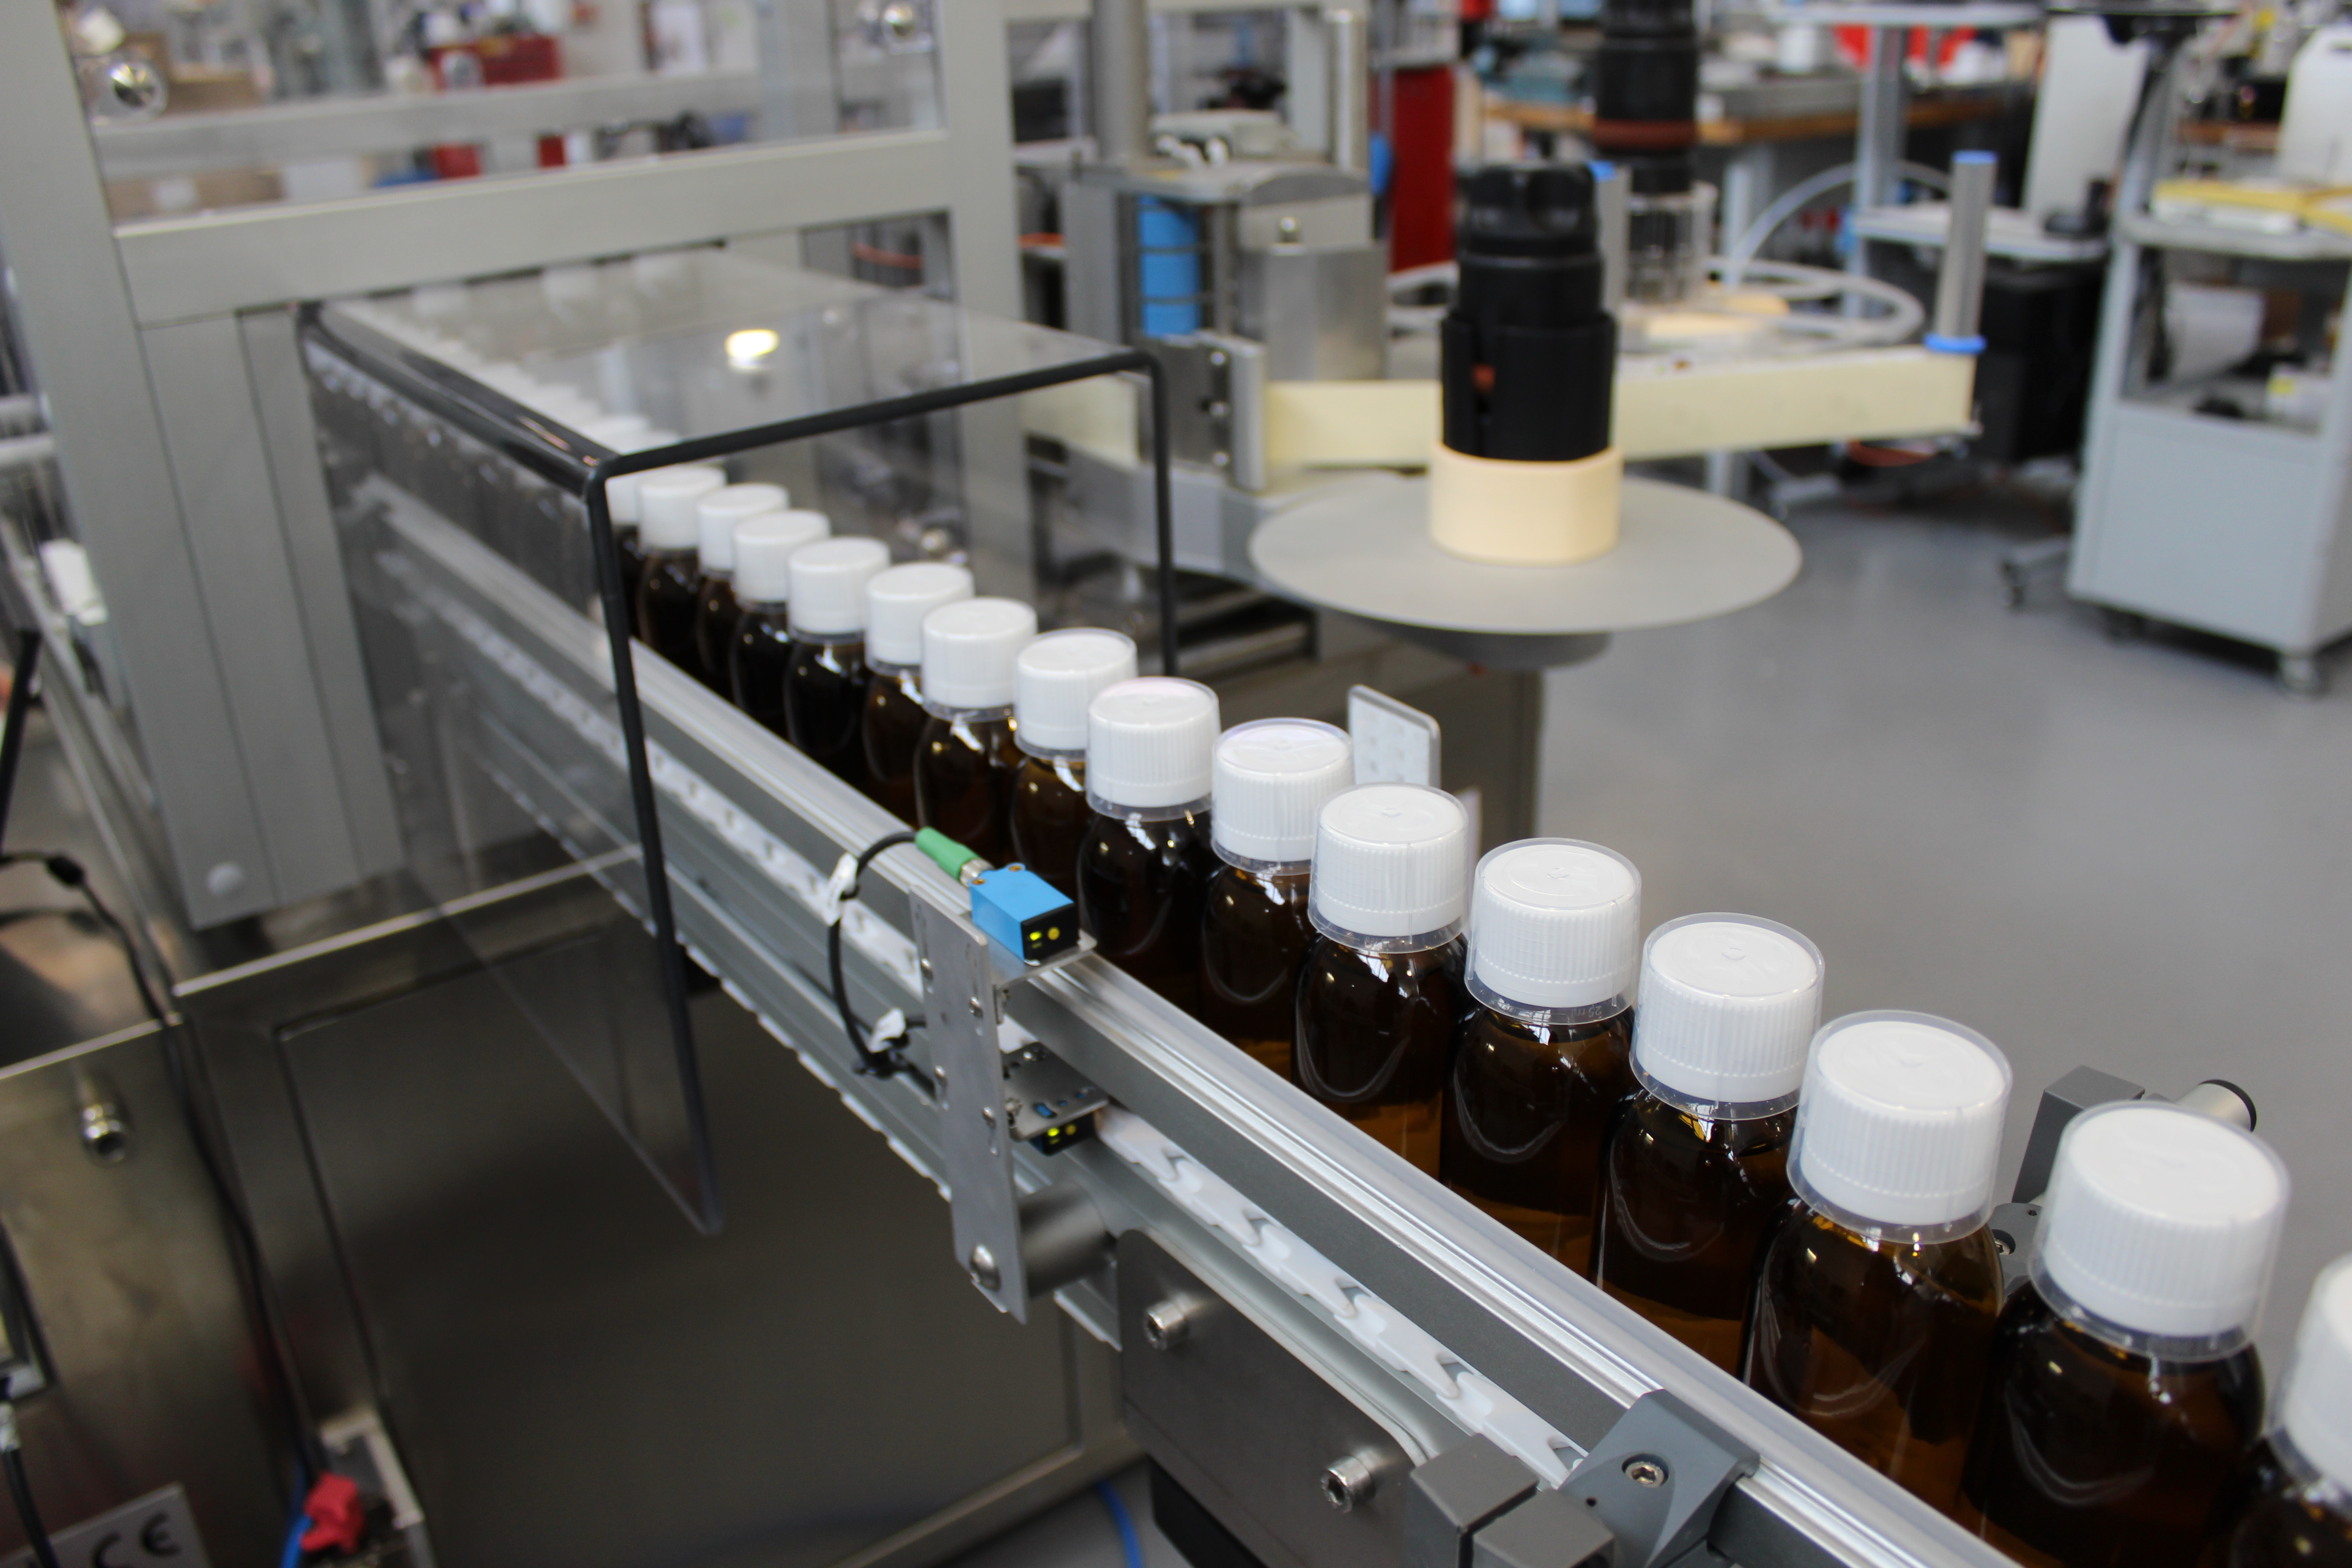
\includegraphics[width=12cm]{Immagini/MEC3}
	\label{mec3}
	\caption{ Nastro in Ingresso}
	\end{figure}

Non manca sul nastro in ingresso il sensore di minimo carico che segnala il plc qualora non ci sia prodotto. Alla ricezione di tale segnale il plc provvederà a fermare la macchina che altrimenti girerebbe inutilmente (vi sono inoltre anche segnali di abilitazione che arrivano dalla macchina a monte, necessari a segnalare un interruzione della linea).
Un problema da non sottovalutare nella nostra applicazione è la possibilità che un flacone si rovesci su nastro o arrivi già rovesciato dalla macchina a monte. Un flacone rovesciato potrebbe essere estremamente pericoloso: se la stella alla fine del nastro dovesse agganciare un flacone di vetro mal posizionato lo farebbe in mille pezzi e rischierebbe di danneggiare la macchina. Per evitare ciò, abbiamo munito il minimo carico di doppio sensore (uno alto ed uno basso). 

	\begin{figure}[H]
	\centering
	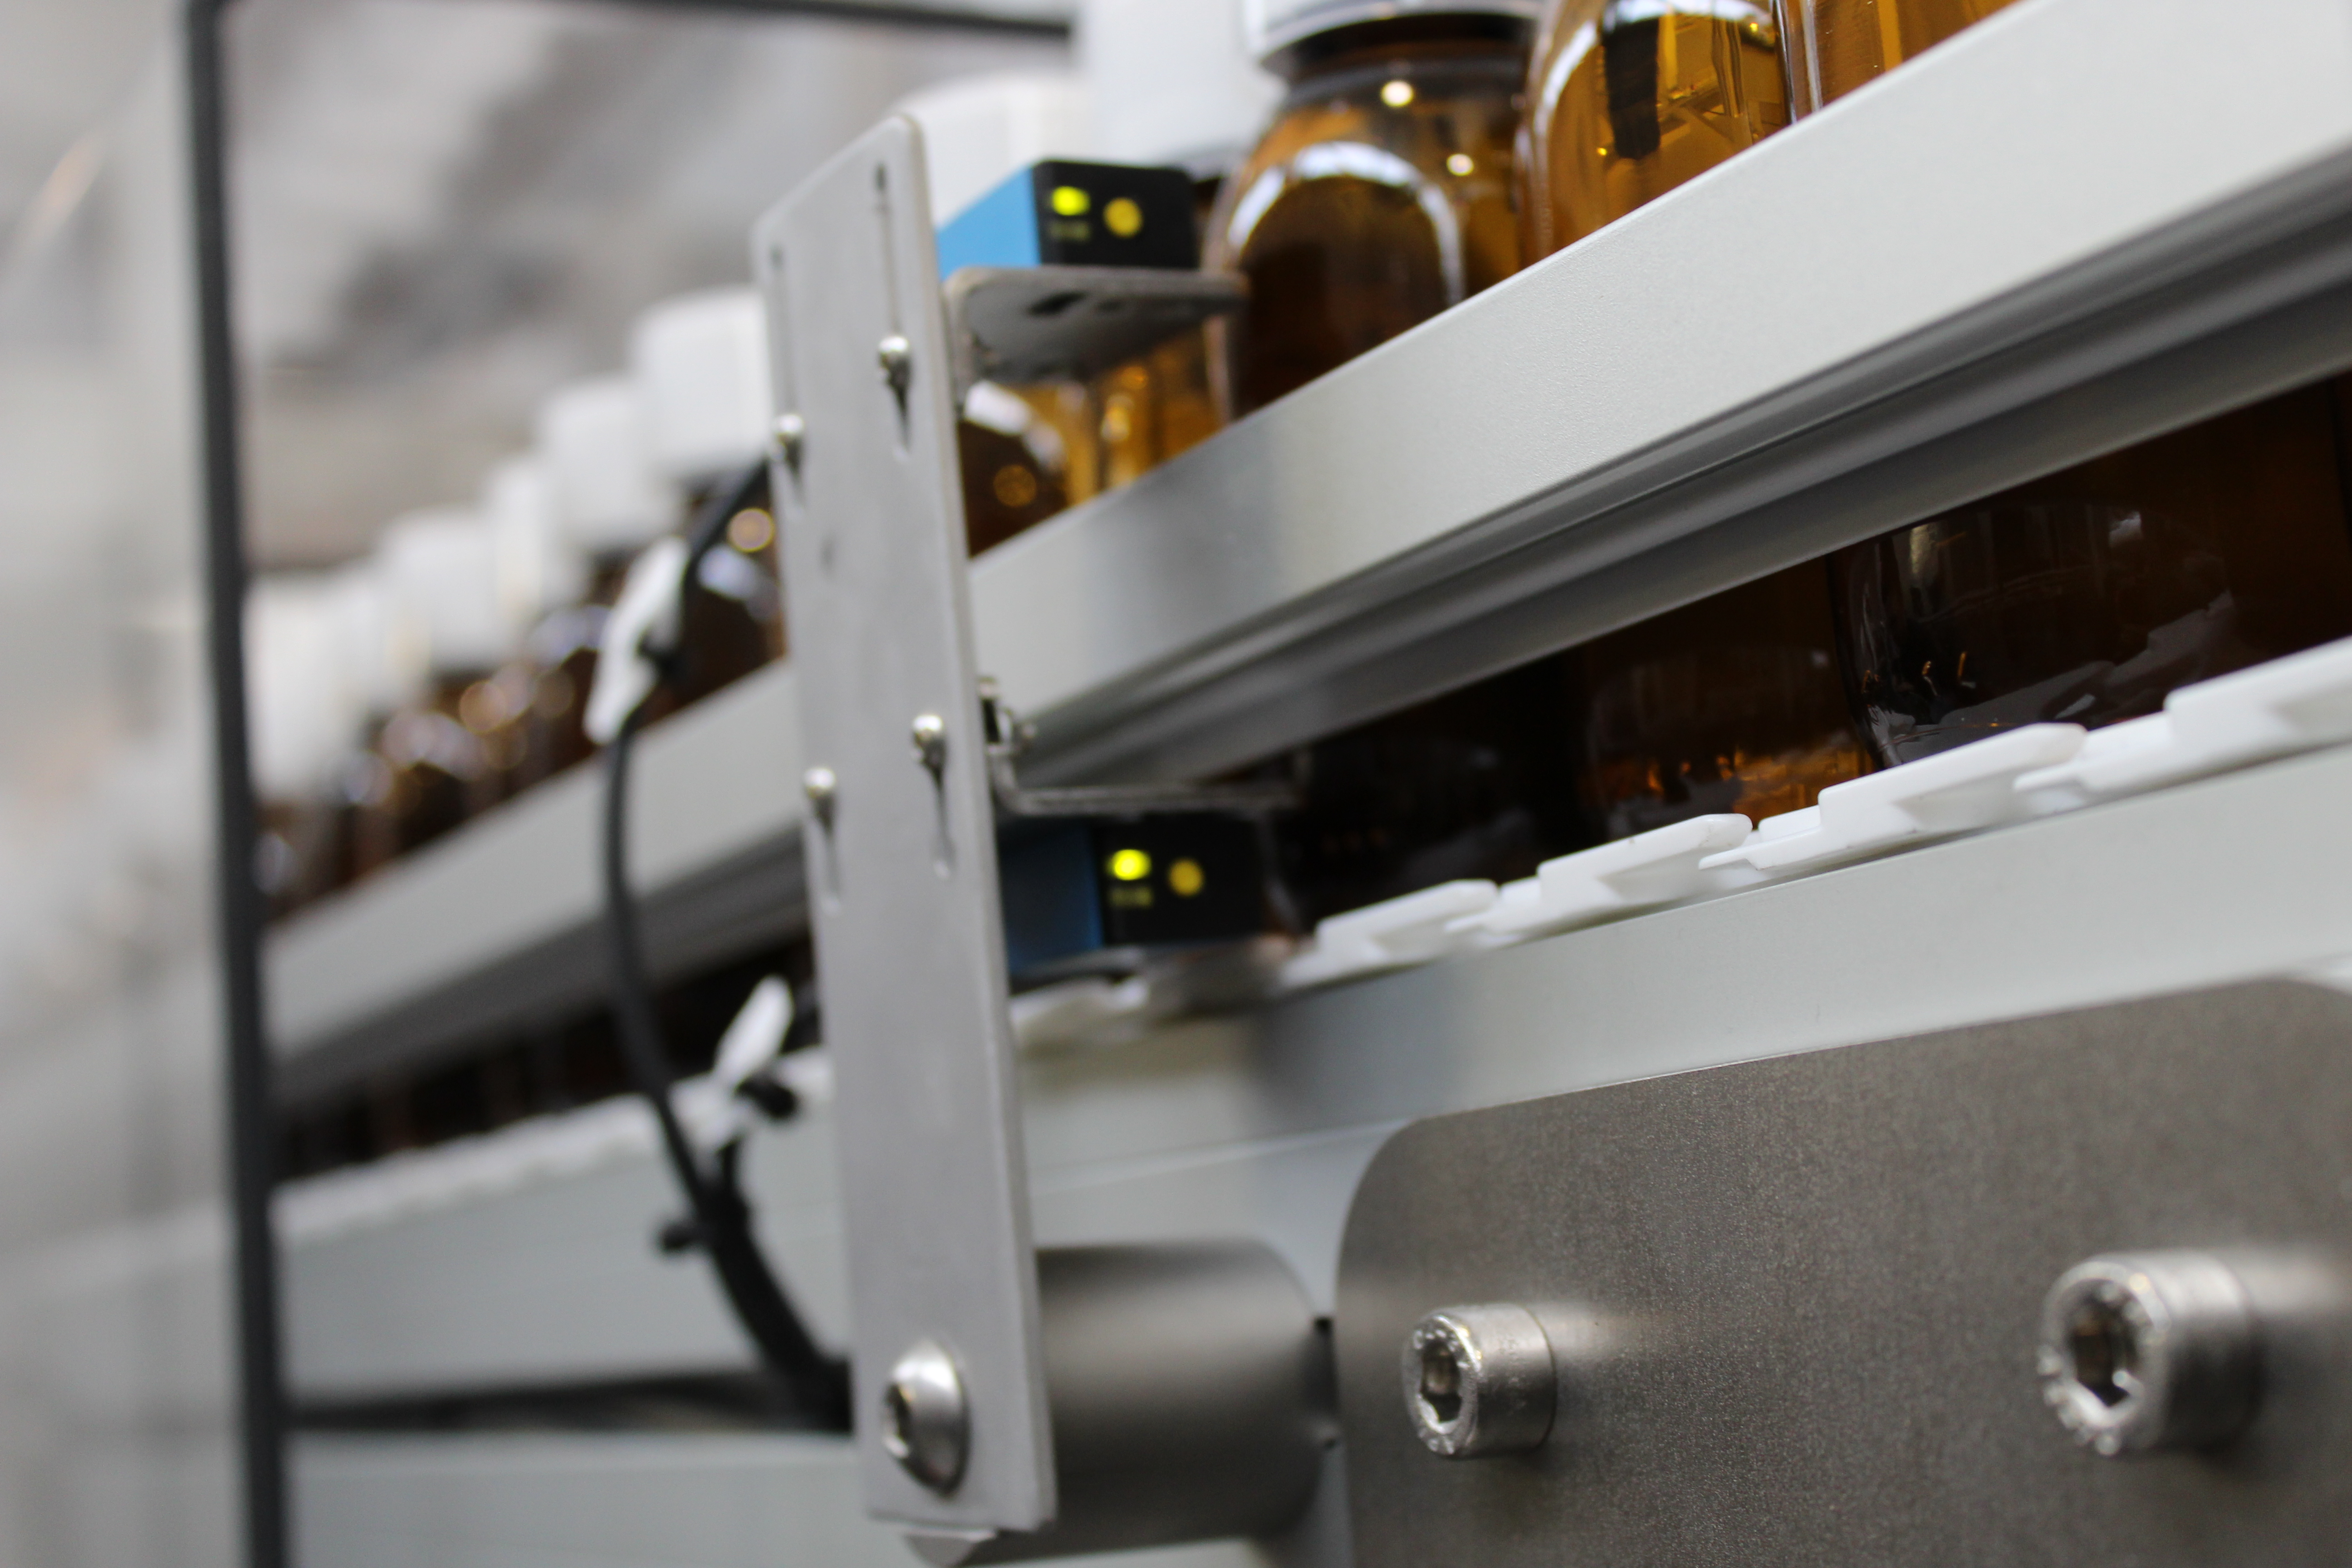
\includegraphics[width=12cm]{Immagini/MEC4}
	\label{mec4}
	\caption{ Doppio Sensore Carico Minimo ed anti rovesciamento flacone}
	\end{figure}

Questi due sensori lavorano in contemporanea uno sopra l'altro, in modo che se un flacone dovesse passare rovesciato, solo il sensore basso ne rileverebbe la presenza. Questa situazione manda un allarme che blocca immediatamente la macchina avvisando l'operatore con una segnalazione sul pannello operatore e mediante il torrino luminoso.  
   
\subsection{Controllo Presenza}
In questa fase, che sembra la più banale, inizia il momento decisivo del controllo che si porterà avanti per tutto il processo. Il flacone viene agganciato dalla prima stella e durante il trasporto il sensore di presenza ne verifica la presenza. 

	\begin{figure}[H]
	\centering
	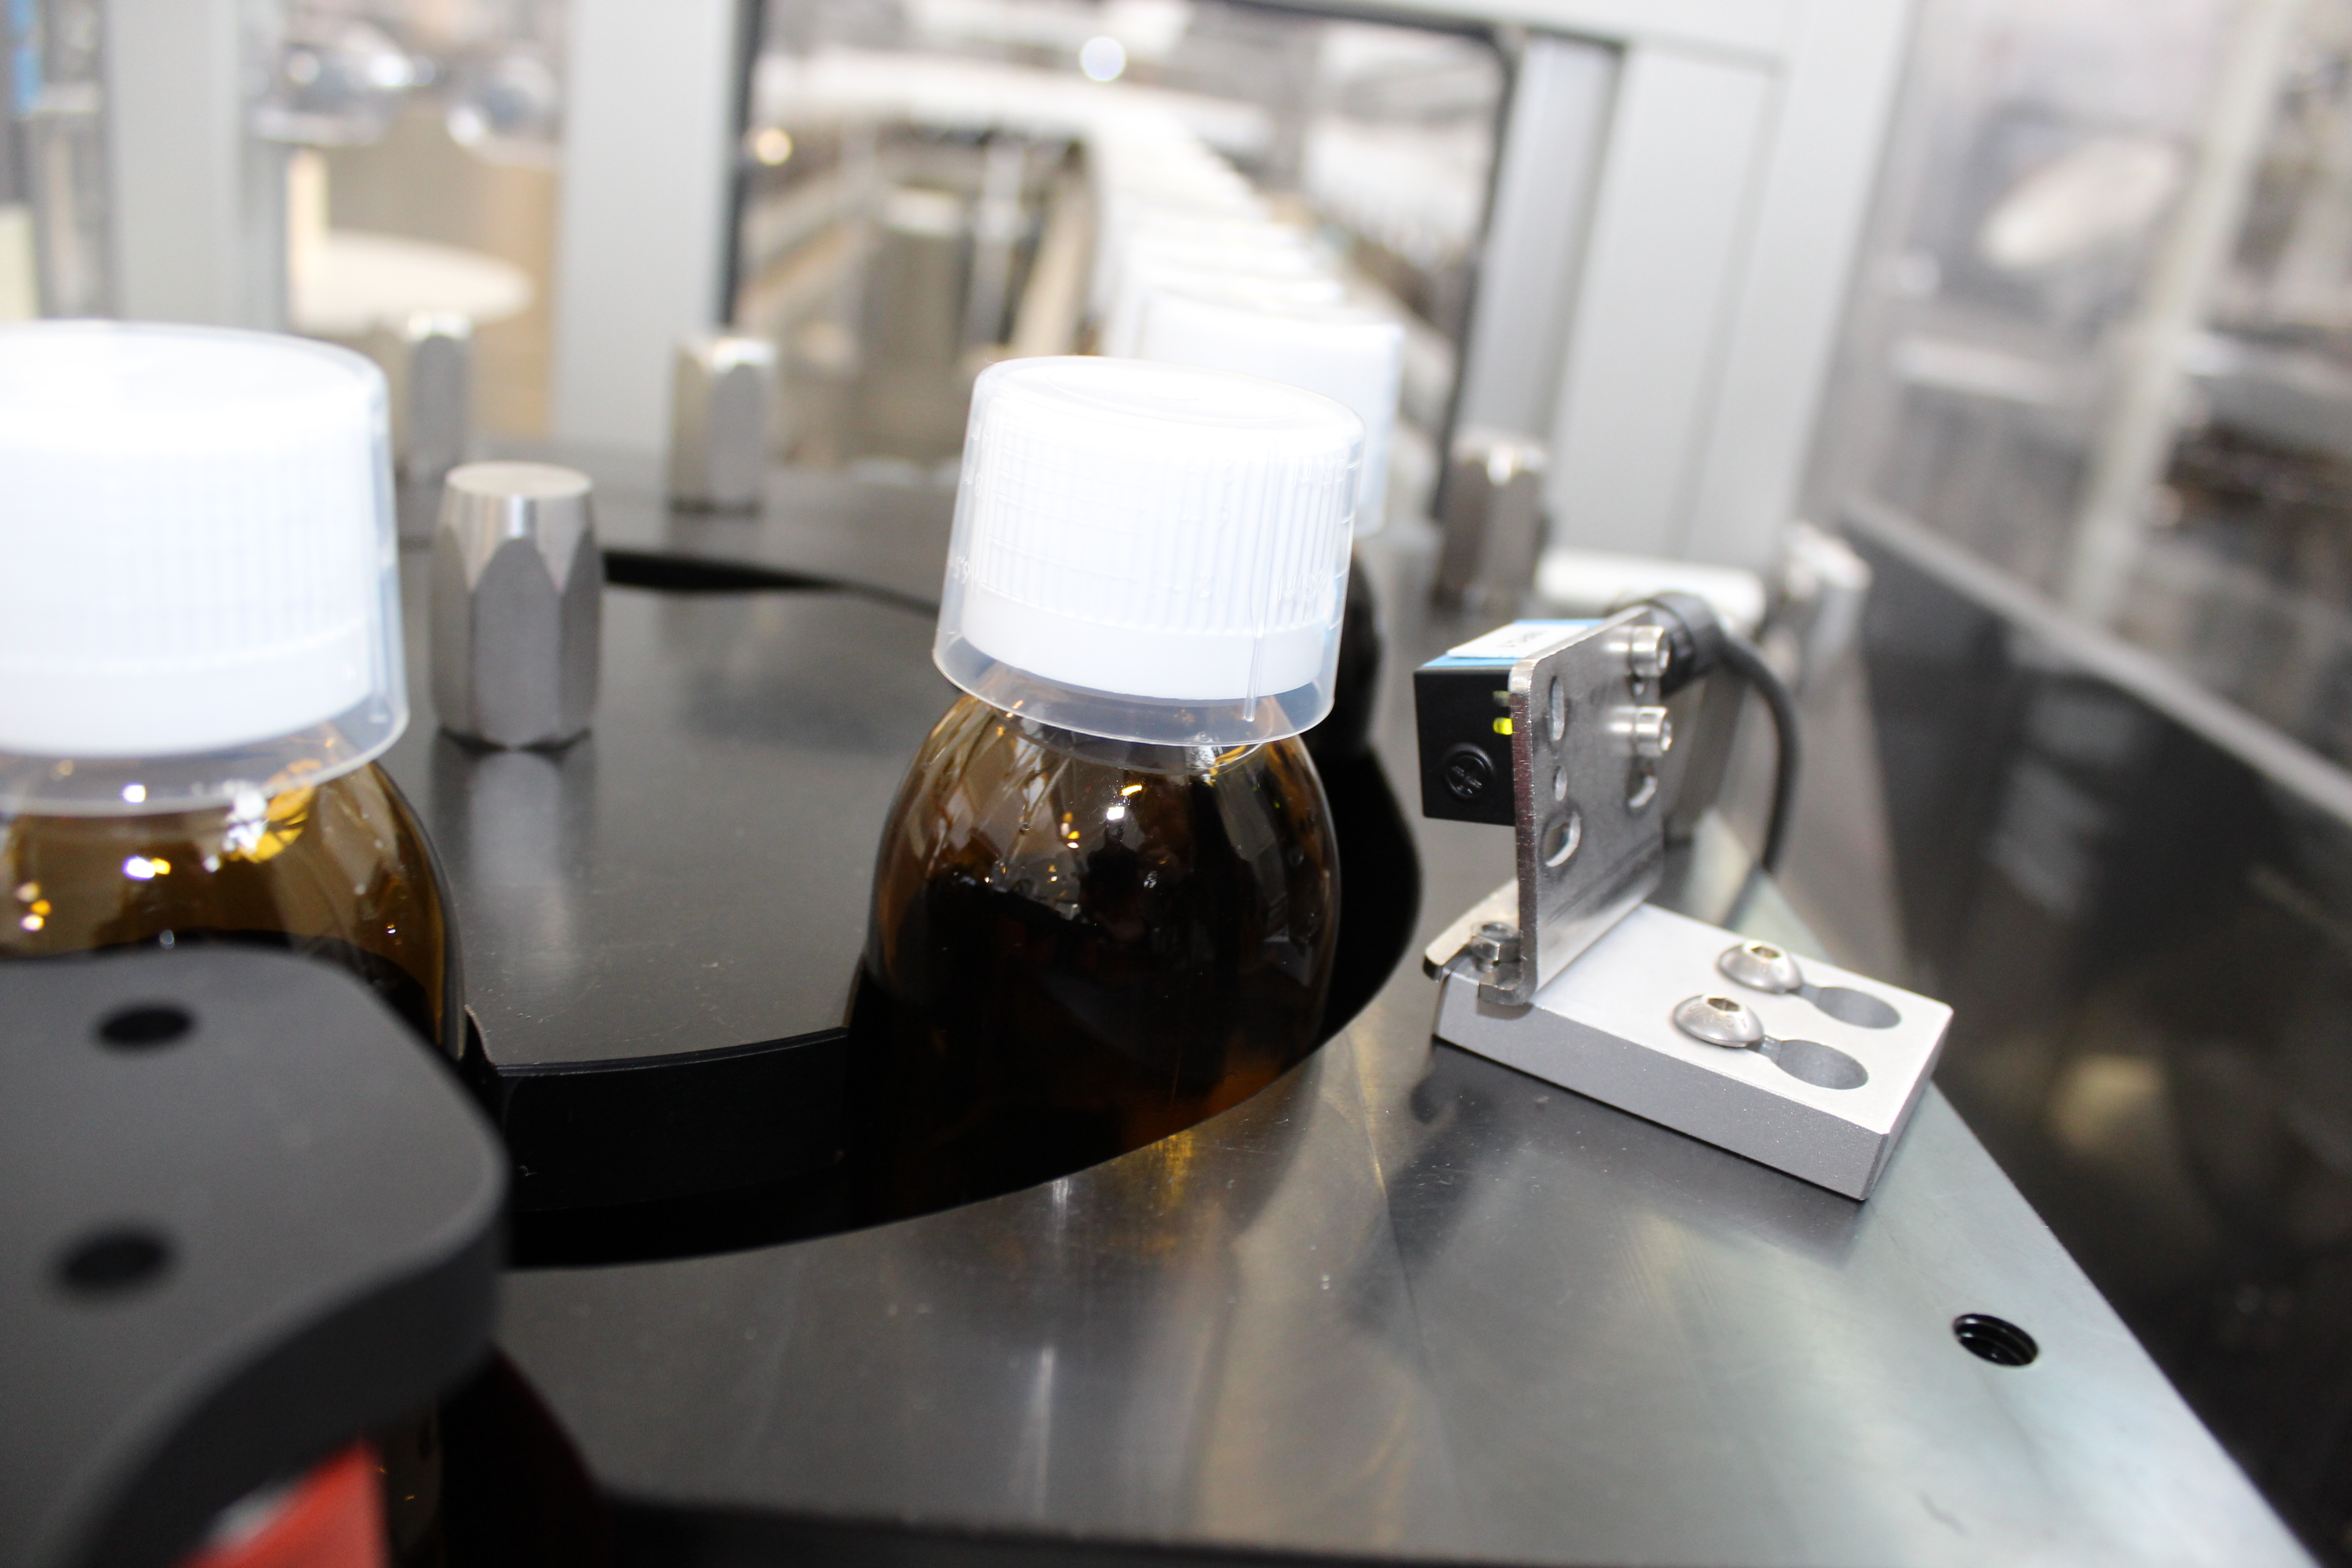
\includegraphics[width=12cm]{Immagini/MEC5}
	\label{mec5}
	\caption{ Sensore presenza flacone stella ingresso}
	\end{figure}

Questo momento è cruciale perchè è quì che si attiva lo 'Shift Register' del controllo che vedremo in dettaglio nei capitoli successivi. Per ora anticipiamo lo 'Shift Register' come l'elemento che ci permette di determinare la posizione e lo stato di ogni flacone all'interno della macchina.


\subsection{Etichettatura}
Sicuramente una delle fasi più importanti di tutto il processo, l'etichettatura è anche la più complessa a livello di controlli e settaggio. Il flacone, una volta rilevato dal sensore di presenza, viene agganciato dalla seconda stella che lo trasporta sulla pinna di etichettatura. Una volta che esso si trova in prossimità della pinna, viene inviato un comando di trigger digitale alla testa di etichettatura che espellerà l'etichetta. 

\begin{figure}[H]
	\centering
	\includegraphics[width=12cm]{Immagini/MEC6}
	\label{mec6}
	\caption{ Zona di applicazione etichetta }
\end{figure}

\subsection{Massaggio}
Come precedentemente anticipato, il massaggio avviene nella fase immediatamente successiva all'applicazione etichette. Il massaggiatore, come si evince dalla figura \ref{MEC7}, massaggia l'etichetta sul flacone per assicurarne l'adesione. Per ottimizzarne l'adesione, ci si deve assicurare che la velocità con la quale viene applicata l'etichetta sia pressocchè simile a quella di rotolamento del flacone. Per questo motivo abbiamo munito il massaggiatore di un encoder (1) che comunica all'unità di etichettatura l'attuale velocità lineare del nastro affinchè regoli automaticamente la velocità di espulsione delle singole etichette.

\begin{figure}[H]
	\centering
	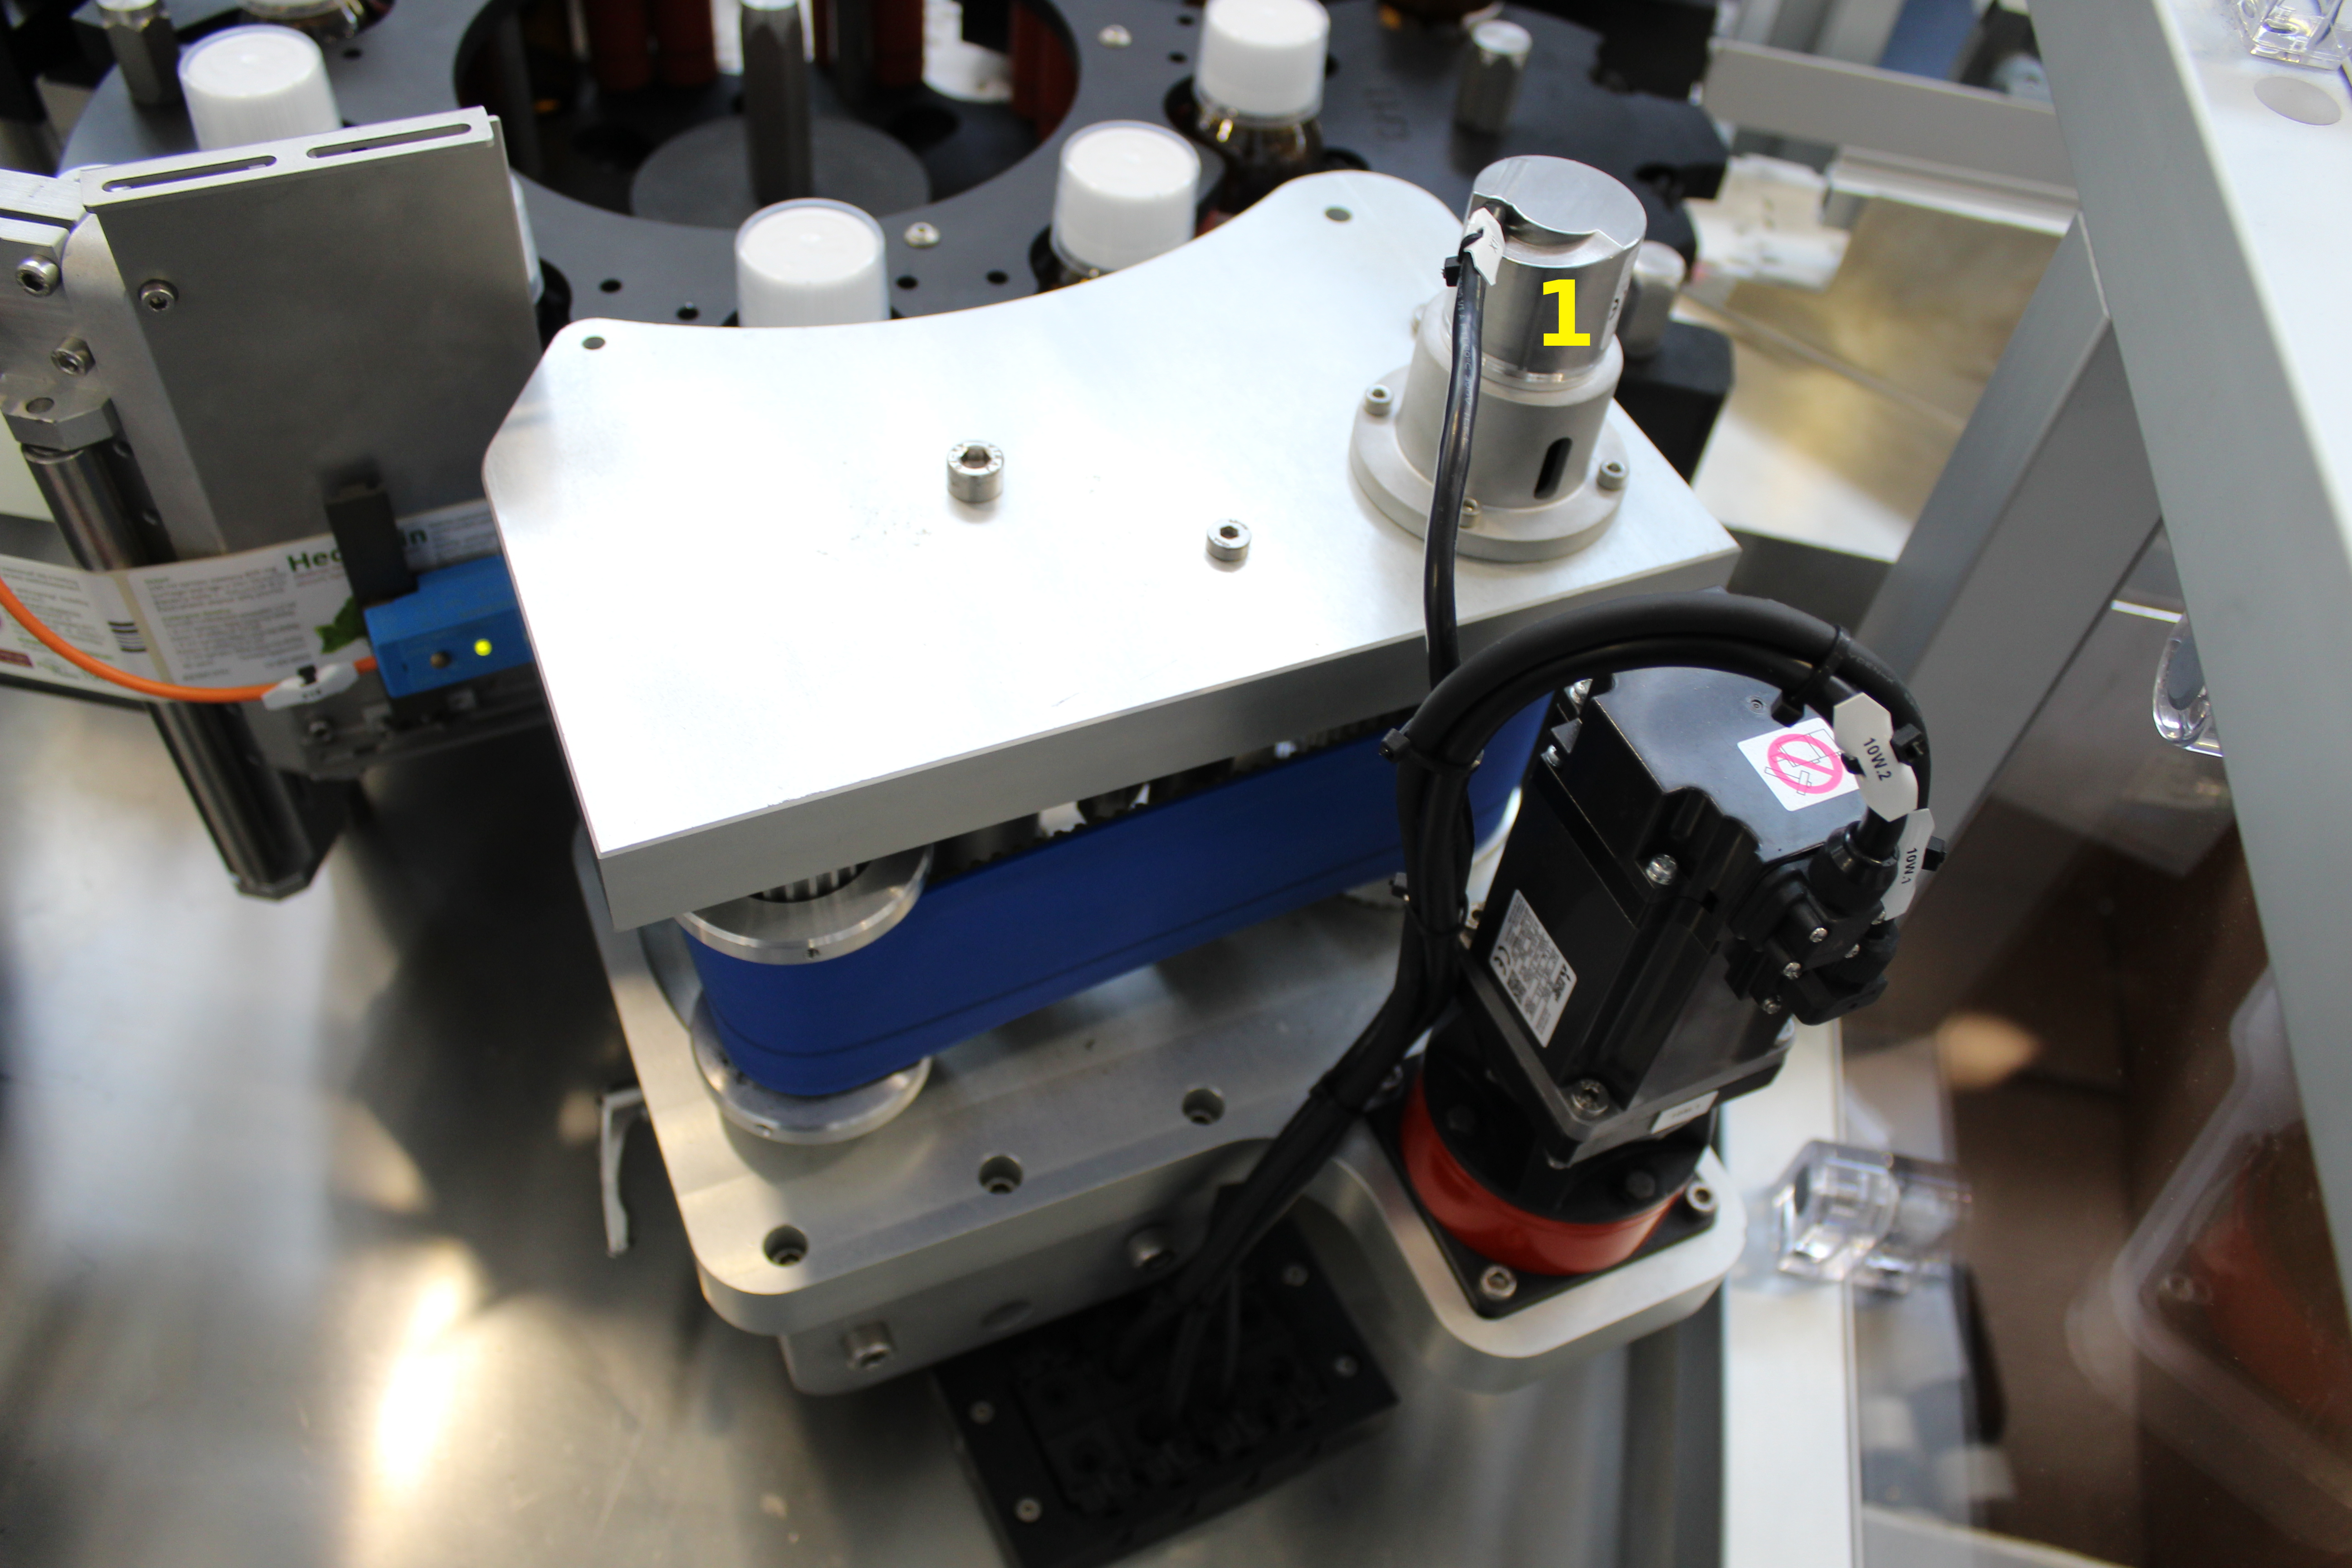
\includegraphics[width=12cm]{Immagini/MEC7}
	\label{MEC7}
	\caption{ Massaggiatore Etichette }
\end{figure}

\subsection{Uscita Flacone}
L'ultima fase del processo di etichettatura è quella di Uscita e Scarto. Dopo aver applicato l'etichetta e verificato la qualità del prodotto, spetta all'ultima stella decidere se rilasciare o meno il flacone sul nastro di uscita. Come accennato precedentemente, la stella di uscita possiede delle ventose ref{mec8} per catturare il flacone e dirigerlo verso il nastro oppure verso lo scarto, in base al risultato dei vari controlli effettuati durante il processo.

\begin{figure}[H]
	\centering
	\includegraphics[width=12cm]{Immagini/MEC8}
	\label{mec8}
	\caption{ Stella di Scarto }
\end{figure}

Nella figura possiamo notare come ciò avviene: nel caso di flacone non conforme rilevato dai sistemi di controllo, la stella di uscita che avrà agganciato precedentemente il flacone con il vuoto della specifica ventosa, invece di rilasciare il vuoto in prossimità del nastro, manterrà il flacone agganciato fino al raggungimento della zona di scarto. Raggiunta questa zona le ventose rilasciano automaticamente il vuoto lasciando cadere il flacone non conforme nel raccoglitore di scarto \ref{mec9}. 

\begin{figure}[H]
	\centering
	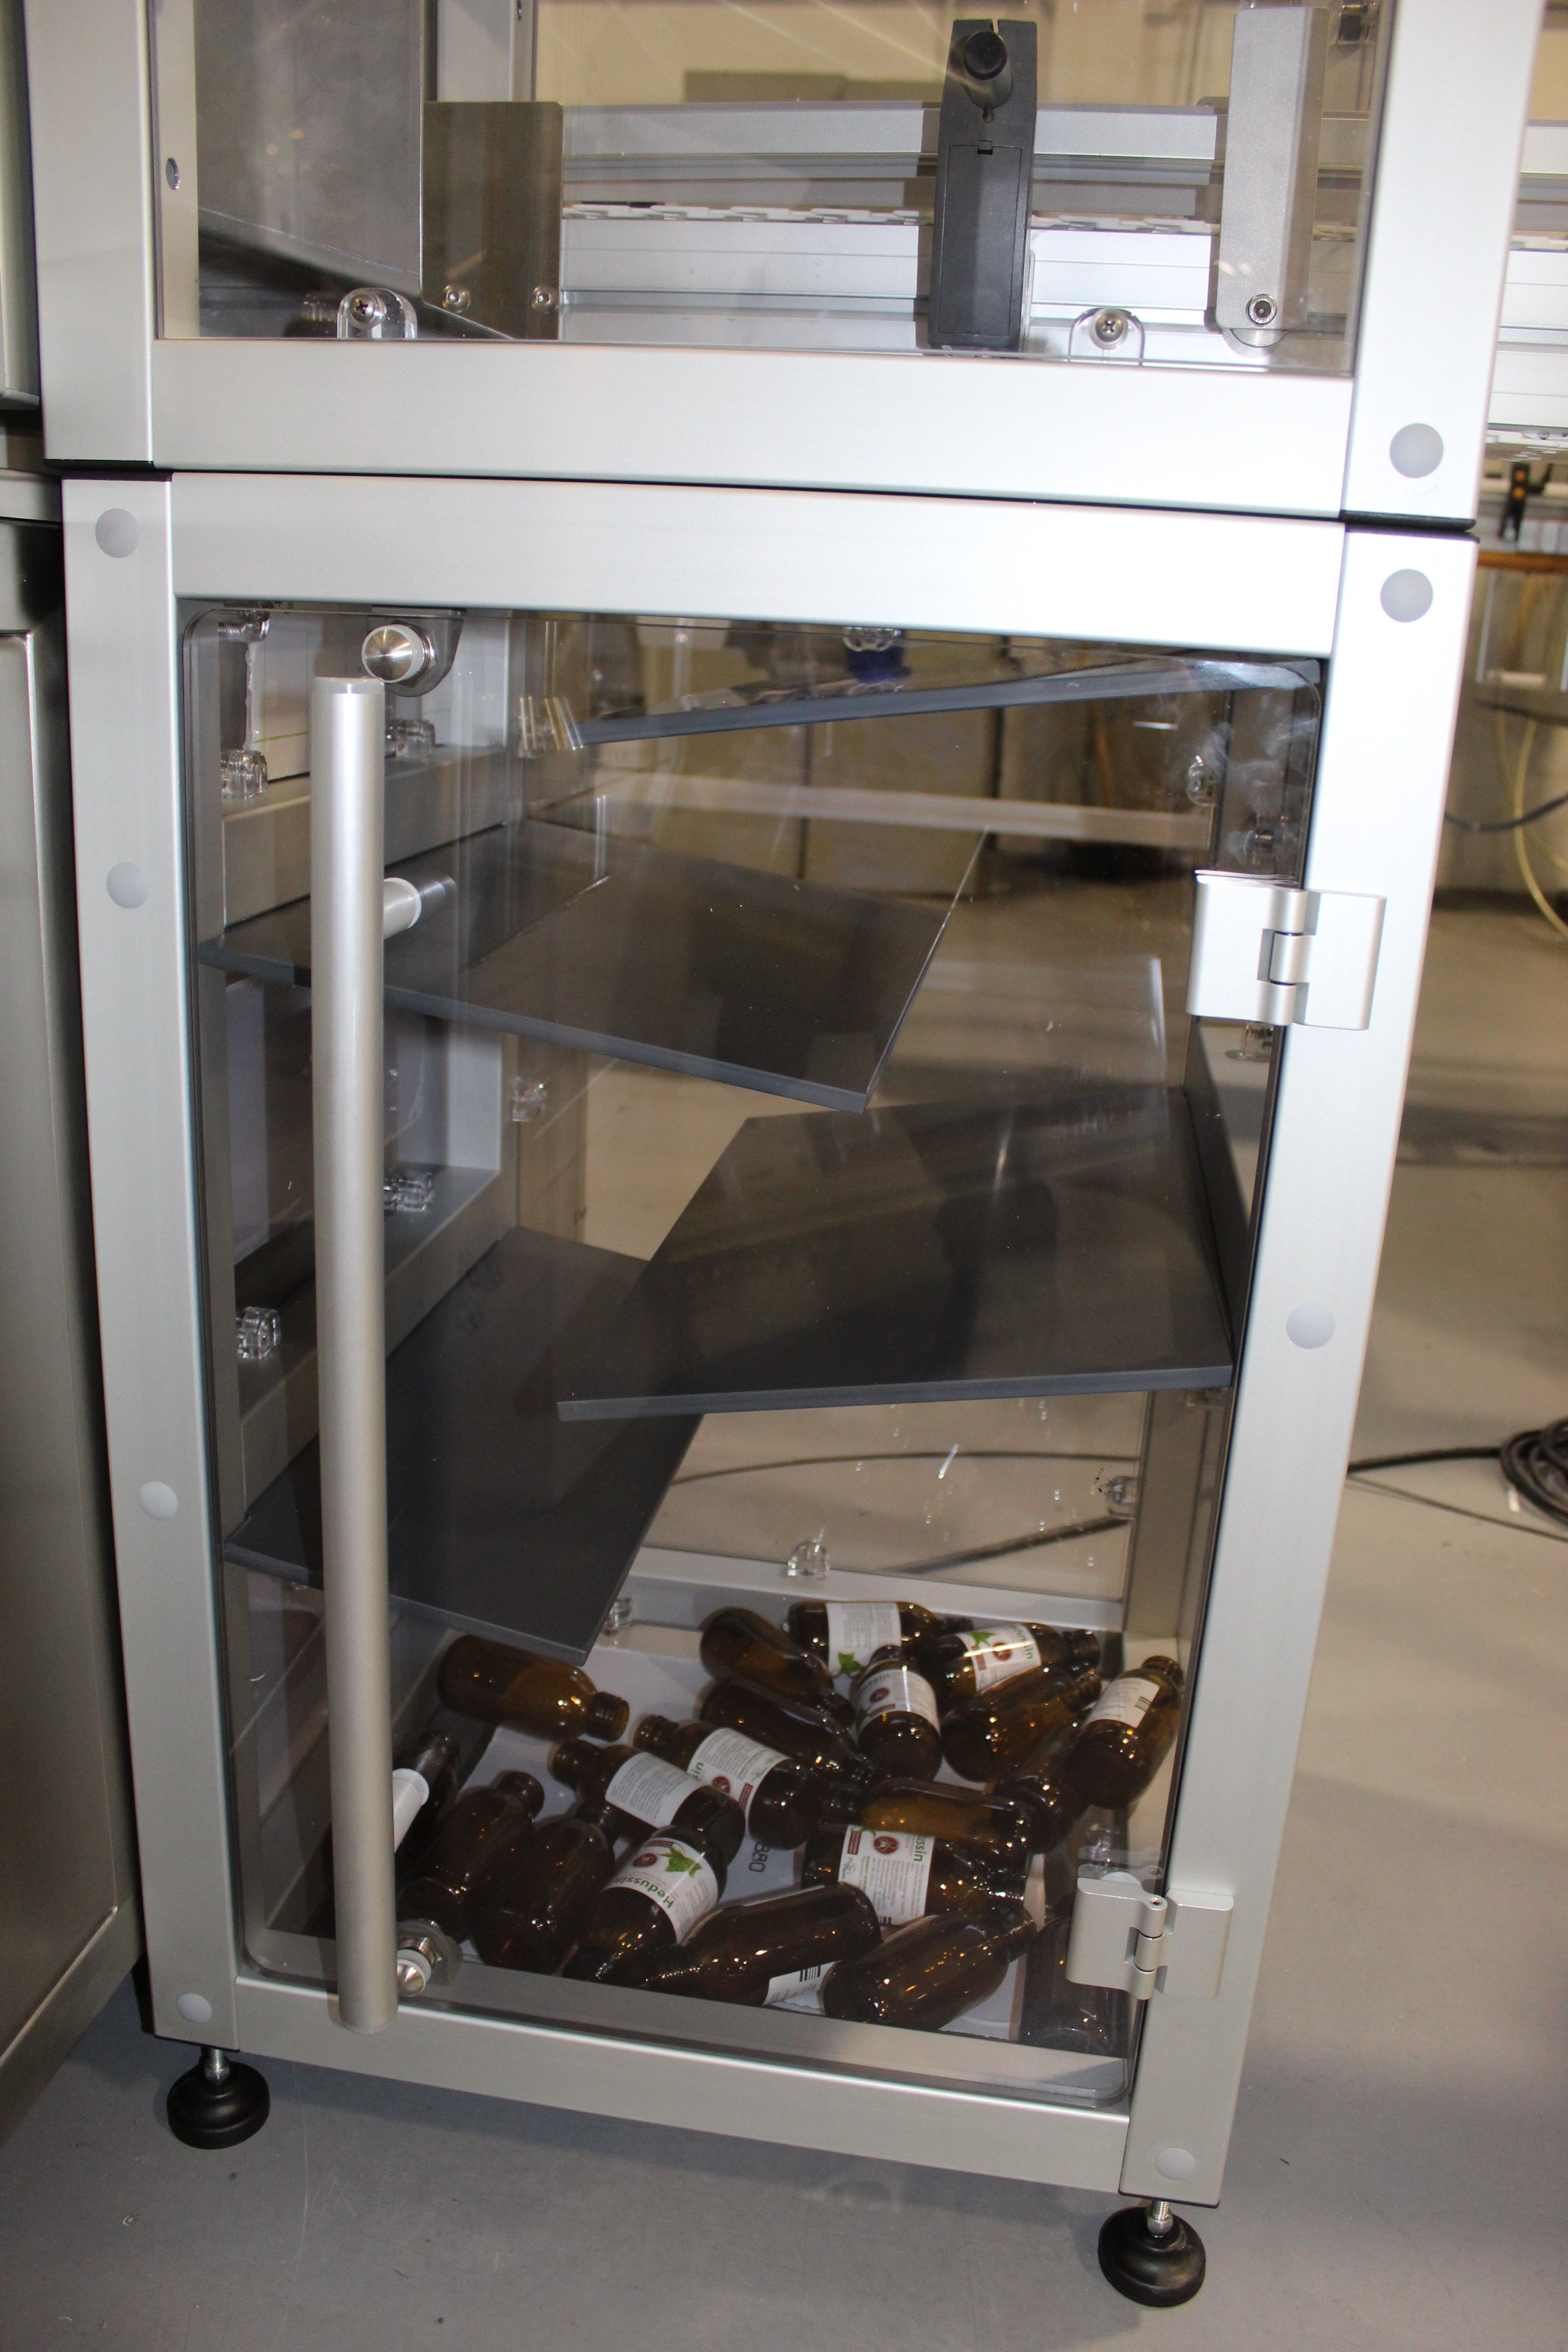
\includegraphics[width=12cm]{Immagini/MEC9}
	\label{mec9}
	\caption{ Raccoglitore di Scarto}
\end{figure}
 
\chapter{Processo di Sviluppo software PLC}
Un \textit{PLC} è, in pratica, un controllore programmabile, dotato di ingressi e uscite analogiche e digitali, con una o più connessioni di reti e specializzato nella gestione dei processi industriali. Il PLC esegue un programma ed elabora i segnali digitali ed analogici provenienti dai sensori ricevuti attraverso gli ingressi, generando sulle proprie uscite i corrispondenti comandi per gli attuatori presenti in un impianto industriale, i quali riescono a gestire una moltitudine di funzioni dalla più elementare (rilevare la temperatura, accendere una lampadina, etc) alle più sofisticate e complesse (muovere un braccio meccanico, programmare l'accensione/avviamento di macchine, automi, ecc). 
I PLC sono di solito istallati in armadi nelle vicinanze dell'impianto o direttamente a bordo della macchina. Gli I/O possono essere remoti: in questo caso sono collegati a morsettiere che vengono messe in comunicazione con il PLC mediante 'bus di campo' o anche direttamente su Ethernet. Sono necessarie postazioni utilizzate dagli operatori per 'vedere' e capire cosa succede negli impianti, dato che i PLC sono dei dispositivi 'ciechi' non dotati di interfaccia di visualizzazione.
\\La prima azione che il PLC compie è la lettura degli ingressi del portale e si intende tutti gli ingressi sia digitali sia analogici, on board o su bus di campo (schede remote collegate al PLC o con una rete di comunicazione). Dopo aver letto tutti gli ingressi, il loro stato viene memorizzato in una memoria che è definita '\textit{Registro immagine degli ingressi}'. A questo punto le istruzioni di comando vengono elaborate in sequenza dalla CPU e il risultato viene memorizzato nel '\textit{Registro immagine delle uscite}'. Infine, il contenuto dell'immagine delle uscite viene scritto sulle uscite fisiche, ovvero le uscite vengono attivate. Poiché l'elaborazione delle istruzioni si ripete continuamente, si parla di elaborazione ciclica; il tempo che il controllore impiega per una singola elaborazione viene detto tempo di ciclo (solitamente da 10 a 100 millisecondi).
\section{Fase Iniziale }
Nella Fase iniziale dello sviluppo di un software PLC bisogna innanzitutto conoscere molto bene l'intero processo della macchina. In questa fase si studia la macchina a partire dai requisiti richiesti dal cliente. Vi è un lungo confronto tra i vari team di sviluppo Meccanico, Elettrico e Informatico per cercare di minimizzare l'errore. Il programmatore PLC solitamente entra in gioco quando il processo macchina è già ben definito e pertanto si conoscono già quasi tutti i sensori della macchina, i comandi in uscita ecc. 
Tutte queste informazioni sono riportate sullo Schema Elettrico della macchina.

\begin{figure}[H]
	\centering
	\includegraphics[width=12cm]{Immagini/SCELE1}
	\label{scele1}
	\caption{Schema di collegamento elettrico generale relativo al PLC ed ai moduli }
\end{figure}


Con lo schema elettrico il programatore può già incominciare a configurare il PLC definendo le variabili di Input Output sui vari moduli I/O. 

\begin{figure}[H]
	\centering
	\includegraphics[width=12cm]{Immagini/SCELE2}
	\label{scele2}
	\caption{Schema del primo Byte di Ingressi Del Secondo Modulo I/O}
\end{figure}

\begin{figure}[H]
	\centering
	\includegraphics[width=12cm]{Immagini/SCELE3}
	\label{scele3}
	\caption{Schema elettrico relativo alle Uscite del Modulo Analogico }
\end{figure}

\subsection{Configurazione Iniziale con TiaPortal v13}
	Avendo PLC Siemens, naturalmente il software utilizzato è TiaPortal nello specifico la versione 13.
	TiaPortal consente molto agevolmente di creare l'architettura della macchina slezionando i componenti da un catalogo interno. I vari componenti Hardware possono essere ricercati tramite codice identificativo riportato sul componente stesso oppure tramite metodo di autoapprendimento via Profinet. Al termine della configurazione PLC con i vari Moduli I/O la vista di rete di TiaPortal risulta la seguente.
	
	\begin{figure}[H]
		\centering
		\includegraphics[width=12cm]{Immagini/TIA0}
		\label{tia0}
		\caption{Configurazione Tia Portal del Rack PLC}
	\end{figure}


	Una volta importati vari componenti del rack PLC, si possono definire ed impostare le variabili I/O in modo da risultare coerente con lo schema elettrico della macchina.
	
	Finita la procedura di configurazione del rack PLC si può passare all'aggiunta dei vari componenti Profinet della macchina. \\
	Ricordiamo che i componenti compatibili Profinet della nostra etichettatrice sono:
	\begin{itemize}
		\item Azionamento Mitsubishi Motore Principale
		\item Azionamento Mitsubishi Motore Massaggiatore
		\item Telecamera Datalogic Contollo Etichetta
		\item Telecamera Datalogic Controllo Allineamento
		\item Encoder Sick Assoluto
	\end{itemize}

	Per poter importare un componente Profinet-Compatible su TiaPortal necessitiamo di un GSD (General Station Description). I file GSD rappresentano un file formattato in XML, fornito dal produttore, che descrive il componente in termini di caratteristiche di comunicazione, struttura dei dati di ingresso ed uscita, diagnostica, parametri di impostazione. Tramite il GSD, TiaPortal potrà sapere come comunicare con il Registro del dispositivo e pertanto ricevere ed inviare informazioni ad esso. Il GSD tuttavia non da un'interfaccia sui comandi inviabili o dati ricevibili dal dispositivo, questo task spetta al programmatore che deve studiare la comunicazione Profinet di ogni signolo dispositivo e scoprire su quali registri scrivere (per inviare comandi) o leggere (per ricevere informazioni). I dettagli sulle comunicazoni Profinet dei vari dispositivi verranno visti nel capitolo \cite{profinet}
	Una volta importati i GSD dei vari dispositivi TiaPortal ne mappa i registri in variabili di Memoria Locale al PLC in modo da semplificarne l'accesso. 
	

	\begin{figure}[H]
		\centering
		\includegraphics[width=12cm]{Immagini/TIA1}
		\label{tia1}
		\caption{Mapping Variabili GSD Motore Mitsubishi. Il Custom Telegram del GSD Mappa gli ingressi dei registri dell'azionamento sulle variabili I-600 alla I-647 e lo stesso per le uscite rispettivamente Q-600 a Q-647}
	\end{figure}

	
	Tutti i dispositivi profinet inoltre devono avere un indirizzo di rete univoco ed essere nella stessa SubNet. Gli indirizzi di rete sono configurabili in TiaPortal tramite un tool che rileva tutti i dispositivi direttamente connessi all Switch tramite un broadcast a Livello 2 che permette la visualizzazione di tutti gli indirizzi MAC dei dispositivi profinet connessi. A questo punto risulta molto semplice assegnare l'indirizzo IP a ciascun dispositivo.
	
	Con questo si può dare per conclusa la fase di inizializzazione del progetto software PLC

\section{Struttura Software PLC}

I sistemi di controllo si basano sul software per controllare il processo produttiva. Questo tipo di attivita si svolge per fasi, dopo la fase di raccolta delle informazioni si passa quella di progettazione, segue quella di implementazione. Come si può immaginare tale software deve soddisfare dei requisiti di qualità. Per qualità del software si intende la misura in cui un prodotto software soddisfa un certo numero di aspettative rispetto sia al suo funzionamento sia alla sua struttura interna. Gran parte della ricerca nel campo dell'ingegneria del software è dedicata direttamente o indirettamente, al tema della qualità del software. I fattori rispetto a cui misurare o definire la qualità sono le seguenti: 
\begin{itemize}
	\item \textit{Correttezza}: un programma o sistema si dice corretto se si comporta esattamente secondo quanto previsto dalla sua specifica dei requisiti,  se il comportamento del software e quello previsto dai progettisti.  
	\item \textit{Affidabilità}: un sistema e tanto più affidabile quanto più raramente si manifestano malfunzionamenti durante l'utilizzo del sistema, tenendo conto che, nella valutazione dell'affidabilità, errori gravi si considerano solitamente più influenti rispetto a errori non gravi, indipendentemente dalla frequenza con cui si manifestano.
	\item \textit{Robustezza}: è la misura di come il sistema si comporta in situazioni impreviste non contemplate dalle specifiche. 
	\item \textit{Efficenza}: un sistema e efficiente se usa le risorse, CPU, memoria, in modo efficiente ovvero in modo proporzionale al servizio che deve svolgere. Un sistema software non efficiente pregiudica le prestazioni di tutto il sistema di controllo.
	\item \textit{Manutenibilità}: facilità di apportare modifiche al sistema realizzato (è maggiore se il sistema è ben progettato),  non corrispondo solo alla correzione degli errori ma comprende anche l'evoluzione del software.
\end{itemize}

Come in tuti i processi di sviluppo del software,  arrivati alla fine della implementazione si passa alla fase di test e collaudo. Si collauda il software per verificare il comportamento e rilevare errori di programmazione, dopo di che si passa al collaudo del impianto di produzione (chiamata messa in servizio) testando il comportamento di tutto il sistema hardware/software. Anche questo processo di sviluppo produce la propria documentazione.

\subsection{Linguaggi di Programmazione}
I linguaggi utilizzati per la programmazione dei PLC sono generalmente linguaggi a basso livello. Come già accennato, alcuni produttori hanno scelto di dividere il codice e i dati in blocchi così da avere una separazione tra blocchi funzione FB e blocchi dati DB. Questo tipo di suddivisione del programma è molto efficace in quanto il programma è più comprensibile, una qualsiasi modifica viene fatta a livello di blocco sia esso di dati che di funzione. Dopo la stesura del codice il programma deve essere compilato prima di caricarlo nel PLC. Quindi in generale i linguaggi per la programmazione di PLC sono linguaggi compilati. Le norme IEC 1131-3 hanno avuto il merito di cercare di unificare i linguaggi di programmazione più diffusi nel mondo dei PLC, cercando di evitare il proliferare dei vari dialetti proposti dai diversi costruttori.
Questi linguaggi si dividono in due gruppi:

\begin{itemize}
	\item  Linguaggi Testuali 
		\begin{itemize}
			\item - ST: Structurated text
			\item - IL: Istruction list
		\end{itemize}
	\item Linguaggi Grafici
		\begin{itemize}
			\item - SFC: Sequential function chart
			\item - FBD: Function block diagram
			\item - LD: Ladder diagram
		\end{itemize}
\end{itemize}

Di seguito viene data una breve descrizione di questi linguaggi.

\subsubsection{Il linguaggio Structured Text}
Il linguaggio testuale Structured Text (ST) rappresenta il passaggio alla programmazione strutturata e di alto livello per i controllori industriali. Mantenendo la semplicità e la chiarezza sintattica necessarie per essere utilizzato con successo nello sviluppo di applicazioni anche complesse, può essere utilizzato su dispositivi dalle prestazioni computazionali limitate. Il linguaggio ST si presta per la risoluzione in modo rapido ed intuitivo di qualsiasi tipo di compito di programmazione. Tuttavia, dato il campo di applicazione ed il contesto nel quale è definito, considerando cioe anche gli altri linguaggi grafici o testuali della Norma IEC 61131-3, risulta particolarmente adatto per eseguire complesse elaborazioni matematiche, realizzabili con poche righe di codice, oppure nel caso in cui occorra eseguire test condizionali con molteplici alternative, i quali richiederebbero con la logica a contatti o con il linguaggio IL un grande numero di operazioni di salto con la conseguente riduzione di leggibilita del software sviluppato. Strutturalmente assomiglia al linguaggio Pascal. L'immagine in fig 2.13 riporta un esempio di questo linguaggio.

	\begin{figure}[H]
	\centering
	\includegraphics[width=8cm]{Immagini/SCL}
	\label{scl}
	\caption{Linguaggio SCL}
\end{figure}

\subsubsection{Il linguaggio Instruction List}
La tipica applicazione dei PLC industriali consiste nello svolgere compiti di controllo logico con operazione prevalentemente booleane e l'architettura hardware delle loro CPU è ottimizzata per svolgere questo tipo di operazioni in modo semplice e rapido. I linguaggi di livello assemblativo di tali dispositivi sono pertanto basati storicamente su una sintassi del tipo 1 operatore : 1 operando. Con questa sintassi, occorre un particolare tipo di registro interno del processore, detto accumulatore, nel quale memorizzare il risultato dell'operazione, mentre l'eventuale secondo operando necessario all'operazione (es. somma logica tra due valori booleani) consiste implicitamente nel contenuto dell'accumulatore stesso. Anche lo standard IEC 61131-3, essendo derivato dall'analisi dettagliata del panorama corrente del mercato PLC, segue questo tipo di sintassi per la definizione del linguaggio (Instruction List (IL), il linguaggio testuale di livello inferiore nello standard).
\\Essendo un linguaggio assemblativo, tutti gli altri linguaggi possono avere un'equivalente in IL, mentre non è sempre possibile convertire codice IL in altri linguaggi. Infatti, l'IL si presta per sua natura alla generazione di codice ottimizzato, il quale tuttavia potrebbe perdere l'equivalenza con codice di alto livello o diagrammi grafici in LD o FBD (trattati in seguito). 
L'immagine in fig \ref{IL} riporta un esempio di questo tipo di linguaggio.

	\begin{figure}[H]
	\centering
	\includegraphics[width=12cm]{Immagini/IL}
	\label{IL}
	\caption{Linguaggio IL}
\end{figure}



\subsubsection{Il linguaggio Sequential Functional Chart}
Negli anni 70 venne sviluppato un linguaggio grafico, inizialmente di specifica, poi anche di programmazione per il controllo logico. All'inizio venne chiamato Grafcet, è stato incluso nella norma IEC 1131-3 con il nome di Sequential Functional Chart (SFC). 
Gli elementi fondamentali di SFC sono i seguenti:
\begin{itemize}
	\item Fasi o Tappe
	\item Transizioni
	\item Archi Orientati che connettono Fasi a Transizioni o viceversa
	\item Regole di evoluzione, che definiscono senza ambiguita il comportamento del programma.
	\item Azioni associate alle fasi.
	\item Condizioni logiche associate alle Transizioni.
\end{itemize}

Lo stato di attivazione delle fasi rappresenta lo stato del sistema. Esso viene modificato dall'occorrenza di eventi, che mediante le transizioni portano il sistema in una nuova condizione (con altre fasi attive). In generale il funzionamento è simile ad una macchina a stati finiti in cui il verificarsi di un evento è seguito da una transizione di stato.

L'immagine in fig 2.15 riporta un esempio di questo linguaggio.

	\begin{figure}[H]
	\centering
	\includegraphics[width=12cm]{Immagini/BLK}
	\label{BLK}
	\caption{Linguaggio a blocchi SFC}
\end{figure}

\subsubsection{Il linguaggio Function Block Diagram}
Il linguaggio grafico Function Block Diagram (FBD) è un formalismo molto efficacsegnali attraverso una rete di blocchi grafici interconnessi tra loro, secondo uno schema molto simile ai diagrammi che descrivono i circuiti elettronici. Questi blocchi grafici elaborano i segnali collegati ai loro parametri di ingresso e trasmettono i risultati dell'elaborazione attraverso i connettori connessi ai loro parametri di uscita.
L'immagine in fig 2.16 riporta un esempio di questo di linguaggio.

	\begin{figure}[H]
	\centering
	\includegraphics[width=12cm]{Immagini/FB}
	\label{FB}
	\caption{Linguaggio a Blocchi di Funzioni}
\end{figure}

\subsubsection{Il linguaggio Ladder Diagram}
Considerazioni analoghe a quelle fatte sulla definizione del linguaggio Instruction List possono essere fatte sul linguaggio grafico Ladder Diagram (LD). Infatti, anche questo linguaggio si basa sull'osservazione delle caratteristiche comuni tra le varie implementazioni della logica di programmazione maggiormente diffusa tra gli utenti di PLC: la logica a contatti o relay ladder logic. Tali caratteristiche comuni sono pertanto unificate nella definizione del LD, in modo da permettere al programmatore di avere una approccio più immediato ai diversi editor grafici di differenti produttori. Il concetto alla base del LD è quello di rappresentare graficamente un flusso virtuale di corrente elettrica tra due barre di potenziale, regolato da interruttori e bobine, in modo da implementare in modo molto intuitivo una logica booleana: passaggio di corrente = TRUE, assenza di corrente=FALSE. Una riga di codice corrisponde perciò ad una rete logica di contatti, Functions, Function Blocks e bobine, connesse da linee (eventualmente estese da etichette testuali dette connettori, in caso di suddivisione su più righe o pagine) attraversate da un flusso di corrente. La norma stabilisce che il flusso di corrente si intende diretto da sinistra a destra e che le reti vanno valutate (eseguite) dall'alto
verso il basso, a meno che non siano presenti istruzioni di salto o di termine forzato dell'esecuzione.

	\begin{figure}[H]
	\centering
	\includegraphics[width=12cm]{Immagini/LAD}
	\label{LAD}
	\caption{Linguaggio a Contatti Ladder}
\end{figure}

\subsection{Linguaggio di Programmazione Ladder Diagram}
Un ladder diagram (in italiano diagramma a scala, ma è di uso generale la dizione inglese) è un ausilio grafico per la programmazione dei controllori logici programmabili (PLC) di tipo discreto, divenuto ormai il linguaggio standard di programmazione, a fianco dei linguaggi di tipo assembler, ormai in via di abbandono. La norma EC 61131-3 definisce 5 tipi di linguaggio di programmazione per i PLC: FBD (Function block diagram: a blocchi di funzioni), LD (Ladder diagram), ST (Structured text, testo strutturato, simile al linguaggio Pascal), IL (Instruction list, lista di istruzioni, simile all'assembler) e SFC (Sequential function chart, detto anche GRAFCET). Il linguaggio ladder è stato il primo linguaggio utilizzato per la programmazione del PLC che inizialmente andavano a sostituire i normali quadri a logica cablata che utilizzavano i relè.Nei casi più semplici infatti è facile passare dalle schema funzionale a quello ladder. Con questo linguaggio il programma è scritto all'interno di 2 linee che indicano l'alimentazione.Sono presenti inoltre delle righe orizzontali che congiungono queste verticali che vengono chiamate rung(poli). Queste linee orizzontali si considerano divise in 2 parti. La parte di sinistra è detta zona di test e sono presenti le variabili di ingresso o variabili interne. La zona di destra detta zona di azione comprende le uscite esterne o interne nonché i blocchi di funzione avanzata. L'energia può fluire solo da sinistra verso destra.

La simbologia può variare leggermente tra produttori diversi dei PLC; in alcuni casi è possibile richiamare dei gruppi funzionali, ossia delle subroutine in grado di ripetere determinate operazioni. Di seguito un elenco degli elementi base del linguaggio LADDER:

\begin{itemize}
	
	\item Bobina: le bobine sono associate a bit di memoria, tramite i quali possono comandare uscite digitali oppure variare delle condizioni interne. Va inserita sempre all'estremità destra del rung. La bobina si attiva quando passa corrente. Quindi, il bit associato sale al valore logico 1 (ON) se le condizioni logiche alla sua sinistra sono verificate, altrimenti vale 0 (OFF).
	
	\item Bobina Latch: quando si attiva, il bit associato va a 1 e mantiene tale valore finché non si attiva una bobina associata allo stesso bit. Il funzionamento è molto simile ad un flip-flop sollecitato con un impulso di durata finita sull'ingresso SET. 
	
	\item Bobina Unlatch: riporta allo stato logico 0 (OFF) un'uscita (v. ingresso RESET di un flipflop).
	
	\item Contatto NO: se il bit associato vale 1, il contatto è chiuso e c'è continuità logica,
	altrimenti il contatto è aperto e non c'è continuità logica.
	Può essere associato a
	\begin{itemize}
	\item bit di ingresso (Ix:y, bit y della word x)
	\item bit di uscita (Ux:y)
	\item bit associati a variabili interne (Wx:y)
	\item bit di stato di temporizzatori e contatori
	\end{itemize}
	Quasi tutti i sistemi consentono di dare ai bit anche dei nomi simbolici oltre ai nomi legati all'indirizzo fisico di memoria come quelli sopra, per migliorare la leggibilità dei programmi. 
	
	\item Contatto NC: il contatto è chiuso e assicura la continuità logica se la variabile booleana associata è falsa (bit a 0), altrimenti il contatto è aperto. 
	
	\item Contatto Positive Edge: il contatto si chiude sul fronte di salita della variabile booleana associata (ovvero se la variabile passa, tra due successive esecuzioni
	della stessa istruzione, da falso a vero). 
	
	\item Contatto Negative Edge: il contatto si chiude sul fronte di discesa della variabile associata. 
	
	\item TON Timer: timer che avvia il conteggio quando il segmento di rung che lo precede è abilitato. Una volta trascorso il tempo preimpostato abilita l'uscita (usato per esempio se si desidera controllare una accensione ritardata di una bobina).
	
	\item TOFF Timer: contariamente al TON abilita l'uscita solo dopo che il rung che lo precede è disabilitato da un tempo maggiore o uguale al tempo preimpostato (usato per esempio se si desidera controllare uno spegnimento ritardato di una bobina).
	
	
\end{itemize}

	\begin{figure}[H]
	\centering
	\includegraphics[width=12cm]{Immagini/LADELE}
	\label{L}
	\caption{Rappresentazione Simbolica di alcuni Elementi Base}
\end{figure}


\subsection{Caratteristiche e Confronto con Linguaggi di programmazione tradizionali}
	Il Ladder a differenza dei linguaggi di programmazione tradizionali ha un filosofia molto diversa. Questo dovuto al fatto che (come spiegato nell'introduzione di questo capitolo) il PLC abilita le variabili (uscite, bobine ecc.) al termine di ogni ciclo per questo motivo se avessimo per esempio una bobina comandata da due segmenti di programma diversi, sarà solo l'ultima eseguita in ordine di ciclo ad avere valenza.
	\\Nella figura \ref{lad1} vediamo 2 segmenti(rung) di un programma PLC. Nel primo segmento la bobina B1 è attivata da un contatto C1 mentre nel secondo segmento la medesima bobina azionata dal contatto C2. Chi è abituato a programmare linguaggi tipo Java, Php, Python penserebbe che chiudendo il contatto C1 il PLC darà a fine ciclo la bobina B1 come attiva. Ragionamento sbagliato poiché non si ragiona su come funziona il ciclo PLC: in realtà ciò che succede è che il PLC legge il primo segmento e, vedendo il contatto C1 chiuso, setta attiva la bobina B1. Al rung successivo, il PLC rileva il contatto C1 aperto e quindi disattiva la bobina B1. Con questa condizione, al termine del ciclo macchina, la bobina B1 risulterà sempre disattivata nonostante il programmatore abbia specificato di voler attivare la bobina in caso di C1 chiuso.
	
	\begin{figure}[H]
		\centering
		\includegraphics[width=12cm]{Immagini/LAD1}
		\label{lad1}
		\caption{Bobina attivata da due rami distinti}
	\end{figure}

	Per ovviare a questo problema in linea di massima si deve sempre evitare di attivare bobine da due segmenti distinti ed assicurarsi di attivarle sempre sullo stesso ramo di logica nel caso in esame mettendo i due contatti C1 e C2 in parallelo
	
		\begin{figure}[H]
		\centering
		\includegraphics[width=12cm]{Immagini/LAD2}
		\label{lad2}
		\caption{ Soluzione con contatti C1 e C2 in parallelo sullo stesso ramo}
	\end{figure}
	
	Un'altra soluzione è quella di usare i comandi li Latch ed UnLatch. Naturalmente bisogna studiare bene i casi in cui Settare la bobina e ricordarsi sempre di considerare tutti i casi di Reset ove evitare inaspettate situazioni di stallo del processo. 
	
		\begin{figure}[H]
		\centering
		\includegraphics[width=12cm]{Immagini/LAD3}
		\label{lad3}
		\caption{ Soluzione usando Latch e UnLatch}
	\end{figure}
	
	
	Come qualunque linguaggio di programmazione, anche in Ladder è possibile creare delle Funzioni (chiamate FC nel mondo Siemens). Queste così come in un linguaggio standard ammettono ingressi ed uscite e possono utilizzare variabili globali o di valenza locale (conosciute come variabili Temporanee) Anche in Ladder il buonuso delle funzioni è alla base di un software ben costruito, facilmente espandibile ma sopratutto leggibile non soltanto dallo sviluppatore. Per quanto rigarda le variabili, un software PLC richiede di ragionare a livello più basso rispetto ad un linguaggio standard. Le variabili in PLC sono del tipo Bit, Byte, Word, DWord. Naturalmente si posso utilizzare acronimi di alcuni tipi di dato quale Int, Real, Bool ma si tende sempre a ragionare con i tipi di dato Base. 
	\\Una particolarità di Siemens è la possibilità di creare dei Database di dati oltre alle semplici variabili allocabili in modo standard. Questo aiuta molto la pulizia e organizzazione dei dati in quanto potrei creare per esempio un database contenente solamnte gli Allarmi Macchina, un altro contenente i dati di Gestione di qualche Motore, un altro database contenente le variabili di avvio del PLC. 
	
	\begin{figure}[H]
	\centering
	\includegraphics[width=12cm]{Immagini/LAD4}
	\label{lad4}
	\caption{Database Allarmi}
	\end{figure}

	Introduciamo ora un altro elemento fondamentale alla programmazione in Ladder ovvero le Function Block (FB). Le FB sono delle particolari FC ma a differenza delle ultime, portano con se un Database di valori necessari al loro funzionamento. Un programmatore se ha bisogno di creare una funzione che possieda delle variabili Statiche che vengano automaticamente generate all'instanziazione, deve optare per una FB. Il linguaggio Ladder ha molte FB di sistema che si usano continuamente; gli stessi Timer TON e TOF sono delle FB di sistema. Il vantaggio delle FB è che sono dei blocchi di programma che possono essere riutilizzati da altri progetti, inoltre portadosi dietro la sua struttura dati, non necessita di ulteriori variabili oltre quelle del proprio database.


\section{Best Practices}
Conclusa la configurazione del sistema e verificata la corretta comunicazione dei componenti si può procedere allo sviluppo del software e della logica del controllore seguendo le best practice.

\subsection{I/O Mapping}
Prima di iniziare a scrivere la logica del processo è buona usanza fare un mapping delle variabili di input ed output in variabili di memoria locale del PLC in modo da agire su di esse e non direttamente sulle variabili dei moduli. Per gli ingressi per esempio potrebbe capitare che un sensore con logica negativa NPN venga sostituita con una di logica positiva PNP il che provocherebbe il dover ricercare nell'intero progetto tutti gli usage di tale variabile ed invertirne la logica. Tramite un mapping della variabile modulo con una locale, basta invertire la logica nel mapping di tale variabile per risolvere il problema.

Per quanto riguarda le variabili di output invece si immagini di spostare il comando di un azionamento da un'uscita ad un'altra perchè per qualche motivo quella vecchia ha subito un guasto. Anche in questo caso, avendo un mapping con una variabile di memoria locale al PLC è sufficiente linkare la variabile ad una nuova uscita.
Inoltre i comandi alle uscite del PLC molto spesso possono essere azionati da diverse logiche quindi avere una 'Function' dove definire le varie abilitazioni all'uscita è molto comoda sia per Debugging sia per la pulizia del Codice.



	\begin{figure}[H]
	\centering
	\includegraphics[width=12cm]{Immagini/OUT}
	\label{IN}
	\caption{Mapping di Ingressi}
\end{figure}

	\begin{figure}[H]
	\centering
	\includegraphics[width=12cm]{Immagini/OUT}
	\label{OUT}
	\caption{Mapping di Uscite}
\end{figure}



\subsection{Function Blocks}
L'utilizzo di FB nel proprio software è cruciale se si vuole sviluppare un programma PLC di qualità, modulare ma soprattutto in modo più rapido. Il vantaggio delle FB è che sono appunto riutilizzabili, vengono perfezionati con il tempo, ampliati di funzionalità ma sopratutto consentono di non reimplementare un elemento già progettato e callaudato. Nel caso della nostra etichettatrice, abbiamo ben due Azionamenti Mitsubishi ed altre due telecamere Datalogic, per questo abbiamo ben deciso di costruire una FB per gli Azionamenti ed una per le Telecamere così da poter usare il medesimo modulo per i dispositivi che sono univoci tra loro. Questo, oltre ad essere un vantaggio per il progetto in esame, resta ancora più utile per lo sviluppo di futuri programmi che utilizzeranno gli stessi dispositivi.
\\Oltre che per dispositivi, le FB possono essere utilizzate anche per semplici Utility quali la Normalizzazione delle uscite Analogiche.


	\begin{figure}[H]
	\centering
	\includegraphics[width=12cm]{Immagini/FB1}
	\label{FB1}
	\caption{Function Block Normalizzazione}
\end{figure}


\section{Camme Digitali e Sistemi di Controllo}
Per spiegare cosa sia una Camma digitale conviene descrivere prima la classica camma meccanica. Sebbene le due abbiano utilizzi diversi, alcuni principi rimangono gli stessi.

La camma meccanica è un elemento di forma eccentrica calettato su un asse, che viene impiegato in innumerevoli cinematismi, tra cui l'impiego più conosciuto è nei motori a scoppio, dove prende il nome di albero a camme o asse a camme.

Le camme possono avere azionamento diretto o indiretto, ma facciamo rifermimento alla sola attivazione diretta.
Con azionamento diretto si ha il contatto fisico tra la camma e la 'Punteria' posto sopra la valvola. Durante la sua rotazione la camma ha per sua natura una variazione del diametro rispetto all'asse. Questa variazione fa sì che il bicchierino, e quindi la valvola, venga spinto verso il basso, causandone lo spostamento dalla sede. La valvola viene poi riportata nella posizione di chiusura generalmente da due molle elicoidali, ma esistono anche altri sistemi.

\begin{figure}[H]
	\centering
	\includegraphics[width=12cm]{Immagini/camme}
	\caption{ Albero a Camme.}
		\label{cam1}
\end{figure}

Più semplicemente la forma della camma rende possibile l'azionamento di una o più valvole in una determinata fase della rotazione dell'albero. 

Nel nostro caso non abbiamo camme meccaniche né valvole ma ciò che ci interessa è il concetto che una camma ad una determinata fase della nostra macchina possa abilitare non una valvola bensì un sensore, un controllo, un comando dispositivo.

Per Camma digitale si intende dunque l'istante di attivazione di una qualunque logica programmabile. Le camme digitali vengono impostate, come anche per una camma meccanica, su un giro del motore principale.
Nel caso dell'etichettarice, ogni giro completo del motore principale corrisponde alla rotazione della stella di un unico passo (ad ogni passo di stella viene agganciato un flacone nuovo).
Possiamo perciò rappresentare un giro completo del motore principale come una 'finestra' di passaggio prodotto.

\begin{figure}[H]
	\centering
	\includegraphics[width=12cm]{Immagini/FIN1}
	\caption{Finestre di passaggio prodotto}
	\label{FIN1}
\end{figure}

Per poter impostare le varie camme necessarie alla macchina necessitiamo dei gradi macchina istantanei. I gradi macchina si possono leggere mediante l'utilizzo di appositi encoder analogici, digitali oppure integrati nel motore stesso.
Una volta disponbile la lettura istantanea dei gradi macchina si possono impostare le camme digitali definendo i gradi macchina di attivazione e disattivazione. 

Un esempio semplice è quello di definire la camma di controllo presenza prodotto. Vogliamo infatti che questo controllo avvenga precisamente quando il flacone è difronte al sensore in modo da minimizzare errori di rilevamento.
Ipotizziamo ora che la posizione ottimale del flacone corrisponde a 30 gradi macchina istantanei. 

\begin{figure}[H]
	\centering
	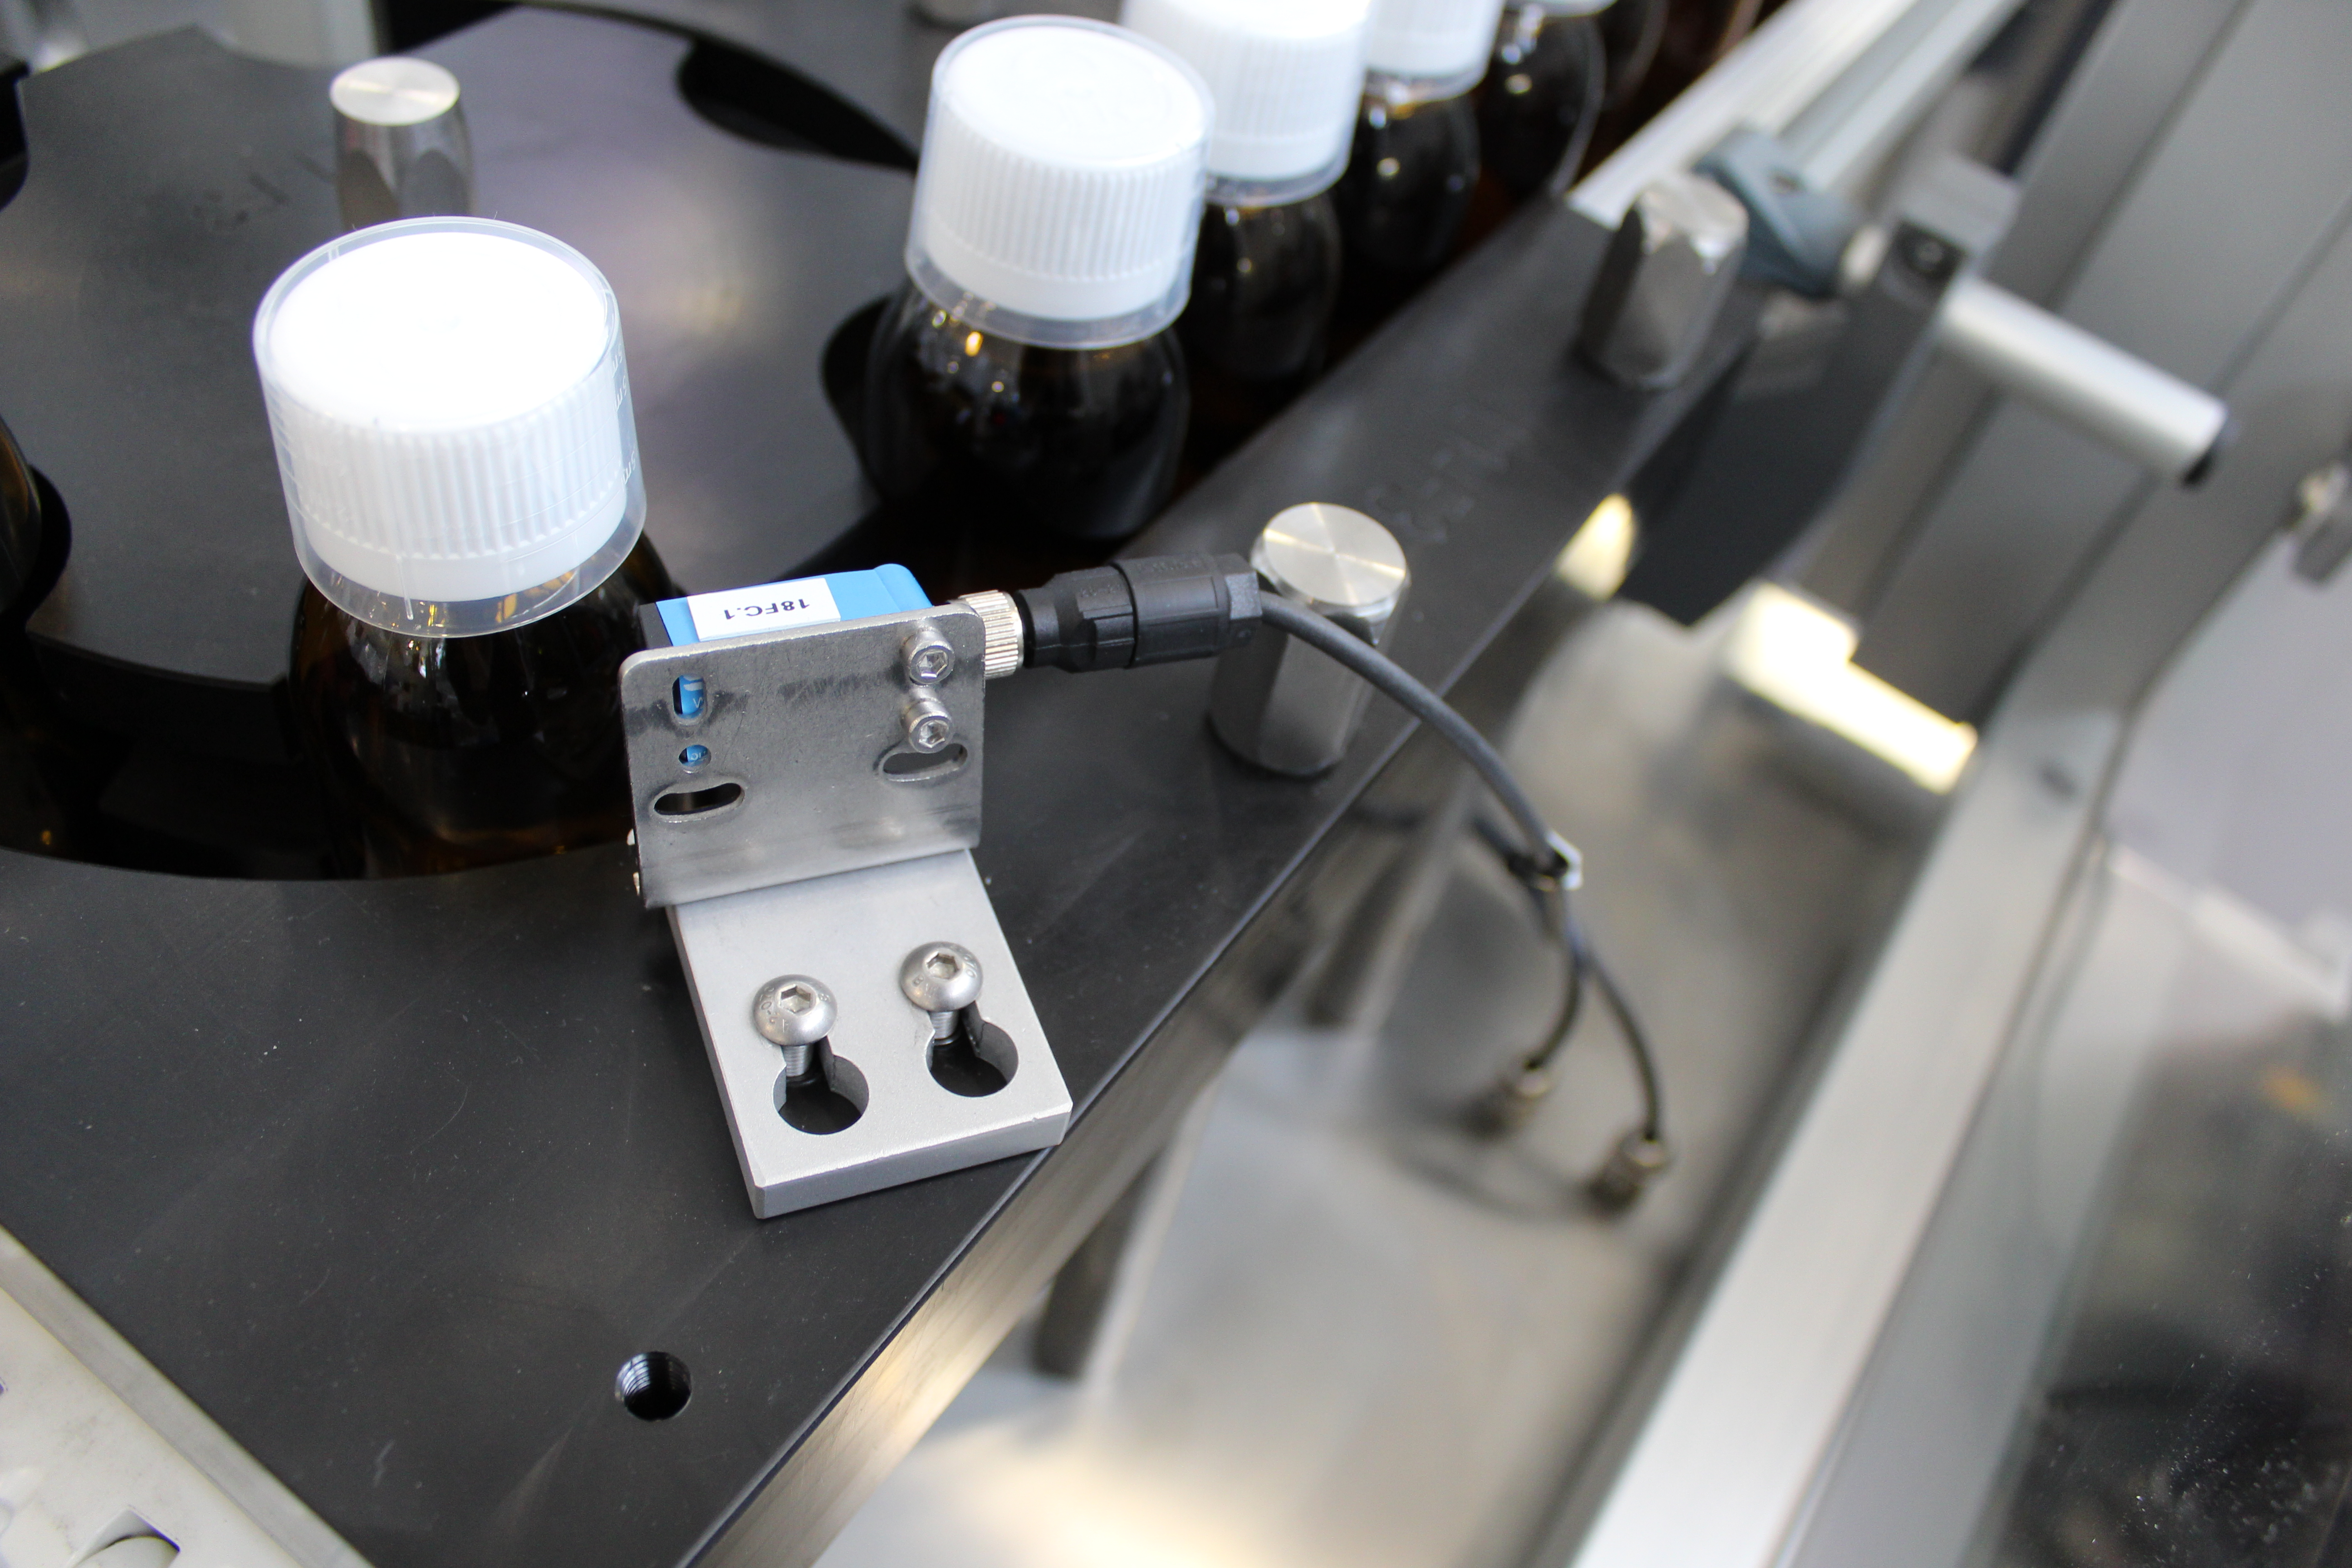
\includegraphics[width=12cm]{Immagini/FLAC1}
	\caption{ Flacone su sensore Ingresso}
	\label{FLAC1}
\end{figure}

Possiamo creare una camma che si attiva a 20 gradi e si disattiva a 40 gradi all'interno della quale rimanere 'in ascolto' del segnale del sensore per definire se il prodotto è presente o meno.

Per le Camme è stata creata una FB che semplifica la loro gestione e mette a disposizione attraverso il suo database una interfaccia. Tale database è strutturato come in figura \ref{CAMME4}.

Ogni Camma ha 4 variabili che ne permettono l'impostazione e la lettura dello stato:
\begin{itemize}
	\item INIZIO (Real): Valore Impostabile da Programma. Sono i Gradi Encoder nel quale vogliamo che la camma risulti attiva
	\item FINE (Real): Valore Impostabile da Programma. Sono i Gradi Encoder nel quale vogliamo che la camma di disattiva
	\item ATTIVA (Bool): Variabile di Sola Lettura. Questa variabile viene settata a TRUE quando i gradi Encoder letti in tempo reale sono compresi tra i valori impostati su INIZIO e FINE
	\item INCLUSA (Bool): Valore Impostabile da Programma. Variabile che permette di Includere o Escludere la Camma dal Programma. Se per qualche motivo l'operatore voglia disabilitare una camma (Per esempio l'operatore macchina non vuole che venga effettuato il Controllo OCR dalla Telecamera basta disablitare la relativa Camma).
\end{itemize}

\begin{figure}[H]
	\centering
	\includegraphics[width=12cm]{Immagini/CAM1}
	\caption{ Interfaccia DB Camme Macchina}
	\label{CAMME4}
\end{figure}


\section{Controllo Mediante Shift Register}
In un macchinario automatico che richiede come specifica il controllo della qualità e l'idoneità dei pezzi prodotti, è necessario naturalmente tenere traccia della posizione di ogni singolo pezzo presente sulla linea per poi determinarne lo stato (presente, buono, scarto). Questa procedura riulterebbe molto semplice se il macchinario fosse programmato a Fasi. Per programmazione a Fasi intendiamo una macchina che processa un solo pezzo alla volta seguendo varie Fasi sequenziali. Questo metodo oltre a rendere la macchina molto più lenta, non sempre adottabile. L'etichettatrice in questione difatti non contiene Fasi bensì è una macchina a ciclo continuo. Questo lo rende molto più veloce ma anche più complesso. Tenere traccia dello stato dei pezzi è un impresa più ardua. Per questo interviene lo Shift-Register.
Lo Shift-Register in questione è una astrazione a più alto livello di quello conosciuto in Elettronica Digitale ma similare nel funzionamento.

Lo Shift-Register viene inteso in questo caso come un blocco di memoria di tipo Byte o Superiore che in uno specifico istante esegue uno shift di N posizioni di tutti i bit verso una specifica direzione.

Consideriamo ad esempio la Word (16 Bit) in figura \ref{sh1}. Il blocco in alto risulta la Word originaria mentre il blocco in basso corrisponde allo shift di tale Word verso sinistra di 6 posizioni (Supponendo di aver Forzato il valore 0 in ingresso)

\begin{figure}[H]
	\centering
	\includegraphics[width=12cm]{Immagini/SH1}
	\caption{ Shift Register Funzionamento}
	\label{sh1}
\end{figure}

Ora non ci resta che creare gli Shift-Register necessari alla macchina. Solitamente se ne crea uno per ogni controllo sulla macchina. Nel nostro caso avremo i seguenti Shift Register:
\begin{itemize}
	\item Shift Presenza Prodotto
	\item Shift Buono Scarto
	\item Shift Controllo Allineamento
	\item Shift Controllo OCR
	\item Shift Controllo PharmaCode
\end{itemize}

I primi tre Shift sono associati alla posizione e stato dei flaconi all'interno della macchina, mentre gli ultimi 2 sono relativi alla etichettatrice ed alla posizione e stato delle etichette.

\begin{figure}[H]
	\centering
	\includegraphics[width=12cm]{Immagini/SH8}
	\caption{ Database contenente o Shift-Register}
	\label{sh8}
\end{figure}


Analizziamo per semplicità solamente il primo relativo alla Presenza Prodotto così da poter effettuare il primo controllo macchina. Bisogna innanzitutto associare virtualmente ad ogni bit dello Shift una posizione sulla macchina \ref{sh2} Si può notare come le posizioni utili per lo Shift-Register principale sono 12 perciò non è sufficiente un Byte (8 bit) ma abbiamo bisogno di una Word (16 bit) per riuscire a gestire tutte le posizioni.

\begin{figure}[H]
	\centering
	\includegraphics[width=12cm]{Immagini/SH2}
	\caption{Shift Register Presenza e Scarto}
	\label{sh2}
\end{figure}

Ora non ci resta che far scorrere lo shift nella stessa direzione del flusso della macchina ogni qualvolta essa si sposta di una posizione Flacone. Il comando ad eseguire lo Shift deve avvenire in un preciso istante del giro della macchina pertanto utilizziamo le nostre Camme Digitali. Associamo dunque al nostro programma le prime due Camme necesarie:

\begin{itemize}
	\item 'Camma di Attivazione SR Presenza Flacone': determina l'istante in cui deve avvenire lo Shift del Registro 'Presenza Prodotto'. Solitamente la sua attivazione è prossima allo Zero Encoder poiché deve essere la prima cosa ad eseguita ad ogni giro macchina prima di qualunque controllo.
	\item 'Camma di Controllo Presenza Flacone': rappresenta l'istante in cui bisogna andare a leggere il segnale della Fotocellula di ingresso per determinare se il Flacone è presente o meno.
\end{itemize}

Mettiamo ora insieme Camme e Shift-Register per creare il nostro primo Controllo Base. Notiamo nella figura \ref{sh3} come il rung venga abilitato soltanto nell'istante in cui la nostra 'CAMMA1'(Camma di Attivazione SR) risulta attiva, a significare che la macchina si trova in una posizione corretta per eseguire tutto ciò che ne segue sul segmento. Ciò che ne risulta è lo Shift di una posizione verso sinistra del registro 'Shift Presenza Prodotto' (tenendo presente che la LSB si trova sulla Destra).


\begin{figure}[H]
	\centering
	\includegraphics[width=12cm]{Immagini/SH3}
	\caption{ Segmento Ciclo Auomatico attivazione SHL}
	\label{sh3}
\end{figure}

Il prossimo segmento \ref{sh4} illustra invece l'istante di verifica presenza prodotto. Ciò che avviene è abbastanza semplice: prima viene verificato se la CAMMA2 (Camma di Controllo Presenza Flacone) risulta attiva e quindi il Flacone si troverebbe in una posizione corretta per il rilevamento del sensore; una volta attiva la Camma2 si va a leggere il valore della fotocellula di presenza prodotto e se essa risulta impegnata da un flacone allora si va a settare sullo 'Shift Presenza Prodotto' il Bit corrispondnte. Il Bit da settare è riferito alle posizioni virtuali assegnate allo shift precedentemente. Il sensore di presenza prodotto che rileva il flacone si trova nella prima posizione macchina al quale abbiamo assegnato il primo Bit dello Shift ovvero il Bit 0. 

Fatto ciò, per ogni giro macchina verrà eseguito lo spostamento dello 'Shift  Presenza Flacone' e subito dopo il controllo Presenza Flacone con relativo aggiornamento del Bit sullo Shift.

\begin{figure}[H]
	\centering
	\includegraphics[width=12cm]{Immagini/SH4}
	\caption{ Segmento Ciclo Auomatico presenza prodotto}
	\label{sh4}
\end{figure}

Avere lo stato di presenza di un flacone all'interno della macchina è indispensabile per evitare che vengano eseguiti controlli inutili o azionare dispositivi ove non necessario. Nel nostro caso risulterebbe molto dannoso al processo se l'etichettatrice applicasse un etichetta li dove non ci fosse un flacone. L'etichetta verrebbe rilasciata sulla stella e potrebbe causare vari problemi. Con lo Shift-Presenza-Flacone questo problema si evita andando a verificare lo stato del Bit prossimo alla pinna di etichettatura prima di inviare il Trigger all'unità di etichettaggio. 

\begin{figure}[H]
	\centering
	\includegraphics[width=12cm]{Immagini/SH5}
	\caption{Trigger etichettatura ciclo automatico}
	\label{sh5}
\end{figure}

Nella figura \ref{sh5} si evince come il Trigger di Etichettatura avviene all'interno nella relativa CAMMA3 e solo se nella posizione 4 dello 'Shift Presenza Flacone' il Bit è settato a True.

Per quanto riguarda gli Shift-Register relativi all'etichettatrice, esse non dipendono dalla posizione della macchina. Questi Shift-Register servono per determinare l'idoneità dell'etichetta sulla base di controlli OCV e PharmaCode.
\\Questi due Shift-Register hanno orientamento opposto a quelli relativi alla macchina ed hanno il primo Bit in corrispondenza dell'ultima etichetta ovvero quella sulla 'pinna' inoltre lo Shift di questi registri avviene ogni qualvolta viene inviato il Trigger al gruppo di etichettaggio e di conseguenza il rullo delle etichette avanza di un passo. 

\begin{figure}[H]
	\centering
	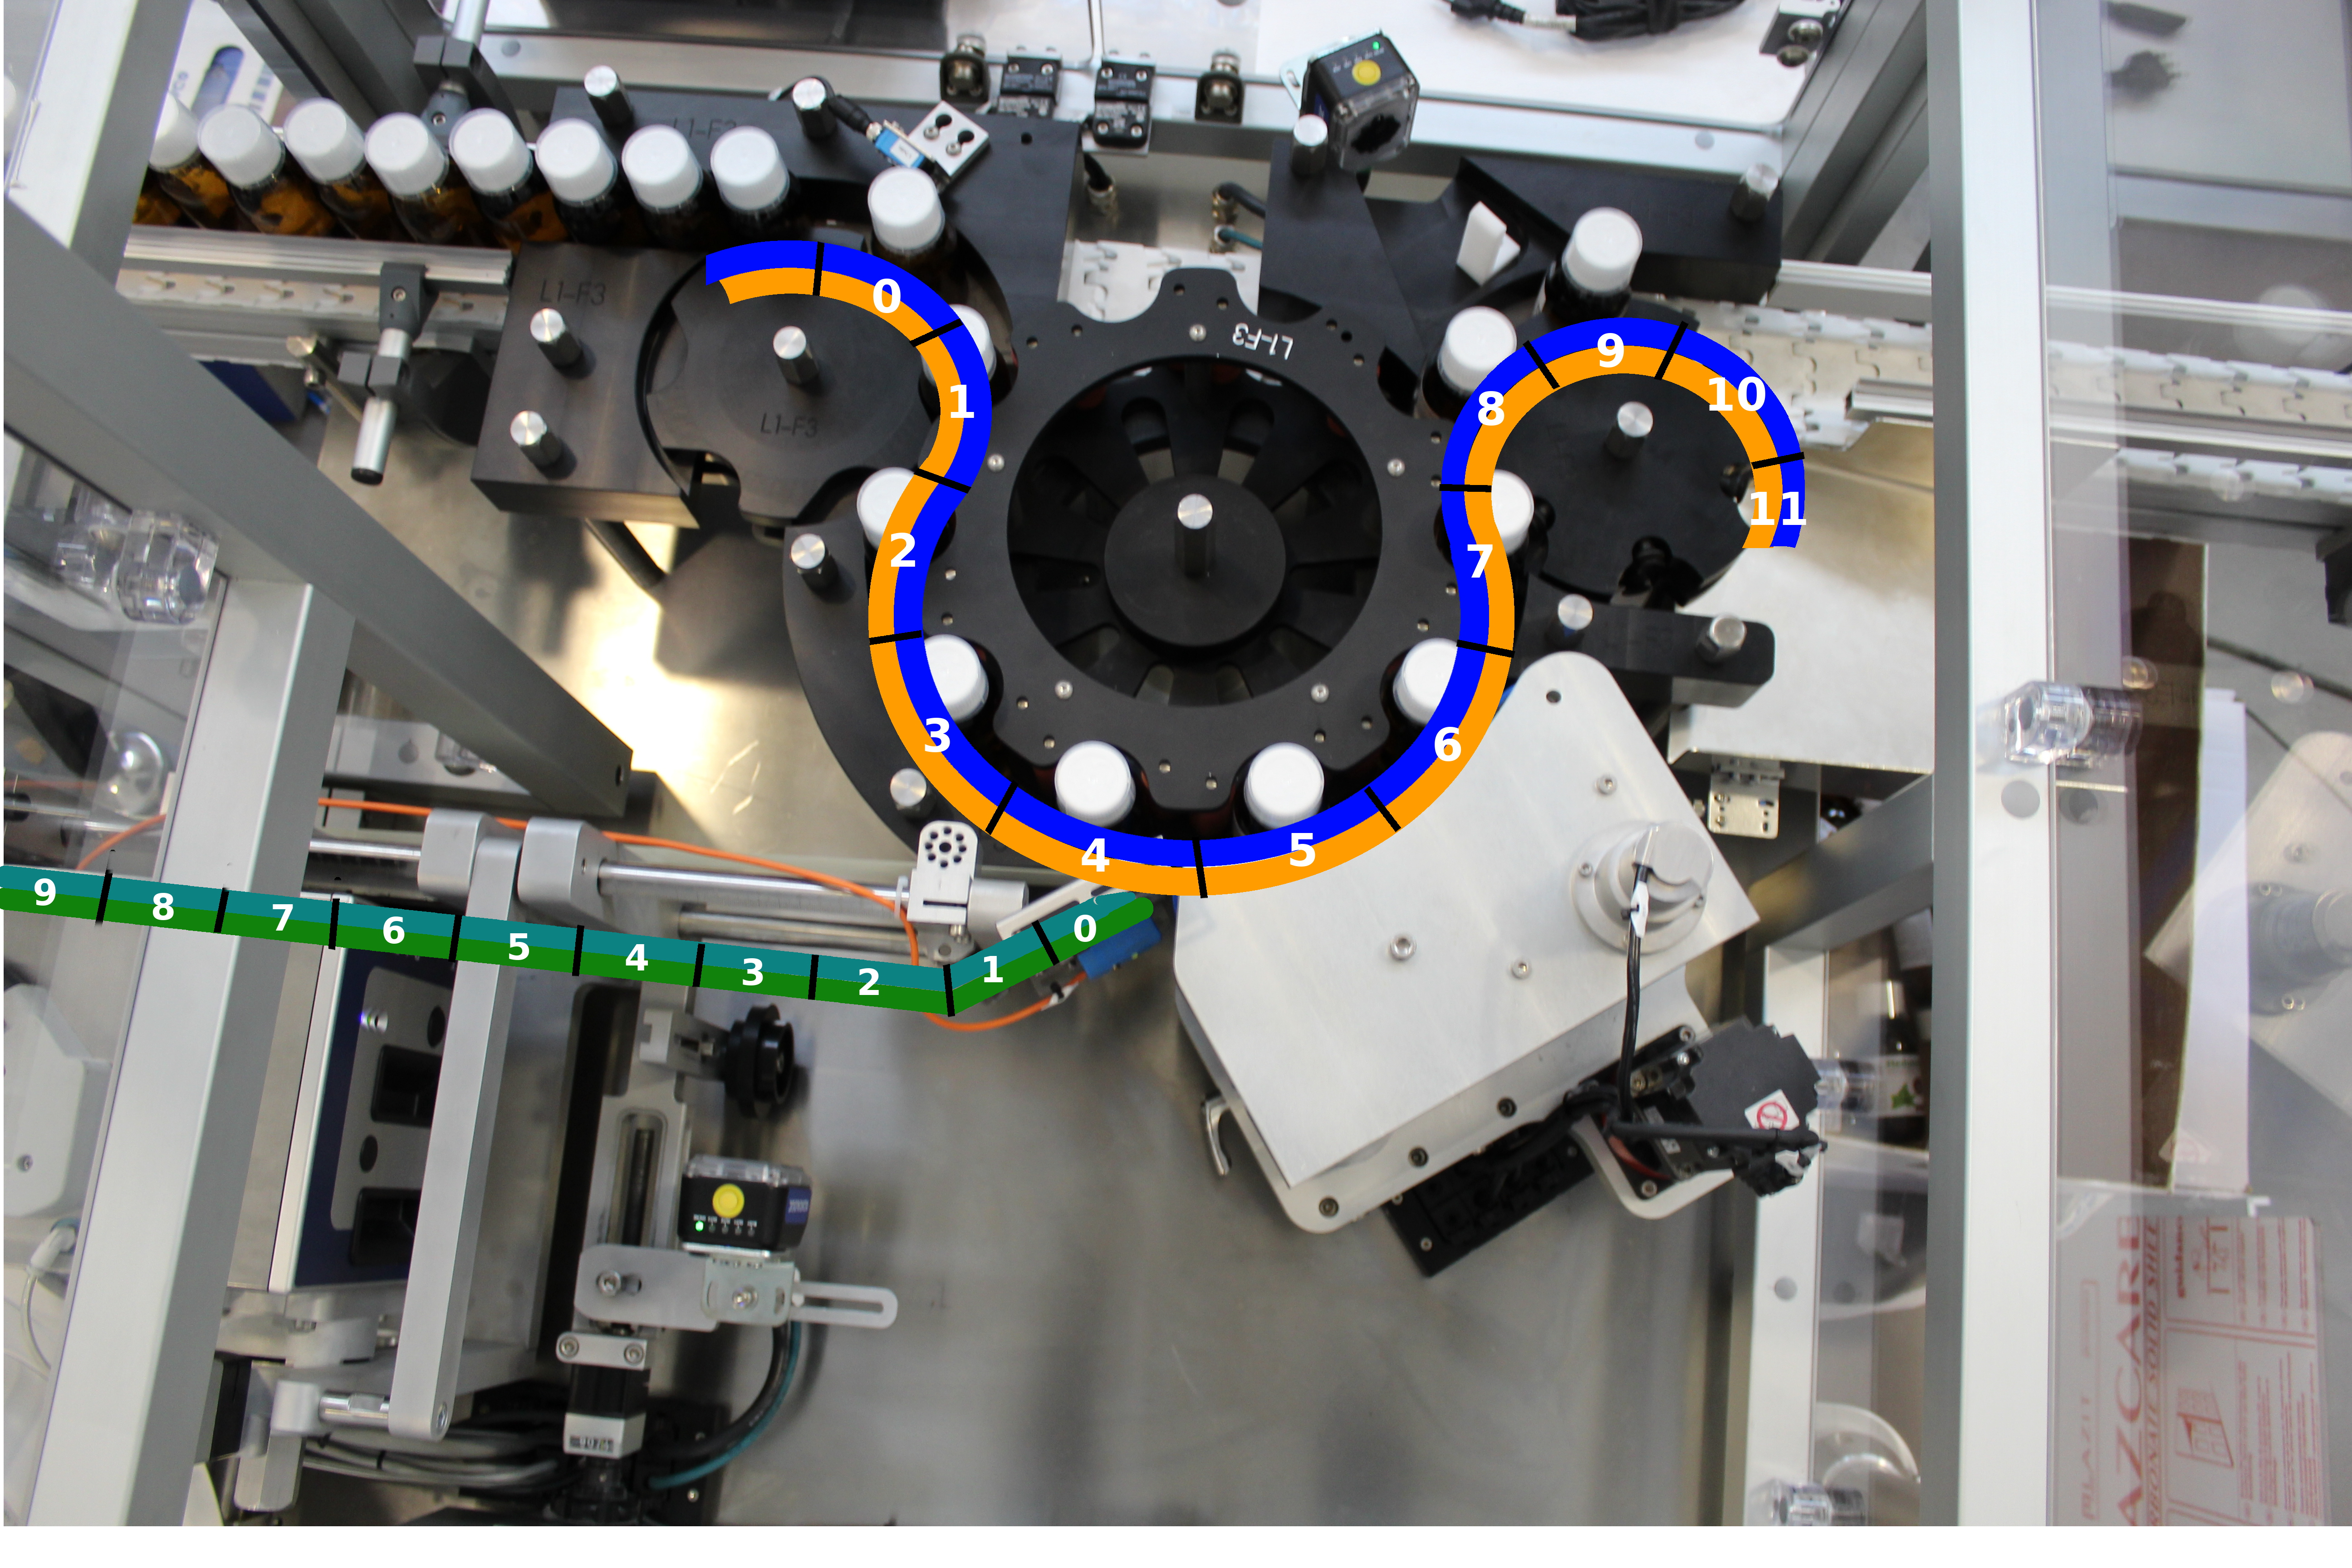
\includegraphics[width=12cm]{Immagini/SH6}
	\caption{Rappresentazione Shift-Register Macchina}
	\label{sh6}
\end{figure}


La gestione di tutto il processo di controllo delle etichette avviene tramite un gioco di Attesa ed Invio di conensi tra Etichettatrice, Stampante e Telecamera. In pratica ciò che succede è riportato di seguito:
\begin{itemize}
	\item Raggiunta la CAMMA3 di 'Trigger Etichetta' viene applicata un etichetta sul flacone
	\item I due 'Shift Controllo OCR' e 'Shift Controllo PharmaCode' vengono shiftati di una posizione verso destra (ricordiamo che lavorano in verso opposto a quelle della macchina)
	\item Non appena viene ricevuto il consenso che l'etichetta è stata espulsa e lo Shift è avanzato, si invia un comando di Trigger alla Stampante ed un Trigger alla Telecamera
	\item La Telecamera elabora il suo programma interno e restituisce sulle sue uscite digitali l'esito del controllo
	\item Se il risultato del controllo è positivo, si setta il Bit dello Shift associato all'etichetta appena controllata a True
	\item Raggiunta nuovamente la CAMMA3 viene applicata l'etichetta sul Flacone e viene Fatto un operazione di AND logico tra i Bit in posizione prossimi alla Pinna degli Shift-Register 'Presenza Prodotto' - 'Controllo Ocr' - 'Controllo PharmaCode' ed il risultato di tale operazione copiata sul Bit dello Shift 'Buono-Scarto'
	\item Sarà infine la terza ed ultima stella del macchinario, in base al valore letto su tale Shift, a decidere se scartare o meno il Flacone. 
\end{itemize}

\begin{figure}[H]
	\centering
	\includegraphics[width=12cm]{Immagini/SH7}
	\caption{Bitwise And Shift-Register}
	\label{sh7}
\end{figure}


\chapter{Protocolli di comunicazione}
Fino a qualche anno fa i diversi fornitori di PLC mantenevano 'segreti' i protocolli di comunicazione e spesso anche i Bus erano 'proprietari'. Anche se sugli impianti continuano a circolare decine o anche centinaia di protocolli diversi, da qualche tempo si avverte la necessità di andare verso protocolli standard. Infatti la maggior parte dei vendor ora utilizzano protocolli conosciuti che in qualche caso sono divenuti standard 'di mercato' o 'di fatto' (come ad esempio ModBus, Profinet, DNP3, DeviceNet, etc).
\\Il PLC durante il suo funzionamento può comunicare con computer, con altri PLC oppure con altri dispositivi come le macchine CNC (i torni e/o le frese a controllo numerico delle aziende). La comunicazione con computer e altri dispositivi avviene tramite tipi di connessione standard: per lo svolgimento della tesi sono stati utilizzati il protocollo Profinet e TCP.
\section{Profinet}
\textit{Profinet} \cite{profinet} è uno standard di automazione aperto che garantisce flessibilità, affidabilità
e performance.
Insieme a Profibus è un leader di mercato nel campo di azionamenti con interfacce digitali. Profinet si basa su IT-Standards, supporta TCP/IP senza limitazioni e consente l'accesso diretto dal livello di gestione aziendale fino al livello di campo. Anche l'integrazione di sistemi e di reti già esistenti non presenta alcun problema con Profinet. Profinet supporta ad esempio l'integrazione di reti Profibus e di altri sistemi di bus di campo, come AS-Interface.  
\subsection{Caratteristiche}
\begin{itemize}
	\item \textit{Safety Integrated}: Safety Integrated soddisfa tutti i requisiti necessari per quanto concerne la sicurezza richiesta per l'uomo, la macchina e l'ambiente. Inoltre, l'utilizzo di Profinet con PROFIsafe consente di creare una rete per la comunicazione standard è orientata alla sicurezza su un solo cavo oppure anche senza fili con Industrial Wireless LAN (IWLAN);
	\item \textit{IT-Standards and Security}: Profinet offre tutte le funzioni per una configurazione e una diagnostica ottimali. Tramite Internet si può accedere a tutti i dati rilevanti da ogni luogo,in tutto il mondo. In questo Profinet soddisfa anche le crescenti esigenze per la sicurezza dei dati e della rete;
	\item \textit{Installazione della rete}: Profinet è basato con coerenza sulla tecnologia Switching a 100 Mbit/s e supporta oltre al cablaggio a stella usuale per Ethernet anche strutture di rete lineari e ad anello. Ciò riduce al minimo l'onere di cablaggio e comporta un elevato grado di flessibilità. La comunicazione senza fili mediante IWLAN offre nuove possibilità di applicazioni nell'industria, persino la funzionalità di servizio e supervisione è possibile senza fili;
	\item \textit{Comunicazione real-time}: Profinet copre l'intera gamma delle applicazioni di automazione offrendo per questo tre tipi di comunicazione di base:
	\\1. Non-Real-Time come la comunicazione TCP/IP e UDP/IP
	\\2. Real-Time (RT) e
	\\3. Isochronous Real-Time (IRT). 
	\\Profinet è quindi adatto anche per applicazioni particolarmente complesse, ad es. nel settore del Motion Control.
	\item \textit{Apparecchiature da campo decentrate}: per il collegamento diretto a Industrial Ethernet di apparecchiature da campo decentrate, \textit{Profibus and Profinet International} ha definito lo standard 'Profinet IO'. Attraverso questo standard le apparecchiature da campo trasmettono ciclicamente i dati all'immagine di processo del relativo controllore. Per l'interazione tra controllori e periferia decentrata, Profinet supporta un modello Provider/Consumer. Il Provider invia al Consumer i propri dati senza richiesta da parte del partner di comunicazione. Quest'ultimo elabora i dati. La correlazione tra Provider e Consumer è definita in fase di progettazione.
	\item \textit{Azionamenti e motion control}: Profinet riduce al minimo l'onere di cablaggio. Che si tratti di comando, operatività, accesso remoto per diagnostica e service, di parametrizzazione e messa in servizio oppure di applicazioni orientate alla sicurezza: tutti
	i compiti vengono eseguiti tramite un cavo che consente di integrare i valori di processo anche in sistemi MES ed ERP. I vantaggi risultanti sono enormi, ad esempio riguardo alla gestione dell'energia e alla manutenzione preventiva. Rende possibile, inoltre, la comunicazione wireless sulla base dei correnti standard WLAN. 
	\item \textit{Intelligenza distribuita}: Profinet offre nuove possibilità nella realizzazione di 	strutture di automazione distribuite: modularizzazione conseguente e comunicazione macchina-macchina semplificata con engineering esteso a tutto l'impianto tramite Component Based Automation.
\end{itemize}


\section{TCP}
Il \textit{Transmission Control Protocol} (TCP) \cite{TCP} è un protocollo di rete a pacchetto di livello di trasporto, appartenente alla suite di protocolli Internet, che si occupa di controllo di trasmissione ovvero rendere affidabile la comunicazione dati in rete tra mittente e destinatario. Il TCP può essere classificato al livello trasporto (OSI level 4) del modello di riferimento OSI, e di solito è usato in combinazione con il protocollo di livello rete (OSI level 3) IP. La corrispondenza con il modello OSI non è perfetta, in quanto il TCP e l'IP nascono prima del suddetto modello. I livelli TCP/IP hanno questa relazione con quelli OSI:
\begin{figure}[H]
	\centering
	\includegraphics[width=12cm]{Immagini/1}
	\caption{ Relazione fra i livelli OSI e TCP/IP.}
\end{figure}
TCP è un protocollo orientato alla connessione e offre funzionalità di controllo di errore sui pacchetti pervenuti grazie al campo checksum contenuto nella sua PDU. Possiede inoltre funzionalità di controllo di flusso tra terminali in comunicazione e controllo della congestione sulla connessione, attraverso il meccanismo della finestra scorrevole. Questo permette di ottimizzare l'utilizzo dei buffer di ricezione/invio sui due end devices (controllo di flusso) e di diminuire il numero di segmenti inviati in caso di congestione della rete.
\\Per poter applicare il modello TCP/IP a tutti i terminali, cioè indipendentemente dal sistema operativo, il sistema di protocollo TCP/IP è stato scomposto in più moduli ciascuno con un compito preciso. Questi moduli svolgono inoltre i compiti gli uni dopo gli altri in un ordine preciso, con un sistema stratificato, ragione per cui si parla di modello a livelli. Il termine livello è usato per evocare il fatto che i dati che transitano sulla rete attraversano più livelli di protocolli. Così, i dati (pacchetti di informazioni) che circolano sulla rete sono trattati successivamente per ogni livello, che aggiunge un elemento d'informazione (detto intestazione) e poi li trasmette al livello successivo. Il modello TCP/IP è molto simile al modello OSI (con 7 livelli) che è stato elaborato dall'organizzazione internazionale degli standard (ISO, organizzazione internazionale di standardizzazione) per standardizzare le comunicazioni tra computer. 
\subsection{Server e client}
I due processi che comunicano attraverso una connessione TCP hanno ruoli diversi:
\\Il processo che avvia una nuova connessione TCP è detto client, invia una richiesta di connessione verso una determinata porta.
Affinché la connessione venga stabilita, su quella porta deve esserci un processo server 'in ascolto', che accetta di stabilire una connessione TCP.
Le porte conosciute e registrate sono quindi utilizzate dai processi server, e sono convenzionalmente associate a particolari servizi, in modo che un client sappia a quale porta connettersi per raggiungere un determinato server.
\\Il processo server, che è in ascolto su una certa porta, rimane bloccato in attesa che un client si colleghi. Il processo client richiede di stabilire una connessione verso un determinato server su una determinata porta. Normalmente la porta sorgente usata dal client viene allocata dinamicamente dal sistema operativo del client. Quando il TCP stabilisce la connessione, a entrambi i processi viene assegnato un socket tramite cui essi possono comunicare tra loro. Tipicamente il processo server effettua una fork, affida al figlio il compito di comunicare con il nuovo client e si rimette in ascolto. Da questo punto in poi, client e server hanno ruoli simmetrici, e utilizzano gli stessi strumenti per comunicare attraverso il socket.
\subsection{Incapsulamento dei dati}
Durante una trasmissione, i dati attraversano alcuni degli strati al livello del terminale emittente. Ad ogni livello, un'informazione viene aggiunta al pacchetto di dati, si tratta di un'intestazione, un insieme di informazioni che garantisce la trasmissione. A livello del terminale ricettore, al momento del passaggio in ogni livello, l'intestazione viene letta, poi cancellata, così, alla ricezione, il messaggio è nel suo stato originale. Ad ogni livello, il pacchetto cambia aspetto, dato che gli si aggiunge un'intestazione, e quindi le denominazioni cambiano seguendo i livelli: 1) Il pacchetto di dati è detto messaggio al livello \textit{Applicazione}; 2) Il messaggio in seguito è incapsulato sotto forma di segmento nel livello \textit{Trasporto}; 3) Il segmento, una volta incapsulato, nel livello \textit{Internet} prende il nome di datagramma; 4) Infine, si parla di frame sul livello \textit{Accesso di rete}.
\subsection{Descizione livelli} 
\subsubsection{Livello Accesso di rete (host to network)}
Il livello Accesso di rete è il primo livello della pila TCP/IP capace di accedere ad una qualsiasi rete fisica, cioè rappresenta i mezzi per realizzare una trasmissione di dati attraverso una rete. Così, il livello Accesso di rete contiene tutte le specifiche riguardo la trasmissione di dati su una rete fisica, che si tratti di rete locale (Token ring, Ethernet, FDDI), di connessione ad una linea telefonica o a qualsiasi tipo di collegamento di rete. Si incarica delle nozioni seguenti: 
\begin{itemize}
	\item invio dei dati sul collegamento; 
	\item coordinamento della trasmissione dei dati (sincronizzazione); 
	\item formato dei dati; 
	\item conversione dei segnali (analogico/digitale); 
	\item controllo degl errori all'arrivo.
\end{itemize}
Fortunatamente tutte queste specifiche sono trasparenti per l'utente, dato che l'insieme di questi compiti è in effetti realizzato dal sistema operativo, come per altro i driver dell'hardware che permettono la connessione alla rete (ad esempio driver della scheda di rete).
\subsubsection{Il livello Internet}
Il livello internet è il livello 'più importante' (sono tutti importanti) dato che è quello che definisce i datagrammi, e che gestisce le nozioni d'indirizzamento IP. Esso permette l'invio dei datagrammi (pacchetti di dati) verso dei terminali remoti nonché la gestione della loro frammentazione e riassemblaggio alla ricezione. 
\subsubsection{Il livello di trasporto}
I protocolli dei livelli precedenti permettevano di inviare delle informazioni da un terminale all'altro. Il livello Trasporto permette a delle applicazioni che girano su terminali remoti di comunicare. Il problema consiste dell'identificare queste applicazioni. In effetti, a seconda del terminale e del suo sistema operativo, l'applicazione potrà essere un programma, un compito, un processo, ecc. Inoltre, la denominazione dell'applicazione può variare da un sistema all'altro, ed è la ragione per cui un sistema di numero è stato realizzato per poter associare un tipo di applicazione ad un tipo di dati; questi identificativi sono detti porte. Il livello Trasporto contiene due protocolli che permettono alle due applicazioni di scambiare dei dati indipendentemente dal tipo di rete scelta (cioè indipendentemente dai livelli inferiori, ecc.). Si tratta dei seguenti protocolli: TCP, un protocollo orientato connessione che assicura il controllo degli errori; UDP, un protocollo senza connessione il cui controllo d'errore è obsoleto. 
\subsubsection{Il livello applicazione}
Il livello Applicazione è quello situato alla sommità dei livelli dei protocolli TCP/IP. Esso contiene le applicazioni di rete che permettono di comunicare grazie ai livelli inferiori. I software di questo livello comunicano quindi grazie ad uno dei due protocolli del livello inferiore (il livello trasporto) cioè TCP o UDP. 
\\Le applicazioni di questo livello sono di differenti tipi, ma la maggior parte sono dei servizi di rete, cioè delle applicazioni fornite all'utente per assicurare l'interfaccia con il sistema operativo. Possiamo classificarli secondo i servizi che offrono: servizi di gestione (trasferimento) di file e di stampa, servizi di connessione alla rete, servizi di connessione remota, le diverse utility di Internet (figura \ref{1}). 
\begin{figure}[H]
	\centering
	\includegraphics[width=12cm]{Immagini/2}
	\label{1}
	\caption{ Relazione fra i livelli e protocolli dell'architettura TCP/IP.}
\end{figure}

\section{Open Platform Communications (OPC)}
OPC \cite{OCP} è lo standard di interoperabilità per lo scambio sicuro e affidabile di dati nello spazio di automazione industriale e in altri settori. È indipendente dalla piattaforma e garantisce il flusso continuo di informazioni tra i dispositivi di più fornitori. La Fondazione OPC è responsabile dello sviluppo e della manutenzione di questo standard.
Lo standard OPC è una serie di specifiche sviluppate da venditori del settore, utenti finali e sviluppatori di software. Queste specifiche definiscono l'interfaccia tra client e server, nonché server e server, compreso l'accesso ai dati in tempo reale, il monitoraggio di allarmi ed eventi, l'accesso ai dati storici e altre applicazioni.
\\Quando lo standard fu rilasciato per la prima volta nel 1996, il suo scopo era quello di astrarre protocolli specifici del PLC (come Modbus, Profibus, ecc.) In un'interfaccia standardizzata che permettesse ai sistemi HMI / SCADA di interfacciarsi con un 'uomo medio' che convertisse generico- OPC leggere / scrivere richieste in richieste specifiche del dispositivo e viceversa. Di conseguenza, è emersa un'intera industria di prodotti artigianali che consente agli utenti finali di implementare sistemi che utilizzano i migliori prodotti interagendo perfettamente tramite OPC.
\\Inizialmente, lo standard OPC era limitato al sistema operativo Windows. Come tale, l'acronimo OPC è stato generato da OLE (object linking and embedding) per Process Control. Queste specifiche, che ora sono conosciute come OPC Classic, hanno goduto di un'adozione diffusa in diversi settori, tra cui produzione, automazione degli edifici, petrolio e gas, energie rinnovabili e servizi pubblici, tra gli altri.
\\Con l'introduzione di architetture orientate ai servizi nei sistemi di produzione sono arrivate nuove sfide nella sicurezza e nella modellazione dei dati. La OPC Foundation ha sviluppato le specifiche OPC UA per soddisfare queste esigenze e, allo stesso tempo, ha fornito un'architettura a piattaforma aperta ricca di funzionalità che era a prova di futuro, scalabile ed estensibile.
\\Oggi l'acronimo OPC sta per Open Platform Communications.
\\Questi sono solo alcuni dei motivi per cui così tanti membri e altre organizzazioni tecnologiche (collaborazioni) si stanno rivolgendo a OPC UA per la loro piattaforma di interoperabilità.
\subsection{Architettura client/server}
OPC si presenta come un'architettura client/server che permette ad un qualsiasi processo (Client) basato su OPC di accedere a qualsiasi sorgente di dati (Server) dotata di interfacce OPC. I fornitori hardware offrono un Server OPC, che permette a qualsiasi applicazione Client di accedere ai dati da esso pubblicati. I server OPC forniscono un metodo per molti pacchetti software diversi (purché si tratti di un client OPC) per accedere ai dati da un dispositivo di controllo del processo, come un PLC o un DCS. Tradizionalmente, ogni volta che un pacchetto richiedeva l'accesso ai dati da un dispositivo, un'interfaccia personalizzata o un driver, doveva essere scritto. Lo scopo di OPC è definire un'interfaccia comune che venga scritta una sola volta e quindi riutilizzata da qualsiasi business, SCADA, HMI o pacchetti software personalizzati.
\\Una volta che un server OPC è stato scritto per un particolare dispositivo, può essere riutilizzato da qualsiasi applicazione in grado di agire come client OPC. I server OPC utilizzano la tecnologia OLE di Microsoft (nota anche come Component Object Model o COM) per comunicare con i client. La tecnologia COM consente di definire uno standard per lo scambio di informazioni in tempo reale tra applicazioni software e hardware di processo.
\\È importante notare che alcune specifiche OPC sono pubblicate, altre sono disponibili solo per i membri della OPC Foundation. Quindi, mentre nessuna azienda 'possiede' OPC e chiunque può sviluppare un server OPC, indipendentemente dal fatto che siano o meno membri della OPC Foundation, i non membri non utilizzeranno necessariamente le specifiche più recenti. Chiunque può integrare i prodotti OPC e non esiste alcun pre-requisito per l'integratore di sistemi di appartenere a qualsiasi organizzazione. Spetta quindi a ciascuna società che richiede prodotti OPC di garantire che i propri prodotti siano certificati e che i loro integratori di sistemi dispongano della formazione necessaria.
In figura \ref{OPC} è possibile osservare le percentuali dei campi di utilizzo di OPC.
\begin{figure}[H]
	\centering
	\includegraphics[width=13cm]{Immagini/OPC}
	\label{opc}
	\caption{Campi di utilizzo OPC.}
\end{figure}
\subsection{Unified Architecture}
Nella tesi è stata usata la versione Unified Architecture: OPC Unified Architecture (UA), pubblicato nel 2008, è un'architettura orientata ai servizi indipendente dalla piattaforma che integra tutte le funzionalità delle singole specifiche OPC Classic in un unico framework estendibile. Questo approccio a più livelli raggiunge gli obiettivi di specifiche di progettazione originali di:
\begin{itemize}
	\item \textit{Equivalenza funzionale}: basandosi sul successo di OPC Classic, OPC UA è stato progettato per migliorare e superare le capacità delle specifiche OPC Classic. OPC UA è funzionalmente equivalente a OPC Classic, ma capace di molto di più (ad esempio trova la disponibilità di OPC Server su PC e / o reti locali, o ancora permette di leggere e scrivere dati/informazioni in base alle autorizzazioni di accesso).
	\item \textit{Indipendenza dalla piattaforma}: da un microcontroller incorporato a un'infrastruttura basata su cloud; OPC UA fornisce l'infrastruttura necessaria per l'interoperabilità in tutta l'azienda, da macchina a macchina, da macchina a impresa e tutto ciò che è intermedio.
	\item \textit{Sicuro}: una delle considerazioni più importanti nella scelta di una tecnologia è infatti proprio la sicurezza. OPC UA è adatto al firewall e risolve i problemi di sicurezza fornendo una suite di controlli mediante crittografia, autenticazione e auditing.
	\item \textit{Estendibile}: possibilità di aggiungere nuove funzionalità senza influire sulle applicazioni esistenti; l'architettura multistrato di OPC UA offre una struttura 'a prova di futuro'. Tecnologie e metodologie innovative come nuovi protocolli di trasporto, algoritmi di sicurezza, standard di codifica o servizi applicativi possono essere incorporati in OPC UA mantenendo la retrocompatibilità per i prodotti esistenti.
	\item \textit{Modellazione completa delle informazioni}: la struttura di modellazione delle informazioni di OPC UA trasforma i dati in informazioni. Con capacità complete orientate agli oggetti, anche le strutture multi-livello più complesse possono essere modellate ed estese. I tipi di dati e le strutture sono definiti nei profili. Ad esempio, le specifiche OPC Classic esistenti sono state modellate in profili UA che possono essere estesi anche da altre organizzazioni (fig \ref{OPC2}).
	\begin{figure}[H]
		\centering
		\includegraphics[width=13cm]{Immagini/OPC2}
		\label{OPC2}
		\caption{Estensione modello.}
	\end{figure}
\end{itemize}

\chapter{Sviluppo Sistema di Visione}
Abbiamo parlato finora di come sviluppare il software PLC che controlla la nostra etichettatrice, come gestire i vari controlli mediante l'utilizzo di camme e di shift Register ma non è stato ancora menzionato come questi controlli vengono realmente effettuati. In questo capitolo andiamo a scoprire cosa accade dietro il 'Trigger Telecamere' continumente citato in precedenza.
Abbiamo già detto che questo specifico Trigger viene inviato ogni volta che l'etichettatrice avanza di un passo. A seguito dell'invio di questo trigger la Telecamera esegue il suo programma di Visione, ne elabora il risultato ed in caso di risultato positivo attiva la sua uscita digitale inviando un segnale al PLC. Questo segnale rappresenta l'idoneità dell'etichetta appena controllata.
\\Nel presente capitolo si parlerà dello sviluppo del sistema di visione. I Sistemi di visione si realizzano utilizzando in modo opportuno una serie di dispositivi elettro-ottici e meccanici per svolgere generalmente le seguenti fasi:
\begin{itemize}
	\item Generazione dell'informazione, che consiste nel caratterizzare fisicamente in modo visivo ciò che interessa il controllo in oggetto
	\item Acquisizione delle immagini, cioè trasferire l'informazione grafica in una serie di punti digitalizzati sul computer
	\item Elaborazione delle immagini che è la fase di estrazione delle caratteristiche interessanti il controllo e la loro valutazione quantitativa
	\item Interpretazione automatica dei risultati, che attraverso una serie di criteri di scelta e di controllo, devono arrivare ad un risultato univoco ed automatico.
\end{itemize} 

In questo modo è possibile misurare in modo oggettivo le caratteristiche dei prodotti e le prestazioni della linea di produzione, così come valutare rapidamente l'effetto che altre variazioni esterne hanno sulle caratteristiche del prodotto.
\\Nel progetto della LabelTech abbiamo utilizzato un sistema di visione della Datalogic per eseguire i controlli di qualità ed idoneità del prodotto elaborato dalla macchina.
\\Nelle prossime sezioni verrà descritto nel dettaglio lo sviluppo di questo specifico sistema di visione.

\subsection{Datalogic Impact Sofwtare Suite}
Dataglogic mette a disposizione degli sviluppatori una Suite di applicazioni proprietarie per la reazione dei programmi di visione. I tool principali di questa Suite sono:

\begin{itemize}
	\item \textit{VPM}: è il programma principale per poter configurare la camera. Permette, prima
	di tutto, di settare i parametri principali (apertura shutter, trigger, illuminatori,
	calibrazione ecc) per un corretto funzionamento a seconda delle condizioni operative
	dell'utente. In secondo luogo, è necessario per poter creare il task di ispezione
	desiderato. Creando un file di ispezione si avrà la possibilità di utilizzare i diversi
	tool presenti. I tool vanno dal semplice Blob detection al più complicato Pin Point
	Tool. Combinando tutti questi tool l'utente potrà individuare in modo univoco un
	particolare oggetto che verrà acquisito dalla camera e volendo, fornire le coordinate
	di esso ad un altro dispositivo. Il file di ispezione che si viene a creare viene
	chiamato vision program (.vp).
	\item \textit{CPM}: questo programma invece serve per creare l'interfaccia utente in maniera da essere utilizzata in real time mentre all'interno della camera il file di ispezione, precedentemente configurato, esegue le sue operazioni. Permette quindi, ad esempio,
	di vedere a video i risultati dell'ispezione e di modificare alcune configurazioni in
	maniera rapida. Infatti rispetto ai complessi linguaggi di programmazione, CPM
	offre la massima flessibilità e consente di creare pannelli di controllo in tempi decisamente
	inferiori a quelli normalmente richiesti. Rappresenta la vera e propria
	HMI (Human Machine Interface) della camera.
	\item \textit{IMPACT SDK}:quest ultimo non è un vero e proprio software. È una libreria scritta in C\# che integrata ad un progetto di Visual Studio permette di utilizzare delle classi e metodi per interagire con la camera. Attraverso queste APIs (Application Program Interface) l'utente può sviluppare la proprio HMI perfettamente. Quindi il CPM e la libreria SDK vengono utilizzate per lo
	stesso fine anche se quest'ultima richiede una maggiore abilità di programmazione (conoscenza del C \#) ma permette una maggiore flessibilità. Tramite i metodi è possibile infatti poter richiamare qualunque tool della camera già utilizzato nel VPM. Le principali APIs di cui si pu`o usufruire sono:
	– Connessione/disconnessione ad un Vision Device.
	– Caricare programmi di ispezione.
	– Caricare o scaricare immagini dal/verso il pc.
	– Ricavare dati dall'immagine.
	– Calibrare la camera.
	– Scattare fotografie.
\end{itemize}

\subsection{Datalogic VPM}
Il Vision Program Manager di Datalogic è il tool per eccellenza che permette di sviluppare il programma e la logica di controllo delle immagini catturate dalla telecamera. I tool che Datlogic mette a disposizione sono suddivise in Macro-Categorie:
\begin{itemize}
\item Manipolazione Immagine: Questi tool permettono la anipolazione dell'immagine rilevata dalla telecamere mediante l'applicazione di specifici filtri e distorsioni. Questi tool servono a preparare l'immagine per la vera e propria elaborazione. Per esempio spesso si potrebbe voler eseguire l'elaborazione su una immagine in Bianco e Nero con elevato Contrasto pertanto filtrare l'immagine per renderla più idonea ai Task che verranno eseguiti. 
	\item Localizzazione : Sono quei tool necessari a Localizzare parti dell'immagine di interesse. Uno Spigolo, un cerchio, o semplicemente una feature dell'immagine sulla quale era stato effettuato un Train mediante il tool 'PinPointPatternFinder'. La localizzazione di feature serve spesso come sistema di riferimento per controlli successivi. Immaginiamo di voler verificare tutte le monete di un certo tipo; non possiamo semplicemente utilizzare un tool di Ispezione che confronti l'immagine con un altra sulla quale era stato fatto il Train. Questo perchè la moneta potrebbe non trovarsi sempre nella stessa posizione e pertanto un lieve spostamento della moneta risulterebbe in un test fallito.
	
	\begin{figure}[H]
		\centering
		\includegraphics[width=13cm]{Immagini/VIS1}
		\label{vis1}
		\caption{Immagini di Monete catturate nella medesima applicazione}
	\end{figure}

	Per ovviare a questo tipo di problema molto solito, si usa prima un Locatore che per rilevare un oggetto più generico e successivamente sul riferimento assoluto di quell'oggetto si possono eseguire elaborazioni con tool più specifici. Nell'esempio in questione conviene prima localizzare un elemento di forma circolare; avendo a tal punto un riferimento alla sua origine, possiamo eseguire il controllo limitandoci a solo ciò che si trova al suo interno utilizzando la localizzazione di un Trained Model (ovvero il confronto di una feature con quella di un campione salvato). Il salvataggio del campione viene chiama appunto 'Train' e deve essere rieseguito ogni volta che viene cambiato il modello di riferimento che si desidera ricercare/confrontare
	
		\begin{figure}[H]
		\centering
		\includegraphics[width=13cm]{Immagini/VIS3}
		\label{vis3}
		\caption{Locatore di un trained Model (ROI regione circolare gialla)}
	\end{figure}
	
		\begin{figure}[H]
		\centering
		\includegraphics[width=13cm]{Immagini/VIS2}
		\label{vis2}
		\caption{Locatore di trained Model. Notare il 'Tool Origin' riferito al centro del Locatore Circolare }
	\end{figure}


	
	\item Ispezione: Sono tool che servono appunto per l'ispezione di determinati feature quali Misurazioni, Rilevamento di Difetti, Letture OCR e Data Matrix. Quasi tutti i tool di Ispezione e Localizzazione richiedono che si specifichino delle cosiddette ROI (Region of Interest). Nel caso dei tool di localizzazione e ispezione si richiede sia specificata l'area di ricerca dei cosidetti Feature ed in caso di Localizzazione di Trained Features viene richiesta anche l'area della regione ove eseguire il Train del Modello. 
	
		\begin{figure}[H]
		\centering
		\includegraphics[width=13cm]{Immagini/VIS5}
		\label{vis5}
		\caption{Region of Interest per un controllo OCR (Area di Tratteggio Arancione)}
	\end{figure}
	
	
	\item Logici: I tool logici invece servono per elaborare manualmente i Dati o i risultati ottenuti dai controlli precedenti. Mediante questi si possono controllare per esempio le uscite Digitali e Profinet della telecamera. Si possono inoltre creare Branch, Ciclo, Break, Switch Case ed in essi utilizzare operatori logici quali AND-OR (Supponiamo di volere uscita telecamera positiva solamente se 2 controlli sono soddisfatti). Oltre a tali costrutti ed ai più semplici operatori Logici esistono anche tool che permettono di scrivere interi script in linguaggio BASIC lasciando estrema liberta allo sviluppatore
	
			\begin{figure}[H]
		\centering
		\includegraphics[width=13cm]{Immagini/VIS4}
		\label{vis4}
		\caption{Controllo dell'uscita discreta della telecamera}
	\end{figure}

\end{itemize}

AL termine dello sviluppo del programma di visione essa potrà essere salvata all'interno della telecamera così che venga avviato automaticamente all'accensione e della messa online della stessa. Su una telecamera possono essere salvati più di un programma di visione e la commutazione tra i vari programmi può avvenire mediante speifici comandi Profinet, via TCP ed altri protocolli compatibili oppure creando dei particolari task scritti in linguaggio BASIC che ricevendo segnali sugli ingressi digitali si occupano di elaborare tale richiesta.

\subsection{Datalogic CPM}

Il Datalogic CPM (Control Panel Manager) consente di creare panelli operatore con il quale l'utente utilizzatore del nostro software può interagire. Questo serve sia per evitare che l'utente possa modificare la logica funzionale del programma di visione, sia per dargli un interfaccia restrittiva di solo quello che sarà di sua competenza. Il CPM permette di creare l'interfaccia operatore tramite un software grafico. Mette a disposizione oggetti grafici quali Text-Box, Botton, I/O Display Box ed altri oggetti quali finestre ove visualizzare l'immagine catturata dalla telecamera e modificare le ROI e SEARCH AREA dei vari controlli.

			\begin{figure}[H]
	\centering
	\includegraphics[width=13cm]{Immagini/VIS6}
	\label{vis6}
	\caption{Esempio di Applicazione CPM}
\end{figure}

Concluso lo sviluppo dell'applicazione CPM per eseguirlo basta creare uno script in Visual Basic o un semplice batch script di windows per eseguire il CPM Runtime passandogli come parametro il file di progetto CPM appena creato

\subsection{Programma di Visione LabelTech}
Andiamo ad Aanalizzare ora il programma di visione sviluppato per la nostra Labeltech. Prendiamo in considerazione soltanto la telecamera di controllo etichette e lo sviluppo del suo programma. Lo scopo è quello di verificare che il Pharmacode (Codice a barre specifico nel Pharmaceutico) ed i dati stampati dalla Stampante Videojet siano corretti e non contengano errori di stampa. 

\begin{figure}[H]
	\centering
	\includegraphics[width=13cm]{Immagini/VIS7}
	\label{vis7}
	\caption{Immagine Dell'etichetta catturata da Telecamera}
\end{figure}

Vediamo nel dettaglio il programma di visione sviluppato analizzando uno alla volta i vari controlli che dovranno essere fatti sull'etichetta:

\begin{itemize}
	\item \textit{Controllo Pharmacode Data Matrix}: Il primo controllo ad essere eseguito è la ricerca e verifica della correttezza del PharmaCode. Questa verifica deve controllare sia la correttezza in termini di legibilità ed integrità del Pharmacode ma anche la correttezza del codice stesso. Il valore del codice letto infatti deve corrispondere al valore Pharmacode identificativo del Lotto in produzione.
	

	
	\begin{figure}[H]
		\centering
		\includegraphics[width=13cm]{Immagini/VIS8}
		\caption{Controllo PharmaCode}
		\label{vis8}
	\end{figure}

	Come si può vedere nella figura \ref{vis8} esiste uno specifico tool per la lettura di codici a barre sia 2D che 3D. Questo tool necessita semplicemente che gli sia specificata uno ROI nella quale andare a ricercare il codice. Penserà esso a ritrovare un codice valido in quell'area e determinarne il valore. Il Pass-Fail di questo tool dipende dal fatto che venga rilevato o meno un codice a barre nell'area della ROI e che il valore di tale codice corrisponda ad un valore impostato o rilevato precedentemente da Training. 
	
	\item \textit{Controllo OCR Codice Lotto}: Il secondo controllo si occupa di determinare la corretta stampa del codice lotto da parte della stampante ed anche della verifica che tale codice corrisponda effettivamente al valore Codice Lotto in produzione. Il controllo OCR nella visione è uno dei controlli che richiedono maggiore tempo di calcolo pertanto impostare un ROI di ricerca troppo ampia potrebbe compromettere notevolmente le prestazioni. Inoltre le stampe effettuate dalla stampante potrebbero risultare leggermente spostate da un etichetta all'altra per questo motivo come spiegato precedentemente è preferibile in questi casi utilizzare un locatore.
	Come locatore per questo specifico caso abbiamo deciso di utilizzare l'inizio della stampa stessa. 
	
		\begin{figure}[H]
		\centering
		\includegraphics[width=13cm]{Immagini/VIS9}
		\caption{Locatore Per Controllo OCR}
		\label{vis9}
	\end{figure}

In questo modo abbiamo potuto ridurre al minimo l'area della ricerca del codice OCR poiché tale ROI rimarrà sempre agganciato al punto relativo al locatore.
Sulla base della posizione del locatore, mediante il Tool di rilevamento OCR determiniamo la ROI di ricerca e rilevamento caratteri. Ogni volta che cambiano i caratteri da ricercare bisognerà effettuare un nuovo train dei caratteri. Il train si effettua specificando l'area da leggere e specificando in una textbox i caratteri che si stanno leggendo. Il software della datalogic autoapprenderà il nuovo codice salvando le immagini dei singoli caratteri catturati in una libreria interna. Tale libreria verrà utilizzata come campione di confronto per rendere più veloce ed efficiente le future analisi. 

		\begin{figure}[H]
	\centering
	\includegraphics[width=13cm]{Immagini/VIS10}
	\caption{Controllo OCR Codice Lotto}
	\label{vis10}
\end{figure}

Il Pass-Fail di questo tool verrà deciso anch'esso dall'idoneità e qualità dei caratteri stampati e dalla verifica con una stringa di riferimento alla quale deve corrispondere. Tutte le impostazioni dalla grandezza e posizione delle ROI, alla procedura di Train e l'impostazione della stringa di confronto, potranno essere gestite all'interno del CPM che verrà sviluppato per l'operatore della macchina. 
	
	
	\item \textit{Controllo OCR Codice Scadenza Lotto}: Il terzo ed ultimo controllo di questa telecamera si occupa di determinare la corretta stampa della scadenza e della verifica che essa corrisponda al reale valore di Scadenza del Lotto in produzione. La procedura per eseguire questo controllo è la medesima applicata per il controllo del Codice Lotto tantè che utilizzano il medesimo Locatore poiché si presuppone che la stampa dei valori da parte stampante sia sempre e comunque allineata e se dovesse risultare leggermente spostata l'una lo risulterebbe anche l'altra. 
	
	\begin{figure}[H]
		\centering
		\includegraphics[width=13cm]{Immagini/VIS11}
		\caption{Controllo OCR Scadenza Lotto}
		\label{vis11}
	\end{figure}
	
	Pertanto il Pass-Fail di questo tool anche dipenderà dall'idoneità e qualità della stampa e dalla verifica del valore rilevato dall'OCR con uno di riferimento.

\end{itemize}

Una volta configurati i vari Controlli che al termine di ogni trigger elaboreranno i relativi risultati, dobbiamo definire le logiche generali di Pass-Fail il quale risultato dovrà essere inviato al PLC.
Per fare ciò Datalogic ci mette a disposizione dei tool molto pratici:

\begin{itemize}
	\item \textit{Pass-Fail Branch}: Si tratta di un costrutto di Branch (If-Else) che permette di creare una condizione di Pass o Fail basata sul risultato di uno o più controlli.
	
			\begin{figure}[H]
		\centering
		\includegraphics[width=13cm]{Immagini/VIS12}
		\caption{Pass-Fail Branch}
		\label{vis12}
			\end{figure}
		
		Nella figura \ref{vis11} possiamo vederne il funzionamento. Una volta importato il tool, essa ci mette a disposizione 2 Branch una di PASS ed una di FAIL. Per configurare questo tool è sufficiente definire quale sia la condizione di ingresso nel segmento di PASS. Per definire tale condizione, viene messo a disposizione un box contenente tutte le uscite dei risultati dei tool utilizzati nel programma di visione. Basta a questo punto spuntare i tool che devono essere soddisfatti affinchè sia 'attivato' il segmento di PASS.
		
		\begin{figure}[H]
			\centering
			\includegraphics[width=13cm]{Immagini/VIS13}
			\caption{Discrete Output}
			\label{vis13}
		\end{figure}
	
		Ora non resta che inviare tale risultato al PLC. Nel segmento di Pass perciò utilizziamo il tool 'Discete Output' che ci da un interfaccia per poter scrivere sulle uscite digitali. Mediante questo tool configuriamo l'uscita digitale numero 1 come un impulso digitale. In questo modo, ogni volta che il programma entrerà in quello specifico segmento di PASS, verrà inviato un comando al PLC a comunicare che il controllo ha avuto un esito positivo.
		
		 
\end{itemize}

\subsection{Control Panel Manager LabelTech}
Concluso lo sviluppo del VP (Vision Program) è necessario creare un interfaccia utente che consenta all'operatore di visualizzare in tempo reale l'andamento del controllo, verificare e modificare eventuali ROI dei var controlli, definire i valori di riferimento per le verifiche OCR e PharmaCode e creare diverse configurazioni di questi valori per i diversi formati di prodotti che dovranno essere analizzati. Ogni formato di etichetta diversa infatti avrà una propria confugrazione del Programma di Visione che potrà essere salvato modificato e caricato sulla telecamera in caso di un cambio formato. Di seguito alcuni Screen Shot del CPM sviluppato.

\begin{figure}[H]
	\centering
	\includegraphics[width=13cm]{Immagini/VIS14}
	\caption{Interfaccia Operatore Controllo PharmaCode}
	\label{vis14}
\end{figure}

Nella figura \ref{vis14} è rappresentata l'interfaccia CPM per controllo Parmacode: essa mette a disposizione semplicemente un pulsante di Train del Pharmacode da verificare e cattura automaticamente il valore che verrà utilizzato come campione di riferimento per le successive verifiche. È anche possibile spostare l'area di ricerca ROI.


\begin{figure}[H]
	\centering
	\includegraphics[width=13cm]{Immagini/VIS15}
	\caption{Interfaccia Impostazione Locatore OCR}
	\label{vis15}
\end{figure}

Nella figura \ref{vis15} è rappresentata l'interfaccia operatore per l'impostazione del Locatore OCR. Essa permette all'operatore di definire la feature da utilizzare come Locatore di posizionamento facendo il Training di una determinata feature dell'immagine e impostando poi un area ove effetuarne la ricerca. Sul CPM è stato previsto inoltre uno slider per impostare la 'Percentuale di accuratezza minima' affinchè il controllo risulti idoneo. Naturalmente al momento del train l'immagine rilevata avrà una accuratezza del 100\% con il campione appena catturato.

\begin{figure}[H]
	\centering
	\includegraphics[width=13cm]{Immagini/VIS16}
	\caption{Interfaccia Controllo OCR Scadenza Lotto}
	\label{vis16}
\end{figure}

Nella figura \ref{vis14} è rappresentata l'interfaccia CPM per controllo OCR del Codice Lotto. Questa interfaccia è leggermente più complessa rispetto alle altre poiché necessita della configurazione di diversi parametri. Tra questi parametri vi sono:
\begin{itemize}
	\item Range di spaziatura minima tra le lettere da rilevare
	\item Range di spaziatura massima tra le lettere da rilevare
	\item Stringa di Train nel quale inserire il reale valore del testo da rilevare in modo da creare i campioni di confronto nella libreria interna
	\item Stringa da verificare nel quale l'operatore definisce la stringa con il quale confrontare il testo rilevato dalla telecamera. 
\end{itemize}

\chapter{HMI/SCADA}
Un HMI, o interfaccia uomo-macchina, è un dispositivo o un software che permette al suo utilizzatore di comunicare con un macchinario o un impianto di produzione. Come? Traducendo una quantità immensa di dati complessi in informazioni accessibili all'uomo. In questo modo l'operatore ha a sua disposizione tutti gli strumenti necessari per controllare il processo di produzione.
Contestualizzando questa definizione nel mondo dell'Automazione Industriale, risulta dunque evidente che più intuitivo e user-friendly è l'HMI, più efficiente e redditizio risulta il lavoro.
\\Sostanzialmente un dispositivo HMI rende possibile la visualizzazione e il controllo delle applicazioni. Sfruttando risorse come I/O, SoftPlc CoDeSys o Ethercat e sistemi operativi (ancora meglio se embedded), permette di comunicare con qualsiasi sistema aziendale.

Un sistema di supervisione viene generalmente impiegato per controllare una realtà complessa, dove l'acquisizione di una grande quantità di dati in tempo reale, la sua elaborazione, interpretazione e presentazione sono essenziali per il funzionamento di impianto, dal momento che le decisioni riguardanti la conduzione vengono prese proprio in base a tali dati, la loro raccolta non può essere effettuata manualmente. Sostanzialmente i sistemi di supervisione si dividono in due categorie che sono le seguenti:
\\a) Sistemi HMI (Human Machine Interface)
\\b) Sistemi SCADA (Supervisory Control And Data Acquisition)
\\I sistemi HMI sono generalmente impiegati a bordo macchina,  cioe nelle immediate vicinanze della macchina che si vuole controllare. I sistemi SCADA sono ache essi fondamentalmente degli HMI e per molti aspetti più evoluti rispetto agli HMI standard.La differenza più grande rispetto agli HMI consiste ne fatto che i sistemi SCADA possono memorizzare i valori di processo rilevati anche per lunghi periodi di tempo. Questi sistemi hanno una sorta di database per la memorizzazione di tali dati. Tutti i sistemi SCADA vengono integrati o appoggiati su sistemi di database. Solitamente i database sono software commerciali sviluppati da terzi, come esempio Microsoft SQL, Oracle,DB2 ect. Oltre ai DB commerciali vengono impiegati anche DB open source come PostgreSQL, MYSQL ect. Un altra differenza tra SCADA e gli HMI standard risiede nel fatto che sistemi SCADA non vengono impiegati a bordo macchina. Questi sistemi effettuano un controllo da postazioni remote via rete, per questo motivi vengono anche chiamati sistemi di supervisione e raccolta dati. In seguito verranno illustrati i componenti che costituiscono un sistema di supervisione come avviene la comunicazione tra essi,  il processo di sviluppo e quali requisiti devono essere soddisfatti. 


\subsection{Tipologie di HMI}
In un sistema di supervisione è importante il modo in cui avviene l'interazione uomo-macchina. I dispositivi HMI stanno assumendo un ruolo sempre più decisivo nelle applicazioni di automazione sia industriale che civile, infatti la possibilità di visualizzare in tempo reale messaggi diagnostici,  allarmi o istruzioni per l'operatore e al contempo modificare i parametri operativi in modo semplice e diretto è diventata un'esigenza essenziale nella maggior parte delle applicazioni. Nel caso dell'attivita di controllo di un impianto di produzione l'utente dovrà essere in grado di visualizzare lo stato degli elementi che compongono questo impianto ad esempio sonde di temperatura, di umidita, posizionamenti di parti mobili del impianto ecc, inoltre l'utente dovra essere in grado di impartire comandi al impianto ed effettuare regolazioni. L'interazione uomo-macchina avviene attraverso la riproduzione di tutti i pannelli di controllo dei regolatori di temperatura, allarmi, ed altri attuatori. È il supervisore a farsi carico del controllo del regolare funzionamento degli apparati, della segnalazione di anomalie e dell'esecuzione o suggerimento di azioni correttive. Si avverte sempre più l'esigenza di visualizzare, controllare e interagire con i sistemi da postazioni remote. La tendenza del mercato HMI riflette le linee di evoluzione introdotte dal fenomeno della convergenza digitale: le applicazioni e i dispositivi si sono fatti sempre più flessibili e potenti, consentendo remotizzazione, multicanalità, mobilita, personalizzazione e adattamento a diversi tipologie di rete, mentre le interfacce utente e le architetture applicative si sono uniformante ad alcuni tra i principali standard tecnologici emersi sul mercato, architetture basate su indirizzamento IP,ISO/OSI,architetture a 3 livelli ecc. Sostanzialmente oggi sul mercato esistono diverse tipologie di HMI, che vanno da semplici display con linee di testo nei quali si possono visualizzare informazioni testuali, a display grafici nei quali assieme al testo sono presenti anche informazione grafiche. Alcuni di questi sistemi integrano le funzionalità dei PC desktop e vengono chiamati panel PC, sostanzialmente è un sistema di calcolo integrato in un display grafico dota to di sistema operativo, generalmente Microsoft Windows, Windows CE.
Questi sistemi possiedono tutte le funzionalità sia grafiche che di comunicazione dei PC. Tuttavia una limitazione di questi dispositivi è data dalla dimensione dello schermo che nei modelli più economici è ridotta di conseguenza si ha una limitazione nelle applicazioni grafiche.

\textcolor{red}foto dei vari tipi di HMI testuale shermo Siemens e HMI MICROSOFT

\subsection{Progettazione di un' Interfaccia}
Con l'avvento dei servizi web come punti centrali per la condivisione di informazioni e di dati, gli utenti hanno sentito la necessita di accedere e gestire le informazioni di lavoro, personali, da qualsiasi luogo in qualsiasi momento e con qualsiasi dispositivo (computer, palmare, cellulare, televisione ecc), di conseguenza la progettazione di applicazioni per dispositivi si è considerevolmente evoluta. Quando si progetta l'interfaccia di una applicazione è necessario considerare molti elementi relativi al dispositivo di destinazione, come la risoluzione, la dimensione e gli angoli di visualizzazione dello schermo, i colori, i caratteri, in quanto le applicazioni vengono visualizzate diversamente a seconda del dispositivo. L'obiettivo consiste nello sviluppare applicazioni più rapide, produttive semplici ed esteticamente gradevoli e di facile comprensione ed utilizzo da parte del utente finale. I principali vincoli di progettazione di una interfaccia utente che bisogna osservare sono i seguenti:
\begin{itemize}
	\item \textit{Dimensioni}: la maggior parte dei dispositivi ha dimensioni molto ridotte rispetto a quelle PC desktop, questo comporta delle limitazioni per alcune applicazioni.
	\item \textit{La visualizzazione}: mentre la risoluzione dei monitor tradizionali dei PC desktop e di almeno 800x600 pixel, per i dispositivi HMI l'interfaccia grafica (ad esempio per un panello operatore con touch screen di 12) dispone di una risoluzione inferiore. Anche la scala di grigio e il numero di colori sono limitati per alcuni di questi dispositivi. Questi sono fattori da tenere presente quando si progetta un interfaccia grafica.
	\item \textit{I colori}: utilizzare dei colori espressivi che esprimono in modo chiaro lo stato di funzionamento di un componente del impianto. Convenzionalmente il colore rosso è associato ad uno stato di pericolo, di conseguenza vine utilizzato per segnalare lo stato allarme, malfunzionamento del componente. Il colore verde viene utilizzato per rappresentare un funzionamento corretto del impianto. Il colore arancio viene utilizzato per segnalare ritardi ed altri tipi di anomalie lievi. Tutti gli altri colori sono a discrezione del progettista, tenendo sempre presente il dispositivo di destinazione.
	\item \textit{Le segnalazioni}: quando si verifica un evento di malfunzionamento o allarme è richiesto l'intervento dell'operatore. Il messaggio di notifica dell'evento occorso deve essere un messaggio chiaro in modo che possa guidare l'operatore alla fonte del problema. Quindi si evitano messaggi troppo corti o tecnici in quanto non sono di aiuto all'operatore per risolvere i problemi. 
	\\Metodi di input e di output: I dispositivi consentono di utilizzare diversi metodi di interazione, quali pulsanti hardware, pulsanti software (nel caso dei dispositivi touch screen ), stilo, mouse e tastiera. Bisogna quindi tenere presente le dimensioni dello schermo e di conseguenza dimensionare correttamente le componenti grafiche, quali i pulsanti, menu, check box ect. Per migliorare l'accessibilità dell'applicazione è consigliabile tenere in considerazione tutti questi vincoli durante la progettazione dell'interfaccia. Un altro aspetto da valutare è l'analisi del tipo di attività che può essere svolta dal utente, dalla rapidità con cui tali attività vengono completate, ed alle prestazioni di dispositivi e applicazioni. È pertanto necessario progettare l'interfaccia dell'applicazione in modo da semplificare il completamento delle attività eseguite dall'utente, anziché pensare all'applicazione in termini estetici. A questo scopo, è possibile riprodurre un'interfaccia simile o correlata alle attivita compiute dagli utenti con il dispositivo, rendere l'applicazione il più possibile gradevole esteticamente	sapendo quali elementi è possibile visualizzare sullo schermo e quali no, tenendo presente quanto detto sopra.
\end{itemize}


\subsection{Requisiti progettuali di un Interfaccia Utente}
I requisiti principali che deve possedere l'interfaccia utente sono utilizzabilità e accessibilità. Con il termine utilizzabilità si intende il grado in cui un prodotto può essere usato da particolari utenti per raggiungere certi obiettivi con efficacia, efficienza e soddisfazione in uno specifico contesto d'uso. Il problema dell'usabilià è emerso dapprima negli anni '80 con la diffusione delle tecnologie informatiche a livello di ufficio e di famiglia ed è definitivamente esploso negli anni '90 con la diffusione del personal computer. Mentre prima i principali utilizzatori del prodotto software finivano per essere gli stessi progettisti o persone esperte con una formazione simile ai progettisti, ora gli utenti finali del software non sono necessariamente esperti di informatica. L'utilizzabilità nasce dunque soprattutto come ausilio alla progettazione: l'obiettivo è fare in modo che il modello mentale di chi ha progettato il software (design model), da cui deriva il suo reale funzionamento, corrisponda il più possibile al modello mentale del funzionamento del software così come se lo costruisse l'utente finale (user model). Le tecniche di utilizzabilità tentano dunque di porre al centro dell'attenzione progettuale proprio l'utente: ad ogni sua azione l'interfaccia proporrà un risultato, un cambiamento di stato, ma ai fini del utilizzabilità non importa come l'interfaccia sia giunta a quello stato cioè quali meccanismi di programmazione siano stati usati. L'accessibilià consiste nella possibilità di rendere fruibili i contenuti delle pagine e dei dati in essa contenuti agli utenti finali. Il compito del progettista è quello di produrre del software, che consenta di rendere la struttura della pagina il più possibile flessibile, in modo che i suoi contenuti possano essere utilizzati senza perdita d'informazioni.

\subsection{Paradigma MVC}
Mediante il paradigma MVC Model, View, Controller vengono identificati i tre componenti fondamentali di un'applicazione interattiva. L'intento della tecnica Model, View, Controller applicato agli HMI è di disaccoppiare il più possibile tra loro le parti dell'applicazione adibite al controllo, all'accesso ai dati e alla loro presentazione. Questo approccio porta a diversi vantaggi che sono:
\\- Indipendenza strutturale tra model, logica di presentazione view e la logica di controllo controller.
\\- Viste diverse per lo stesso model.
\\- Separazione dei compiti dei ruoli e relative interfacce.
\begin{itemize}
	\item \textbf{MODEL}: il core dell'applicazione viene implementato dal Model, che incapsulando lo stato dell'applicazione definisce i dati e le operazioni che possono essere eseguite su questi. Quindi definisce le regole per l'interazione con i dati, esponendo alla view ed al controller rispettivamente le funzionalità per l'accesso e l'aggiornamento. Il model può inoltre avere la responsabilità di notificare ai componenti della view eventuali aggiornamenti verificatisi in seguito a richieste del controller, al fine di permettere alle view di presentare agli occhi degli utenti dati sempre aggiornati.
	\item \textbf{VIEW}: la logica di presentazione dei dati viene gestita solo e solamente dalla view; questa deve fondamentalmente gestire la costruzione dell'interfaccia grafica GUI, che rappresenta il mezzo mediante il quale gli utenti interagiranno con il sistema. Ogni GUI può essere costituita da schermate diverse che presentano più modi di interagire con i dati dell'applicazione. Inoltre la view delega al controller l'esecuzione dei processi richiesti dall'utente dopo averne catturato gli input e la scelta delle eventuali schermate da presentare. 
	\item \textbf{CONTROLLER}: questo componente ha la responsabilità di trasformare le interazioni dell'utente della view in azioni eseguite dal model. Ma il controller non rappresenta un semplice ponte tra view e model, infatti realizza la mappatura tra input dell'utente e processi eseguiti dal model e seleziona la schermate della view richieste; il controller inoltre implementa la logica di controllo dell'applicazione.
\end{itemize} 

\subsection{Comunicazione Tra PLC ed HMI} 
Come illustrato precedentemente la comunicazione tra HMI-SCADA e PLC avviene principalmente mediante connessione seriale o ethernet. I protocolli di livello superiore possono essere differenti a seconda del tipo di applicazione e non è garantita l'interoperabilità tra i differenti standard. Le più diffuse implementazioni di questi protocolli sono MODBUS/RS 232, MODBUS TCP-IP, PROFIBUS RS232-RS485 (vedi capitolo 2), PROFINET TCP-IP, INDUSTRIAL ETHERNET, DEVICENET, MPI, ed infine CONTROLNET, protocolli che non sono trattati in questa tesi.
Come si può vedere dall'immagine, la connessione tra HMI è PLC generalmente una connessione seriale punto-punto, anche se è possibile fare comunicare un OP (Pannello Operatore) con più PLC. Inoltre si può stabilire che la logica funzionale sia situata all'interno del PLC, cioè che questo sia l'unico strumento di elaborazione delle informazioni. Quindi il compito dell' OP è quello di visualizzare e se necessario modificare le informazioni contenute all'interno del PLC. Infatti nella memoria del OP vengono memorizzate variabili che fanno riferimento a indirizzi di memoria contenuti nel PLC. Come descritto in capitolo 2 i dispositivi HMI-SCADA fanno parte dei dispositivi master. In una connessione OP-PLC il ruolo del master è riservato all'OP, in quanto è proprio quest'ultimo a prendere l'iniziativa alla comunicazione. Il sistema operativo dell' OP scansiona la memoria interna in modo ciclico dopodiché genera le richieste che successivamente verranno inviate al PLC il quale a sua volta inviera all'OP i dati richiesti. Questo procedimento serve ad avere una visualizzazione dei dati sempre aggiornata. Oltre a visualizzare i valori di processo, lo HMI deve essere progettato in modo da offrire gli strumenti affinche l'utente possa intervenire sui valori di processo: per esempio modificandoli secondo esigenze di produzione.

\subsection{Caratteristiche del Software SCADA}
Come già accennato i software di supervisione sono denominati SCADA, questi programmi rappresentano in forma grafica lo stato di un segnale proveniente da una impianto. La forma può essere planimetrica nel senso che è legata al disegno della macchina, oppure in forma tabellare tipo allarme oppure ancora in forma di grafico temporale. Lavorare con tali software non costituisce una vera e propria programmazione anche se mettono a disposizione strumenti di sviluppo ad esempio compilatori C, Visual Basic,Java ect, ma si tratta di una modellazione del software fino a fargli assumere la forma voluta. Clienti diversi hanno esigenze diverse sia in fatto di visualizzazione che di progetto, i software SCADA mettono a disposizione del progettista un insieme di strumenti per lo sviluppo del progetto. Tali strumenti a volte possono risultare insufficienti per il completamento del progetto, ed è compito del progettista realizzare le funzionalità mancanti mediate l'utilizzo di linguaggi di programmazione. Il sistema di supervisione SCADA è il complesso delle apparecchiature che interfacciano i sistemi di regolazione e controllo con gli operatori. Al sistema di supervisione è demandato il compito di rappresentare tramite pagine grafiche il funzionamento dell'impianto, nonché di accettare comandi dall'operatore per la conduzione dell'impianto stesso. Inoltre questi software richiedono molte risorse hardware per funzionare e di conseguenza per far girare l'applicazione viene utilizzato un PC desktop a loro dedicato, opportunamente configurato.
\\Un sistema di supervisione e raccolta dati si intende costituito da elaboratori standard PC equipaggiati con software di tipo SCADA è connesso con i controllori (PLC) tramite una rete. Lo SCADA ha una architettura di tipo client server, nello stesso applicativo gira sia la parte client che quella server. Al momento della configurazione della rete vengono decisi i ruoli delle varie stazioni. Le stazioni client curano solamente l'interfaccia grafica uomo/macchina (HMI), non sono connesse ad alcun controllore PLC, sono solamente delle repliche della stazione server.
\\Le stazioni server assolvono alla funzione di scambio dati tra i sistemi di regolazione PLC e il database interno nel quale sono archiviati in tempo reale tutti i parametri dell'impianto. Generalmente in un sistema di supervisione non ci sono limiti al numero di stazioni server o client che possono essere installate, se non i limiti fisici di memoria dei PC server o di velocità della rete. I dati richiesti dalle stazioni client sono solo quelli in corso di visualizzazione, in ogni caso qualunque client avrà a disposizione i dati di tutti i server connessi alla rete. Nei client non vi sono duplicazioni del database di un sistema di supervisione, le uniche stazioni a cui è consentito un duplicato del database sono le stazioni dette server di backup, che intervengono automaticamente in sostituzione delle stazioni principali in caso di guasto. Inoltre essendo lo scada un software commerciale, viene commercializzato in due versioni che sono: versione runtime, che si occupa di eseguire un applicativo già sviluppata, e la versione di sviluppo che mette a disposizione del progettista tutti gli strumenti previsti. In base alla licenza d'uso acquistata si determina il tipo di utilizzo del software. 


\section{Industria 4.0}
L'\textit{industria 4.0} scaturisce dalla quarta rivoluzione industriale, il processo che porterà alla produzione industriale del tutto automatizzata e interconnessa. Essa passa per il concetto di smart factory che si compone di tre parti, ovvero 1) \textbf{Smart production}: nuove tecnologie produttive che creano collaborazione tra tutti gli elementi presenti nella produzione ovvero collaborazione tra operatore, macchine e strumenti. 2) \textbf{Smart services}: tutte le 'infrastrutture informatiche' e tecniche che permettono di integrare i sistemi; ma anche tutte le strutture che permettono, in modo collaborativo, di integrare le aziende (fornitore – cliente) tra loro e con le strutture esterne (strade, hub, gestione dei rifiuti, ecc.) 3) \textbf{Smart energy}: tutto questo sempre con un occhio attento ai consumi energetici, creando sistemi più performanti e riducendo gli sprechi di energia secondo i paradigmi tipici dell'Energia sostenibile.

\begin{figure}[H]
	\centering
	\includegraphics[width=13cm]{Immagini/IND40}
	\caption{Schema Industria 4.0}
	\label{HMI40}
\end{figure}

La chiave di volta dell'industry 4.0 sono i sistemi ciberfisici (CPS) ovvero sistemi fisici che sono strettamente connessi con i sistemi informatici e che possono interagire e collaborare con altri sistemi CPS. Questo sta alla base della decentralizzazione e della collaborazione tra i sistemi, che è strettamente connessa con il concetto di industria 4.0.
Le nuove tecnologie digitali stanno avendo un impatto profondo nell'ambito di quattro direttrici di sviluppo: 
\begin{enumerate}
	\item La prima riguarda l'utilizzo dei dati, la potenza di calcolo e la connettività, e si declina in big data, open data, Internet of Things, machine-to-machine e cloud computing per la centralizzazione delle informazioni e la loro conservazione.
	\item La seconda è quella degli analytics: una volta raccolti i dati, bisogna ricavarne valore. Oggi solo l'1\% dei dati raccolti viene utilizzato dalle imprese, che potrebbero invece ottenere vantaggi a partire dal 'machine learning', dalle macchine cioè che perfezionano la loro resa 'imparando' dai dati via via raccolti e analizzati.
	\item La terza direttrice di sviluppo è l'interazione tra uomo e macchina, che coinvolge le interfacce 'touch', sempre più diffuse, e la realtà aumentata: per fare un esempio la possibilità di migliorare le proprie prestazioni sul lavoro utilizzando strumenti come i Google Glass.
	\item Infine c'è tutto il settore che si occupa del passaggio dal digitale al 'reale' e che comprende la manifattura additiva, la stampa 3D, la robotica, le comunicazioni, le interazioni machine-to-machine e le nuove tecnologie per immagazzinare e utilizzare l'energia in modo mirato, razionalizzando i costi e ottimizzando le prestazioni.
\end{enumerate} 
Il problema è capire quanti e quali lavori saranno generati. \textit{Cisco}, multinazionale americana degli apparati di networking, fa notare che la domanda di lavoro sarà in parte commisurata all'esplosione di dispositivi connessi alla Rete e capaci di raccogliere dati (circa 5o miliardi di unità entro il 2020). Un'indagine di The European House-Ambrosetti per Adp Italia, costola nazionale dell'omonimo gruppo Usa delle risorse umane, prevede 135mila posti vacanti nell'Ict entro il 2020 (oltre il 300\% in più rispetto ai 33mila del 2015, anche se non è detto che rientrino tutti nel perimetro della impresa 4.0). Quanto alle professionalità in sé, sono già emersi alcuni lavori creati o rinnovati radicalmente dall'industria tecnologica. La domanda attuale, però, si concentra su ruoli già codificati e con una richiesta in ascesa su scala internazionale: analisti del busieness digitale, esperti di cybersicurezza, hardware engineer e soprattutto sviluppatori, capitale prezioso quando si tratta di riconvertire aziende esistenti secondo i canoni del digitale e dell'industria connessa.

\section{Normative settore farmaceutico: CFR 21}
Le norme di gran lunga più conosciute nel settore alimentare e farmaceutico sono quelle degli Stati Uniti, note come \textit{CFR 21}. Il Titolo 21 del CFR (Code of Federal Regulations) è un ampio gruppo di norme rivolte specificamente ai prodotti per il consumo umano. Queste normative sono mantenute e vigilate dalla FDA (Food and Drug Agency) negli Stati Uniti e nel resto del mondo quando i prodotti sono destinati al mercato statunitense. Le normative coprono una vasta gamma di prodotti, da alimenti, bevande e medicinali agli arti artificiali e alle norme sulla sperimentazione dei farmaci, i trapianti di tessuti e perfino il marketing dei prodotti. I fornitori di soluzioni di automazione per il mercato alimentare e farmaceutico sono sottoposti a pressioni sempre maggiori perché comprendano e siano in grado di conformarsi alla normativa CFR 21. Questo è particolarmente importante se si lavora con prodotti applicabili negli Stati Uniti, ma queste norme e e altre norme analoghe emesse da altre autorità sono utilizzate in tutto il mondo, e spesso non solo nel settore alimentare e farmaceutico.
\\Una sezione della specifica FDA, nota come \textit{CFR 21 Parte 11}, si riferisce alla conservazione e alla sicurezza delle registrazioni elettroniche create durante il processo di produzione, e in particolare ai metodi per garantirne l'affidabilità e l'attendibilità. Altre sezioni di CFR 21 stabiliscono esattamente ciò che deve essere registrato per uno specifico prodotto; la Parte 11 stabilisce le modalità per garantirne l'affidabilità. 
\subsection{CFR 21 parte 11}
CFR 21 Parte 11 è un elenco di normative (Code of Federal Regulations, codice delle norme federali) riguardanti l'uso della memorizzazione elettronica delle registrazioni relative alla fabbricazione di alimenti e farmaci. L'obiettivo principale di queste norme è garantire che tutti i dati salvati nel corso del processo di produzione siano sicuri e affidabili. Per molti anni i produttori sono stati costretti a mantenere una prolissa documentazione cartacea fi rmata
per consentire la tracciabilità di un processo di produzione. L'automazione di questi processi e le maggiori possibilità di memorizzazione elettronica hanno reso necessaria la creazione di un nuovo standard.\\
CFR 21 Parte 11 non definisce ciò che deve essere memorizzato elettronicamente; definisce semplicemente il livello di sicurezza e affidabilità richiesto per gli eventuali registri elettronici. Le informazioni che devono essere salvate o memorizzate sono definite nella sezione di CFR 21 che si applica ad ogni specifico prodotto: ad esempio, CFR 21 Parte 211 contiene le norme per la produzione di 'medicinali finiti', che comprendono la necessità di mantenere un audit trail dei dati chiave; quando questo viene mantenuto elettronicamente, l'applicazione rientra nell'ambito della Parte 11.
\\Il produttore è tenuto a garantire che siano state rispettate le norme rilevanti. L'applicazione di CFR 21 nel suo complesso è controllata e garantita da verifiche a campione della FDA, e se viene rilevata una mancanza di conformità il produttore ha l'opportunità di risolvere il problema o di rispondere, oppure, in alcuni casi gravi, la produzione viene interrotta e possono essere imposti richiami dei prodotti.
\\La maggior parte delle sezioni di CFR 21 richiede un cosiddetto audit trail, ossia prove documentate di tutte le modifiche significative a una macchina, alla sua confi gurazione o a informazioni chiave relative ai singoli prodotti fabbricati. Questo audit trail è necessario per consentire all'azienda o agli organismi di controllo, in caso di problemi, di verificare le registrazioni per garantire che gli eventuali richiami vengano applicati ai lotti corretti e che qualcuno possa essere ritenuto responsabile dei problemi e, se necessario, ricevere ulteriore formazione. Poiché i dati memorizzati negli audit trail possono contenere informazioni importanti che potrebbero determinare quali prodotti vengono richiamati, o altre informazioni importanti sulla sicurezza, è essenziale che essi non possano essere modificati o manomessi in alcun modo. \\L'integrità dei dati è fondamentale. La memorizzazione elettronica delle registrazioni è soggetta a modifiche accidentali o intenzionali, soprattutto tenendo conto del fatto che le informazioni possono risultare incriminanti. Di conseguenza, un obiettivo di CFR 21 Parte 11 è cercare di rendere le registrazioni e le firme elettroniche affidabili quanto le vecchie versioni cartacee, che una volta create erano quasi impossibili da modificare senza lasciare tracce rilevabili. È possibile evitare l'applicazione di alcune norme di CFR 21 Parte 11 assicurandosi che tutte le registrazioni e i registri vengano creati sotto forma di copie cartacee, anche se è sempre più difficile garantire che questa sia la copia 'originale' se il sistema informatico memorizza anche registri elettronici. \\Le norme di CFR 21 Parte 11 richiedono che tutti i dati importanti per la tracciabilità di un sistema vengano salvati in un file che non può essere modificato dopo la creazione del registro; tipicamente questo può essere un database o, in alcuni sistemi, un file crittografato sviluppato su misura. \\Le norme richiedono anche che sia possibile garantire il livello di sicurezza del sistema, e quindi che i registri non possano essere modificati o eliminati. Questo significa che all'utente deve essere consentito solo di fare ciò che è tenuto a fare; quindi ciascun utente ha accesso a un livello specifico di funzionalità e non è in grado di accedere alle altre parti del sistema o del computer su cui viene eseguito il processo. Gli utenti che accedono al sistema informatico devono disporre
di password sicure, che rimangono valide per un periodo di tempo stabilito prima di dover essere reimpostate \\
È particolarmente importante proteggere i PC o dispositivi simili il cui sistema operativo di fondo (ad esempio Windows) potrebbe consentire agli utenti di manomettere la macchina senza che questa violazione venga registrata in alcun modo. In Windows, ad esempio, potrebbe essere necessario disattivare tutti i tasti di scelta rapida e le barre degli strumenti del sistema operativo, in modo che un normale utente possa controllare solo il software di superficie richiesto per il processo di produzione. In \cite{CFR} è possibile trovare l'appendice con l'intero testo delle normative della parte 11.

\section{SQL server}
In informatica Microsoft SQL Server è un DBMS relazionale (Relational Database Management System RDBMS), prodotto da Microsoft. Nelle prime versioni era utilizzato per basi dati medio-piccole, ma a partire dalla versione 2000 è stato utilizzato anche per la gestione di basi dati di grandi dimensioni. Microsoft SQL Server usa una variante del linguaggio SQL standard (lo standard ISO certificato nel 1992) chiamata 'Transact-SQL' (T-SQL). Sia Microsoft SQL Server sia Sybase Adaptive Server Enterprise comunicano sulla rete utilizzando un protocollo di livello applicazioni chiamato 'Tabular Data Stream' (TDS). SQL Server supporta anche 'Open Database Connectivity' (ODBC). Il servizio di SQL Server risponde per default sulla porta 1433.
Microsoft offre SQL Server alle organizzazioni registrate a TechSoup nelle edizioni Standard e Enterprise. La Standard Edition è la più adatta per le organizzazioni di medie dimensioni. La Enterprise Edition si adatta meglio alle grandi organizzazioni.
\\La \textbf{Standard Edition} offre un database di base e funzioni di reporting e analytics. Microsoft offre questa edizione secondo il modello basato sul sistema di licenze server/CAL e core-based.
La \textbf{Enterprise Edition} comprende tutte le funzionalità di base della Standard Edition più altri strumenti per l'analisi dei dati di business e dei dati finanziari, applicazioni mission-critical, e funzioni di data warehousing. Microsoft offre questa edizione solamente secondo il modello di licenze core-based.
\subsection{SQL server reporting services}
\textit{SQL Server Reporting Services} è una soluzione che i clienti distribuiscono nella propria sede per la creazione, la pubblicazione e la gestione di report, in modo da inviarli agli utenti giusti in diversi modi, tramite visualizzazione su Web browser, su un dispositivo mobile o come messaggio di posta elettronica nella casella di posta in arrivo. Ad esempio per SQL Server 2016, Reporting Services offre una famiglia di prodotti aggiornata:
\begin{itemize}
	\item Report impaginati 'tradizionali' aggiornati, in modo da poter creare report dall'aspetto moderno, con strumenti aggiornati e nuove funzionalità per crearli.
	\item Nuovi report per dispositivi mobili con un layout reattivo, in grado di adattarsi a diversi dispositivi e a diverse modalità di orientamento.
	\item Un portale Web moderno visualizzabile in qualsiasi browser moderno. Nel nuovo portale è possibile organizzare e visualizzare report impaginati e per dispositivi mobili e indicatori KPI di Reporting Services, oltre a report di Power BI Desktop. È anche possibile archiviare cartelle di lavoro di Excel nel portale.
\end{itemize}


\subsubsection{Report impaginati}
Reporting Services è associato ai report in formato impaginato 'tradizionale', in cui le righe delle tabelle e le pagine del report aumentano proporzionalmente alla quantità di dati. Questo tipo di impaginazione è molto utile per la generazione di documenti con layout fisso ad alta definizione ottimizzati per la stampa, ad esempio file PDF e file di Word.
Questo carico di lavoro BI di base esiste tuttora e pertanto è stato modernizzato. Ora è possibile creare report dall'aspetto moderno con nuove funzionalità usando Generatore report o Progettazione report in SQL Server Data Tools (SSDT).
\subsubsection{Report per dispositivi mobili}
Con gli odierni formati di schermo notevolmente diversi tra loro, non è necessario un layout fisso, ma un layout reattivo, in grado di adattarsi a diversi dispositivi e a diverse modalità di orientamento. È stato quindi aggiunto un nuovo tipo di report, per dispositivi mobili, che è basato sulla tecnologia Datazen, acquisita da Microsoft circa un anno fa e integrata nel prodotto. 
\\I report per dispositivi mobili vengono creati con la nuova app Mobile Report Publisher. Di conseguenza, usando le app Power BI per dispositivi mobili native per Windows 10, iOS, Android e HTML5, è possibile accedere ai dati presenti nel cloud di Power BI e ai dati locali di SQL Server 2016 Reporting Services. Mentre si creano le visualizzazioni, Mobile Report Publisher genera automaticamente dati di esempio per ciascuna, permettendo così di visualizzare in anteprima l'aspetto dei dati e di scegliere il tipo di dati adatto a ogni visualizzazione.
\subsubsection{Portale web}
Per gli utenti finali di Reporting Services in modalità nativa, la porta d'ingresso è un portale Web moderno che è possibile visualizzare in qualsiasi browser moderno. È possibile accedere a tutti i report impaginati e per dispositivi mobili e gli indicatori KPI di Reporting Services e anche ai report di Power BI Desktop. Per altre informazioni, vedere Power BI reports in Reporting Services (Report di Power BI in Reporting Services). Nel portale Web è possibile applicare una grafica personalizzata e anche creare indicatori KPI, in modo da visualizzare le principali metriche aziendali immediatamente nel browser, senza dover aprire un report. Il nuovo portale Web è una riscrittura completa di Report Manager. È ora diventato un'app HTML5 a pagina singola, basata su standard, per cui sono ottimizzati i browser moderni: Microsoft Edge, Internet Explorer 10 e 11, Chrome, Firefox, Safari e tutti i browser più diffusi.
\subsubsection{Reporting Services in modalità integrata SharePoint}
I report vengono pubblicati in Reporting Services in modalità integrata SharePoint. È possibile pianificare l'elaborazione dei report, accedere ai report su richiesta, sottoscrivere report pubblicati ed esportare report in altre applicazioni, ad esempio Microsoft Excel. È possibile creare avvisi dati nei report pubblicati in un sito di SharePoint e ricevere messaggi di posta elettronica quando i dati del report cambiano.

\begin{figure}[H]
	\centering
	\includegraphics[width=13cm]{Immagini/REP1}
	\caption{Reporting Server}
	\label{REP1}
\end{figure}

\subsubsection{Funzionalità di programmazione di Reporting Services }
È possibile sfruttare le funzionalità di programmazione di Reporting Services per poter estendere e personalizzare la funzionalità di reporting con API per integrare o estendere l'elaborazione di dati e report in applicazioni personalizzate.

\section{Tool Sviluppo}
La scelta del tool per lo sviluppo di un HMI professionale è un task difficile. Attualmente ne esistono diversi che consentono di semplificare il compito del Programmatore. 
La scelta nostra ricade sul più che conosciuto Premium HMI prodotto dalla ASEM medesima casa costruttrice dei Pannelli Operatore utilizzati. Essa è un'applicazione che gira su sistemi Microsoft Windows, nello specifico caso la versione 'Microsoft Windows Embedded 7'.
Questo Tool di sviluppo mette a disposizione un boiler Plate molto ben strutturato che permette di creare con semplicità le Interfacce Operatore della macchina. Ha all'interno un sistema di Gestione Allarmi, Ricette ed inoltre implementa già la gran parte dei controlli di accesso e Tracking Operazioni richiesti dalla normativa 21CFR del Pharmaceutico descritti nel capitolo \cite{CFR}.

	\begin{figure}[H]
	\centering
	\includegraphics[width=13cm]{Immagini/HMI1}
	\caption{Premium HMI - Tool Di Sviluppo Pannello Operatore}
	\label{HMI1}
\end{figure}

Integra al suo interno una molteplicità di Driver di comunicazione con i PLC per poter leggere e scrivere sulle Variabili del Dispositivo. Inoltre permette di Comunicare con Server OPC, e Server DBMS (Oracle, SQL Server, MySQL, etc). Con questi ultimi è inoltre possibile configurare un data binding tra variabili PLC e Server DBMS in modo da mettere i dati a disposizione di sistemi esterni di monitoraggio quali Applicazioni Web e Mobili

	\begin{figure}[H]
	\centering
	\includegraphics[width=13cm]{Immagini/HMI2}
	\caption{Configurazione Driver PLC Tia Portal}
	\label{HMI2}
\end{figure}

Premium HMI inoltre dispone di un potentissimo Scripting Tool che permette di scrivere Script in Visual Basic Framework DotNet. Avendo accesso a tutte le librerie. NET permette la creazione di vere e proprie Applicazioni da poter eseguire su vari eventi (Click di pulsanti, cambiamento di variabili, Startup del Sistema, ecc).

\begin{figure}[H]
	\centering
	\includegraphics[width=13cm]{Immagini/HMI3}
	\caption{Script Eseguita all'Apertura di un Lotto (21CFR) - Comunicazione con Database SQL Server}
	\label{HMI3}
\end{figure}

Considerando che la maggior parte degli operatori ha un età compresa tra i 40 e 50 anni alcuni dei quali non sono neppure abituati all'uso di un touch screen, è importante che le interfacce operatore siano intuitive e semplici. Si cerca pertanto di ricreare il più fedelmente possibile il processo macchina tramite l'ausilio di animazioni. Spesso questo risulta una delle parti più difficili del progetto software.

\section{HMI dell'Etichettatrice}

Di seguito alcune schermate che mostrano il risultato dello sviluppo dell'HMI della Labeltech.

Nella Home Page, come accennato in precedenza, si è riproposto una visuale in 2D del macchinario in modo da rendere intuitia la comprensione del processo da parten dell'operatore. L'intero processo macchina della home page è animata, pertanto le stelle ed i flaconi si muovono rispettando il reale stato della macchina. I flaconi vengono contrassegnati in tempo reale se sono buoni o scarti (verde o rosso) ed i led in prossimità della telecamera rappresentano lo stato del controllo.
\begin{figure}[H]
	\centering
	\includegraphics[width=13cm]{Immagini/HMI6}
	\caption{Home Page Pannello}
	\label{HMI6}
\end{figure}

Ogni Dispositivo della Macchina ha una reltiva pagina di configurazione. Nella pagina del motore principale come in quella del massaggiatore si ha la possibilità di modificare parametri quali Accelerazione, Decelerazione, Coppia e Velocità. Inoltre Diagnosticare in tempo reale lo stato del motore.

\begin{figure}[H]
	\centering
	\includegraphics[width=13cm]{Immagini/HMI7}
	\caption{Pagina Setup Motore Principale}
	\label{HMI7}
\end{figure}

Per quanto riguarda dispositivi quali Telecamere, Stampante e Etichettatrice, abbiamo la possibilità di impostare i Gradi macchina corrispondenti al loro Trigger ed altri paramentri specifici al dispositivo.
\begin{figure}[H]
	\centering
	\includegraphics[width=13cm]{Immagini/HMI10}
	\caption{Pagina Setup Telecamere}
	\label{HMI10}
\end{figure}

Parte molto importante per un macchinario industriale è quella relativa alle statistiche e gestione dei Lotti di produzione. È necesario infatti che l'HMI gestisca l'intero processo di Logging di tutto ciò che accade durante una produzione. 

\begin{figure}[H]
	\centering
	\includegraphics[width=13cm]{Immagini/HMI11}
	\caption{Apertura Lotto e Statistiche Generali}
	\label{HMI11}
\end{figure}

\begin{figure}[H]
	\centering
	\includegraphics[width=13cm]{Immagini/HMI14}
	\caption{Audit Trail di Eventi In Produzione}
	\label{HMI14}
\end{figure}

\begin{figure}[H]
	\centering
	\includegraphics[width=13cm]{Immagini/HMI12}
	\caption{Batch Report SQL SERVER}
	\label{HMI12}
\end{figure}

\chapter{Conclusioni e Sviluppi Futuri}
In questa tesi si è discusso su come progettare e sviluppare una macchina etichettatrice nel campo dell'automazione industriale passando tra le varie fasi di progettzione meccanica ed elettrica e soffermandoci su quella software in dettaglio. 
\\Abbiamo visto la metodologia di progettazione del software dei PLC, dei sistemi di visione e dell'interfaccia HMI rispettando le normative del settore e con un orientamento verso L'industria 4.0. 
\\Possiamo a questo punto affermare che il processo di sviluppo di un Macchinario Industriale è un task estremamente arduo ed impegnativo. Le cose da tenere in conto sono molteplici e per chi è abituato alla semplice programmazione software potrebbe inizialmente risultare estremamente difficle. La nota positiva tuttavia è che lavorare nel campo dell'automazione industriale amplia in maniera estrema la propria knoledge base in diversi campi tra cui meccanica, elettrica, elettronica, elaborazione immagini, telecomunicazioni, software a diversi livelli (Applicazioni Scada Web e Mobili, Database Managment, Programmazione PLC, Applicativi Visual Basic, Applicazioni di Visione). Per non parlare dell'esperienza che si matura su tutte le varianti di sistemi PLC (Omron,Mitsubishi,Siemens,Rockwell,AllenBradley) o di Sistemi di Visione (Cognex,Datalogic,Keyence,Omron) o i molteplici dispositivi esterni utilizzati.
\\La soddisfazione di creare da zero un macchinario di tale complessità è comunque di gran lunga superiore allo sforzo e lo studio necessario per la sua realizzazione.
\\L'obiettivo futuro è senz'altro quello di creare macchine sempre più efficienti ed intelligenti in modo da rendere il lavoro dell'uomo sempre più semplice. Progetti futuri riguardano una nuova etichettatrice basata sul Motion Control in modo da semplificare ulteriormente la meccanica del sistema e renderla più performante, l'utilizzo di telecamere ancora più veloci in modo da ridurre i tempi ciclo di elaborazione e spingere il macchinario a velocità maggiori, migliorare sempre più l'esperienza utente con la macchina puntando sempre più nella direzione dell'Industria 4.0 e della intercomunicazione tra vari dispositivi.



\newpage
\begin{thebibliography}{100}
	\bibitem{profinet}
	'Automatizzare e trarre immediato profitto con lo standard leader Industrial Ethernet.'\url{http://w5.siemens.com/italy/web/AD/ProdottieSoluzioni/Sistemiautomazionenew/homepageProfinet/Documents/Brochure_PROFINET.pdf}	
	
	\bibitem{TCP}
	L. Parziale et al:'TCP/IP Tutorial and Technical Overview' IBM RedBooks, December 2006
	
	\bibitem{OCP}
	\url{https://opcfoundation.org/}
	
	\bibitem{CFR}
	'Produzione automatizzata nel settore alimentare e farmaceutico' - Introduzione alle normative (OMRON)
	
	

	
\end{thebibliography}
\end{document}
